\chapter{Работни среди}

Блоковите програмни езици са подразделение на визуалните програмни езици. Същината на блоковите езици е, че програмните инструкции се въвеждат под формата на цветни блокове, а не както е в класическите програмни езици, чрез изписване на текстови команди. Най-основната цел на блоковите езици е да направят областта програмиране значително по-достъпна за начинаещите. Тази цел се постига чрез три основни направления. От синтактична гледна точка, инструкциите в блоковите езици са под формата на цветни иконки. Това значително намалява възможността за изписването на грешна програмна инструкция. На второ място се подобрява семантиката, като всяка от възможните програмни инструкции е добре документирана. На трето място е прагматизма, който позволява изучаването на различните състояния в които може да изпадне програмата. Програмните среди за блоково програмиране набират все по-голяма популярност през последното десетилетие. Някои от най-популярните са: Scratch, Blockly, App Inventor for Android, Ardublock и други. В тази книга ще се спрем на две от програмните среди за блоково програмиране, създадени в Масачузетския технологичен институт, Scratch и App Inventor for Android. Причината за този избор е, че Scratch има насоченост към най-малките, а именно децата в началните училищни класове, което много добре се съчетава с възможностите блоковите програми да бъдат визуализирани и на мобилен телефон, чрез App Inventor for Android. И при двете програмни среди не се изисква инсталирането на специализиран софтуер. Достатъчно е наличието на съвременен компютър, свързан в Интернет и съвременна версия на уеб браузър. 

\section{Първи стъпки в Sratch}

Работата в средата на Sratch започва със зареждане на главната уеб страница (Фиг. \ref{fig010001}), която се намира на адрес: \\ \href{https://scratch.mit.edu/}{https://scratch.mit.edu/}

\begin{figure}[H]
  \centering
  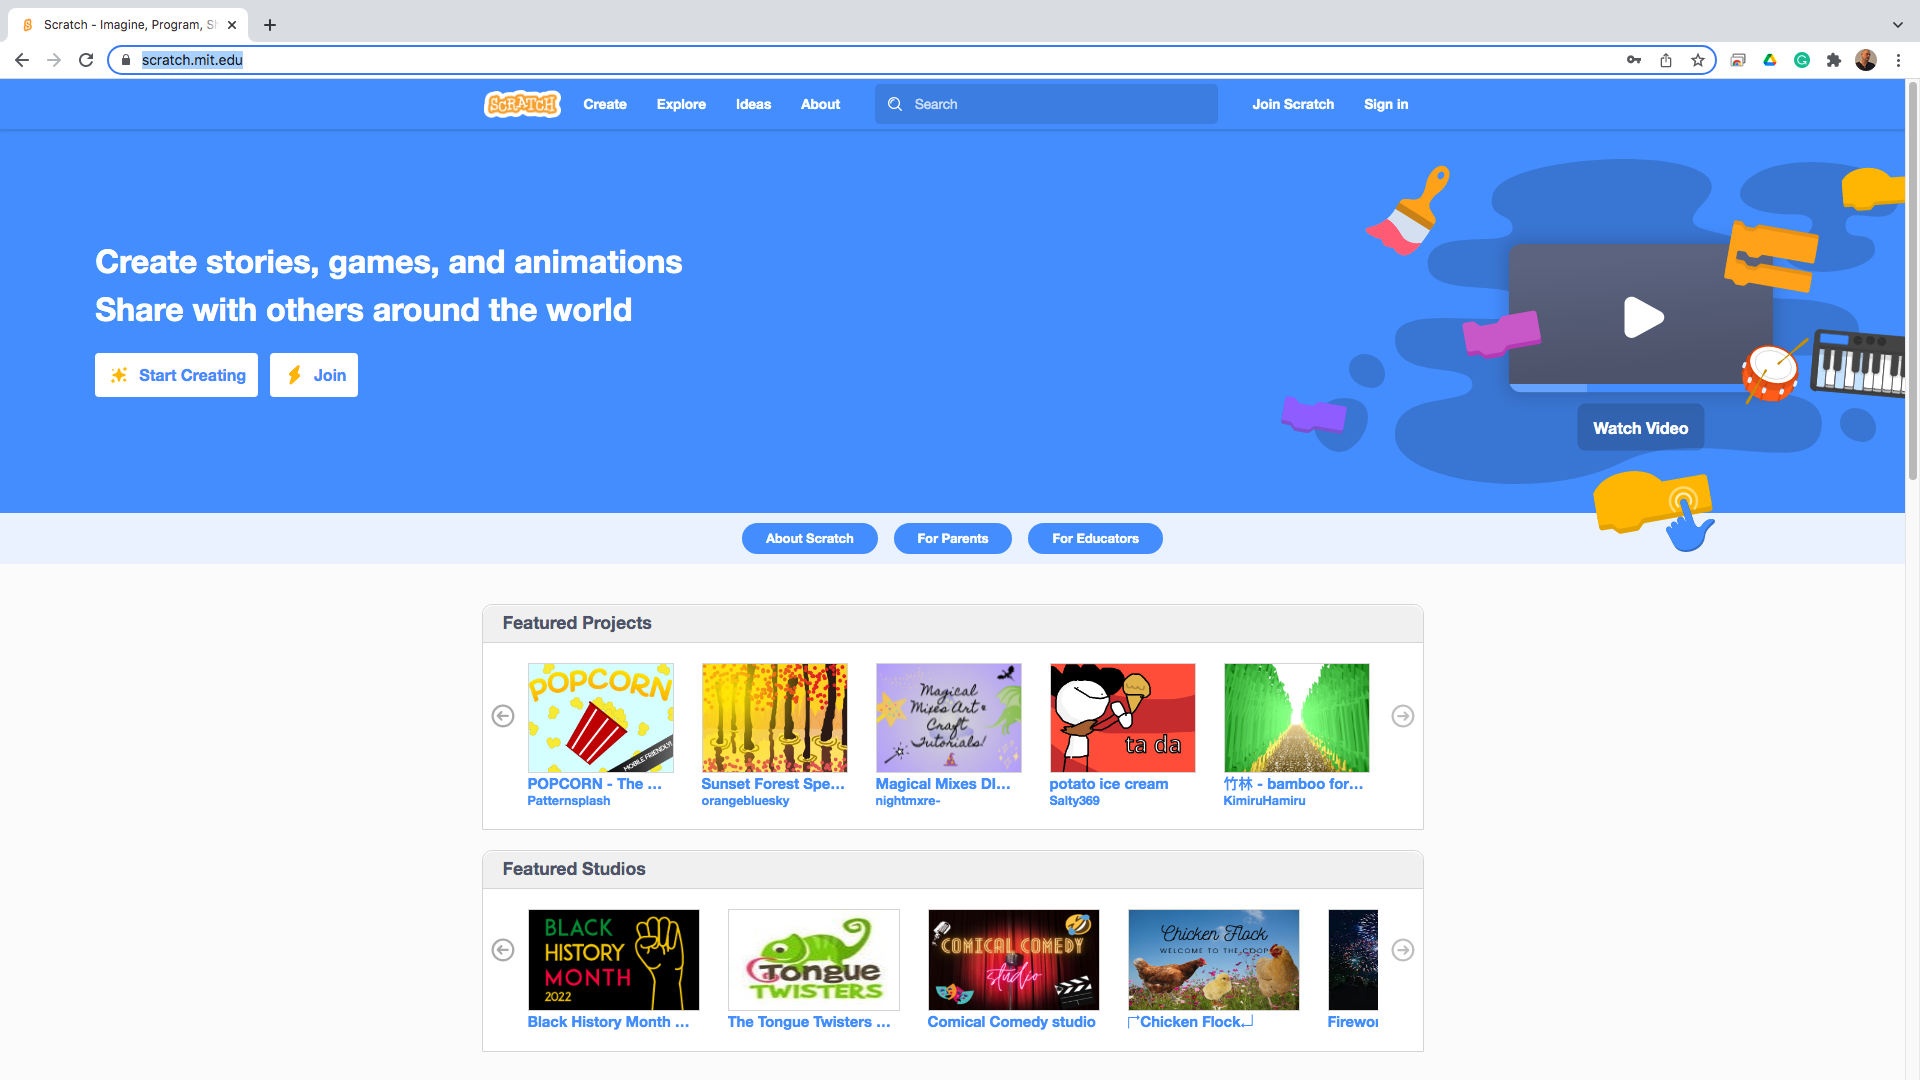
\includegraphics[width=1.0\linewidth,height=0.5\linewidth]{fig010001.png}
  \caption{Начална уеб страница на Sratch}
\label{fig010001}
\end{figure}

Програмната среда на Sratch е организирана на принципа на облачните услуги. Поради тази причина, всеки желаещ да използва услугата трябва да си направи регистрация (Фиг. \ref{fig010002}). Регистрацията се състои от потребителско име и парола.

\begin{figure}[H]
  \centering
  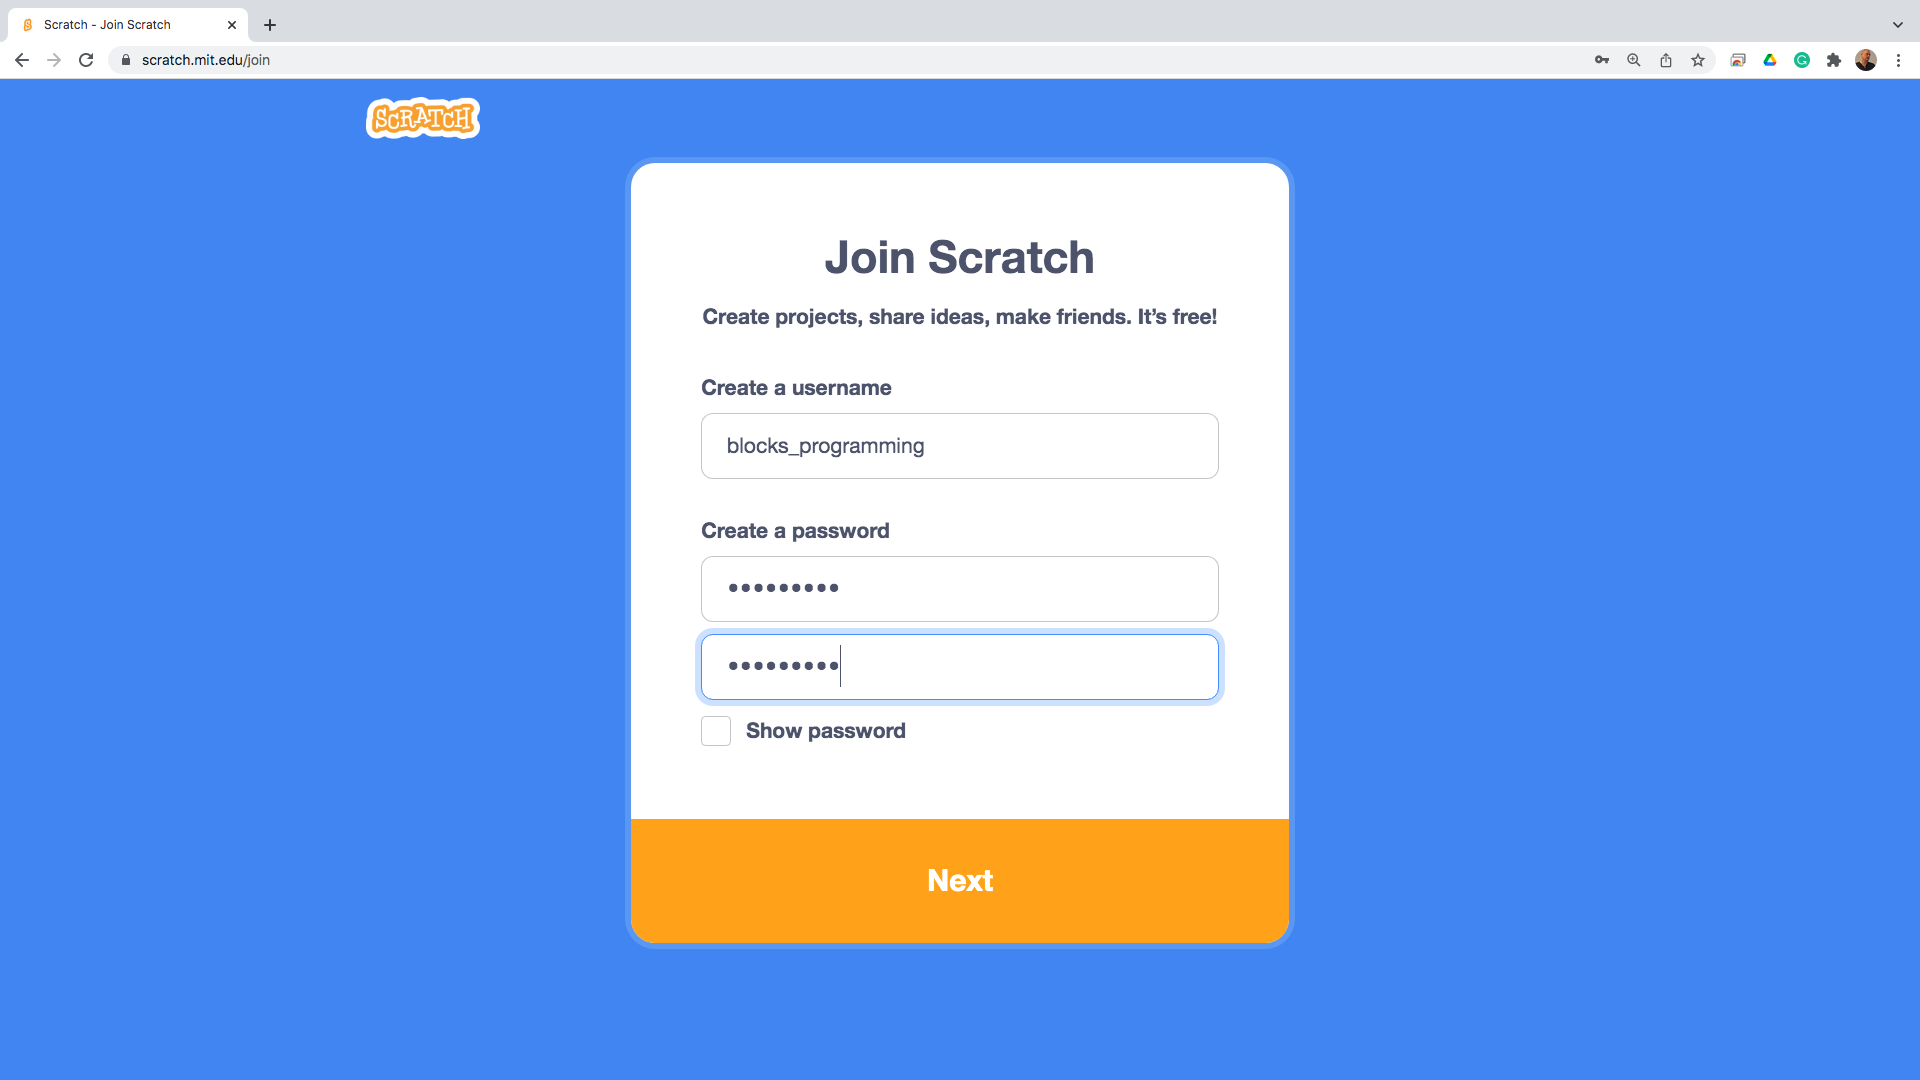
\includegraphics[width=1.0\linewidth,height=0.5\linewidth]{fig010002.png}
  \caption{Регистрация на потребител в Sratch}
\label{fig010002}
\end{figure}

След избора на потребителско име и парола следва определяне на географския регион в който се намира потребителят (Фиг. \ref{fig010003}).

\begin{figure}[H]
  \centering
  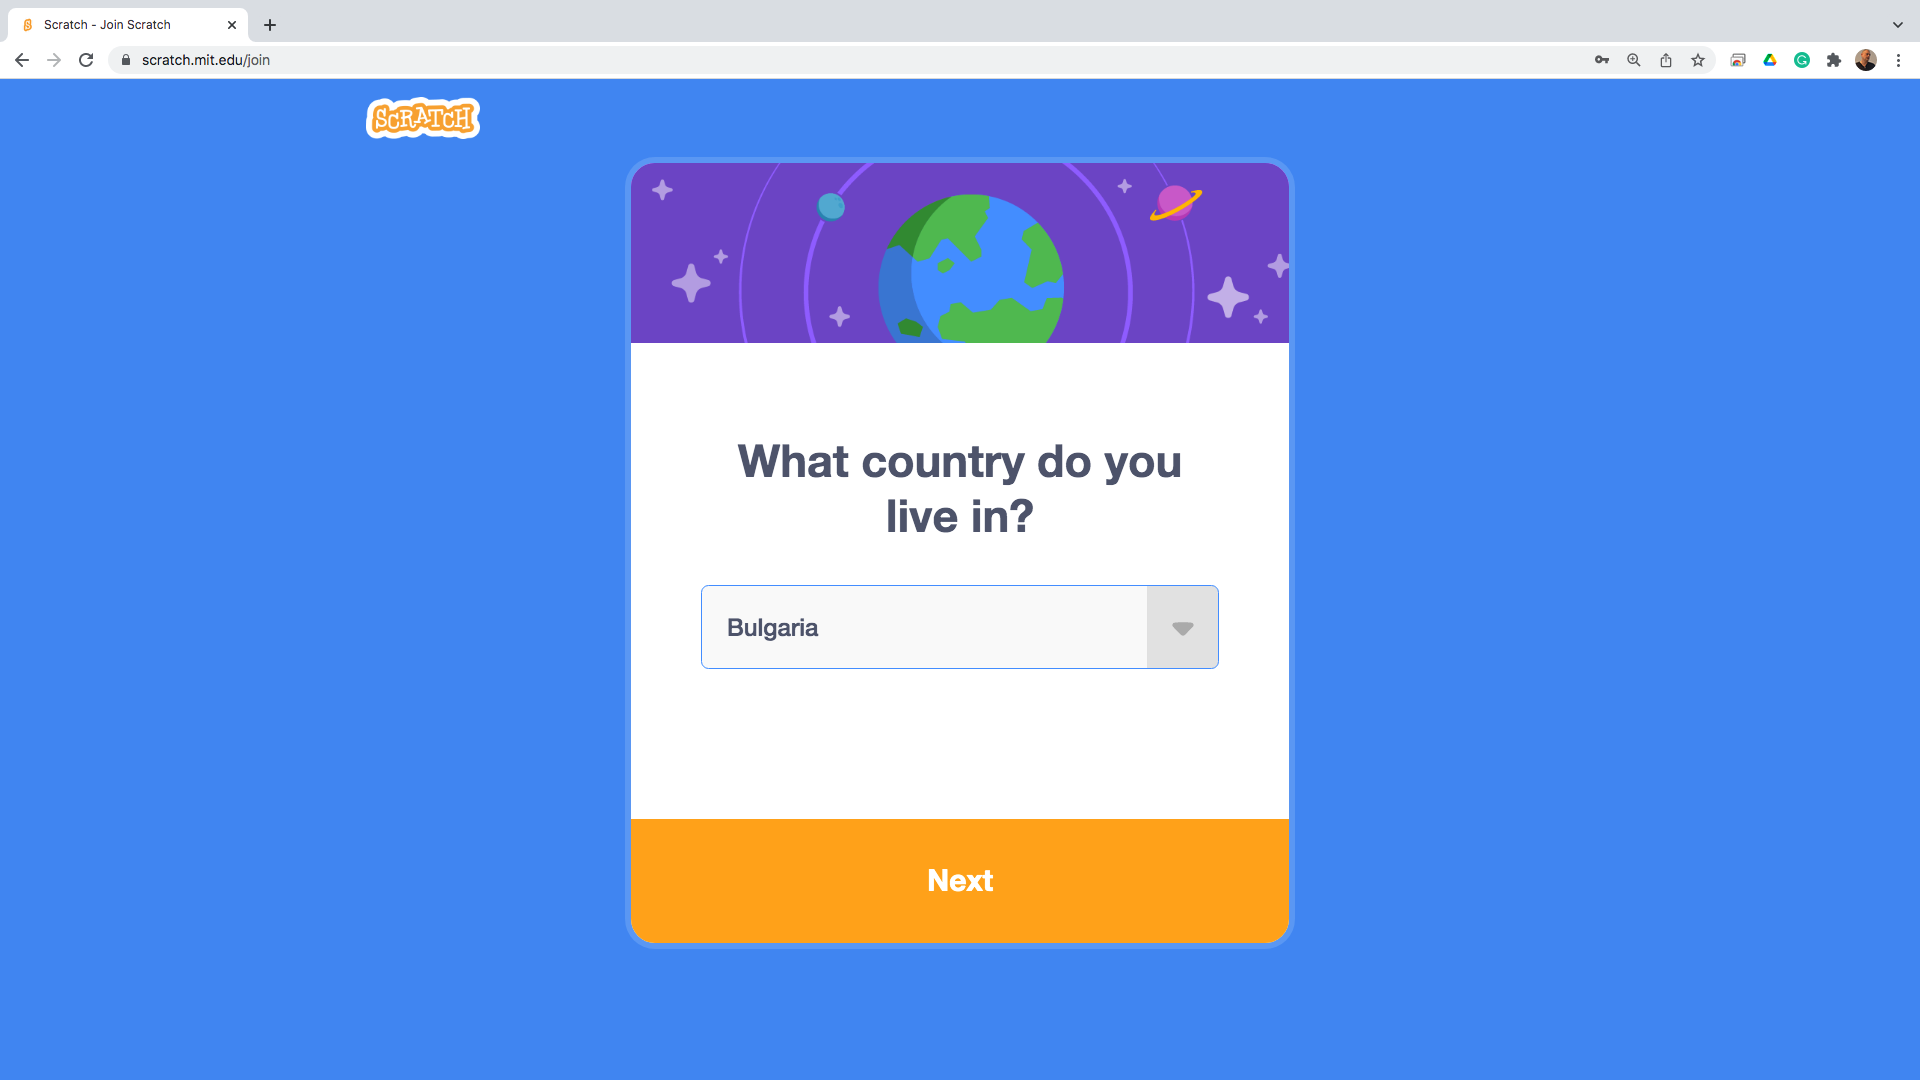
\includegraphics[width=1.0\linewidth,height=0.5\linewidth]{fig010003.png}
  \caption{Географско местоположение}
\label{fig010003}
\end{figure}

Платформата е насочена предимно към деца, изразяващи интерес към програмирането, но също така към родители и учители. Поради тази причина, системата събира информация за възрастта на потребителя (Фиг. \ref{fig010004}).

\begin{figure}[H]
  \centering
  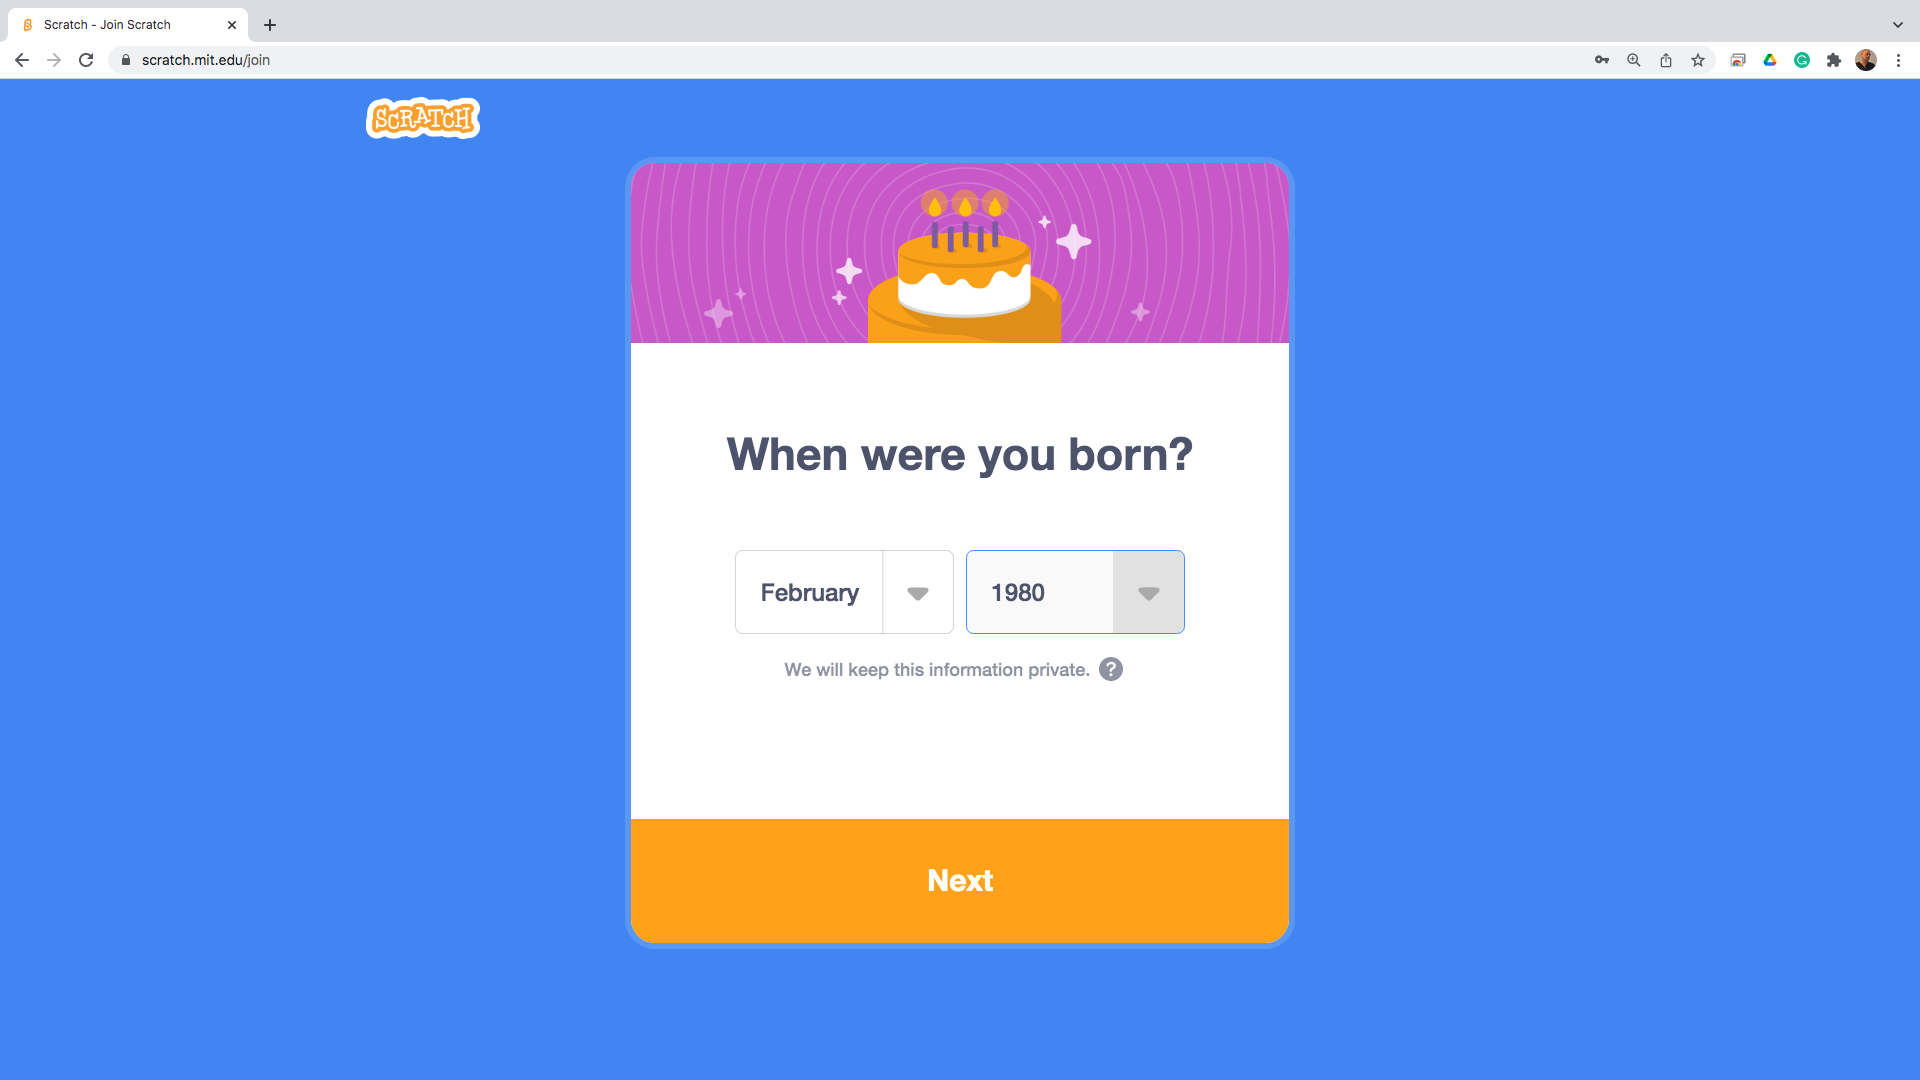
\includegraphics[width=1.0\linewidth,height=0.5\linewidth]{fig010004.png}
  \caption{Възраст на потребителя}
\label{fig010004}
\end{figure}

Освен класификация по възраст, системата събира информация и за класификация по полова принадлежност. Тази информация е незадължителна, основно за да не бъде дискриминираща (Фиг. \ref{fig010005}).

\begin{figure}[H]
  \centering
  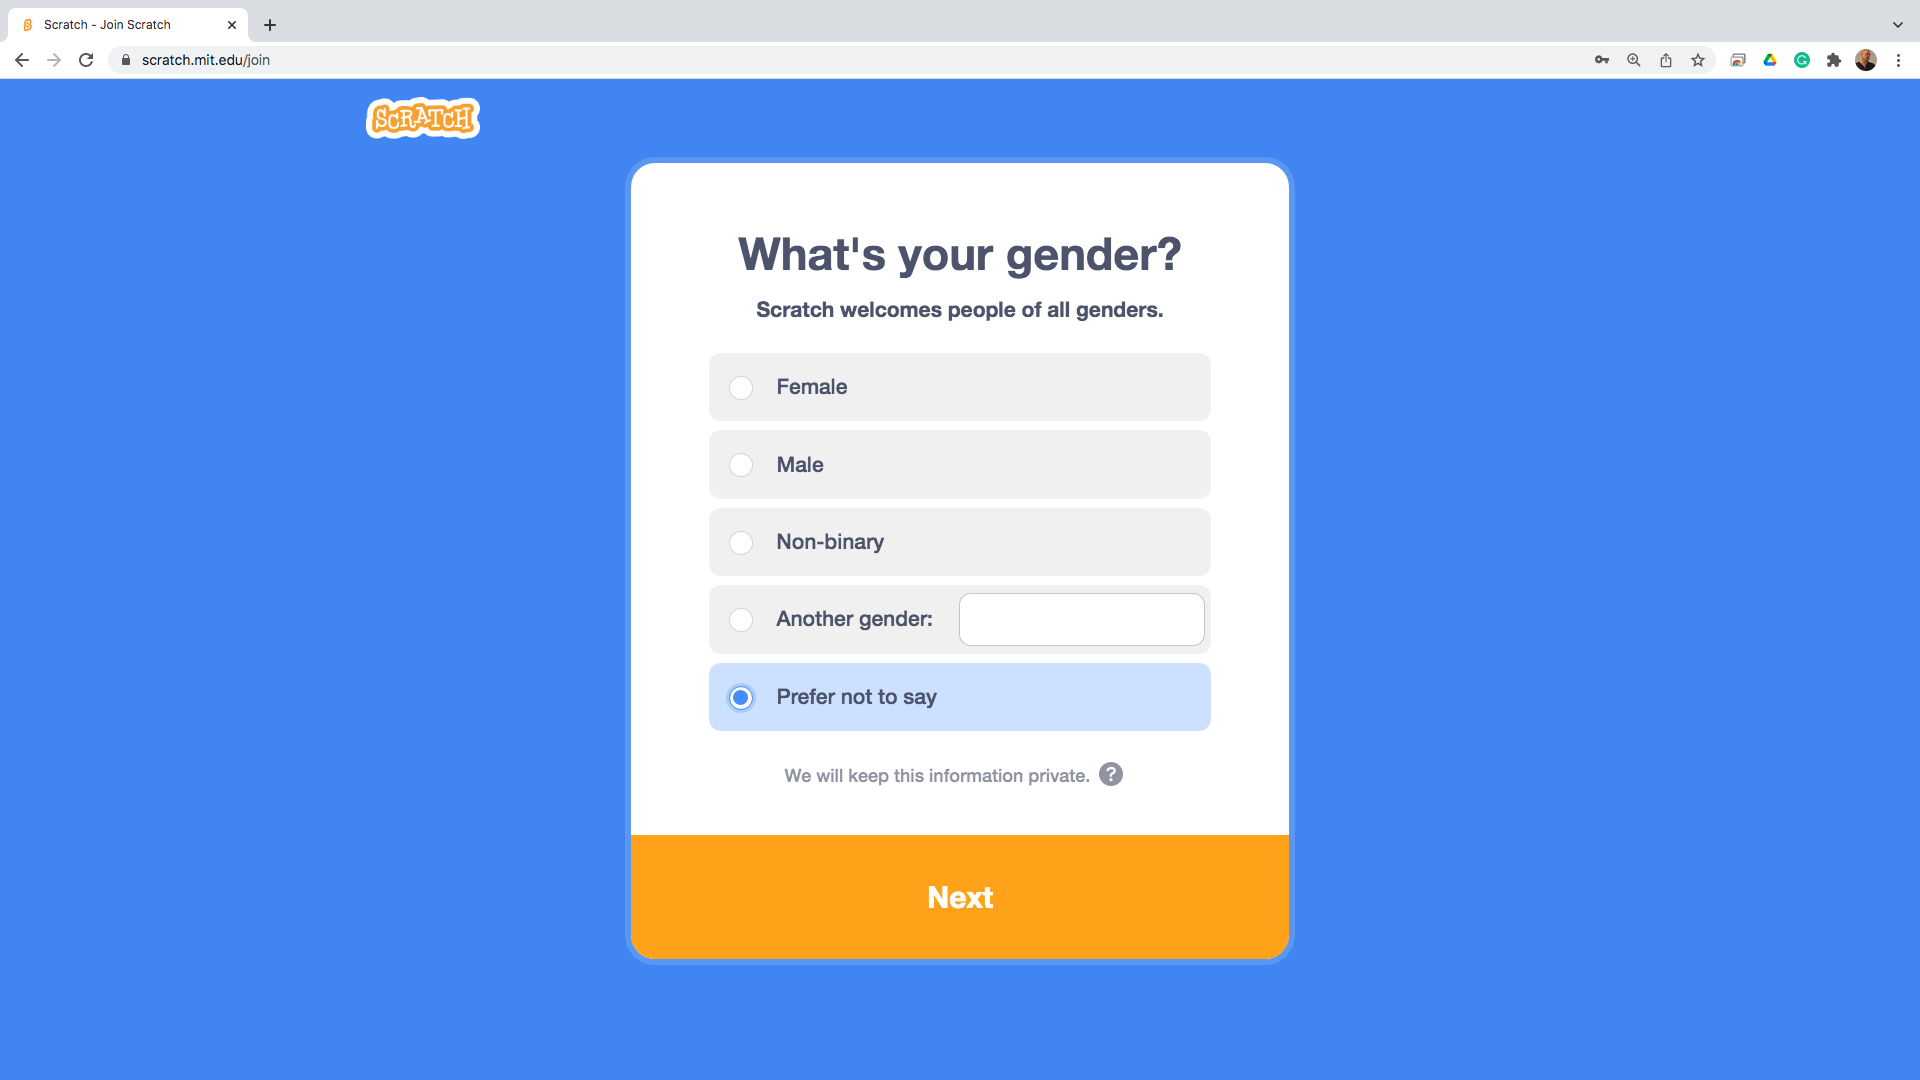
\includegraphics[width=1.0\linewidth,height=0.5\linewidth]{fig010005.png}
  \caption{Пол на потребителя}
\label{fig010005}
\end{figure}

Потребителският профил, освен с потребителско име и парола, трябва да бъде аоцииран и с адрес на електронна пощенска кутия (Фиг. \ref{fig010006}).

\begin{figure}[H]
  \centering
  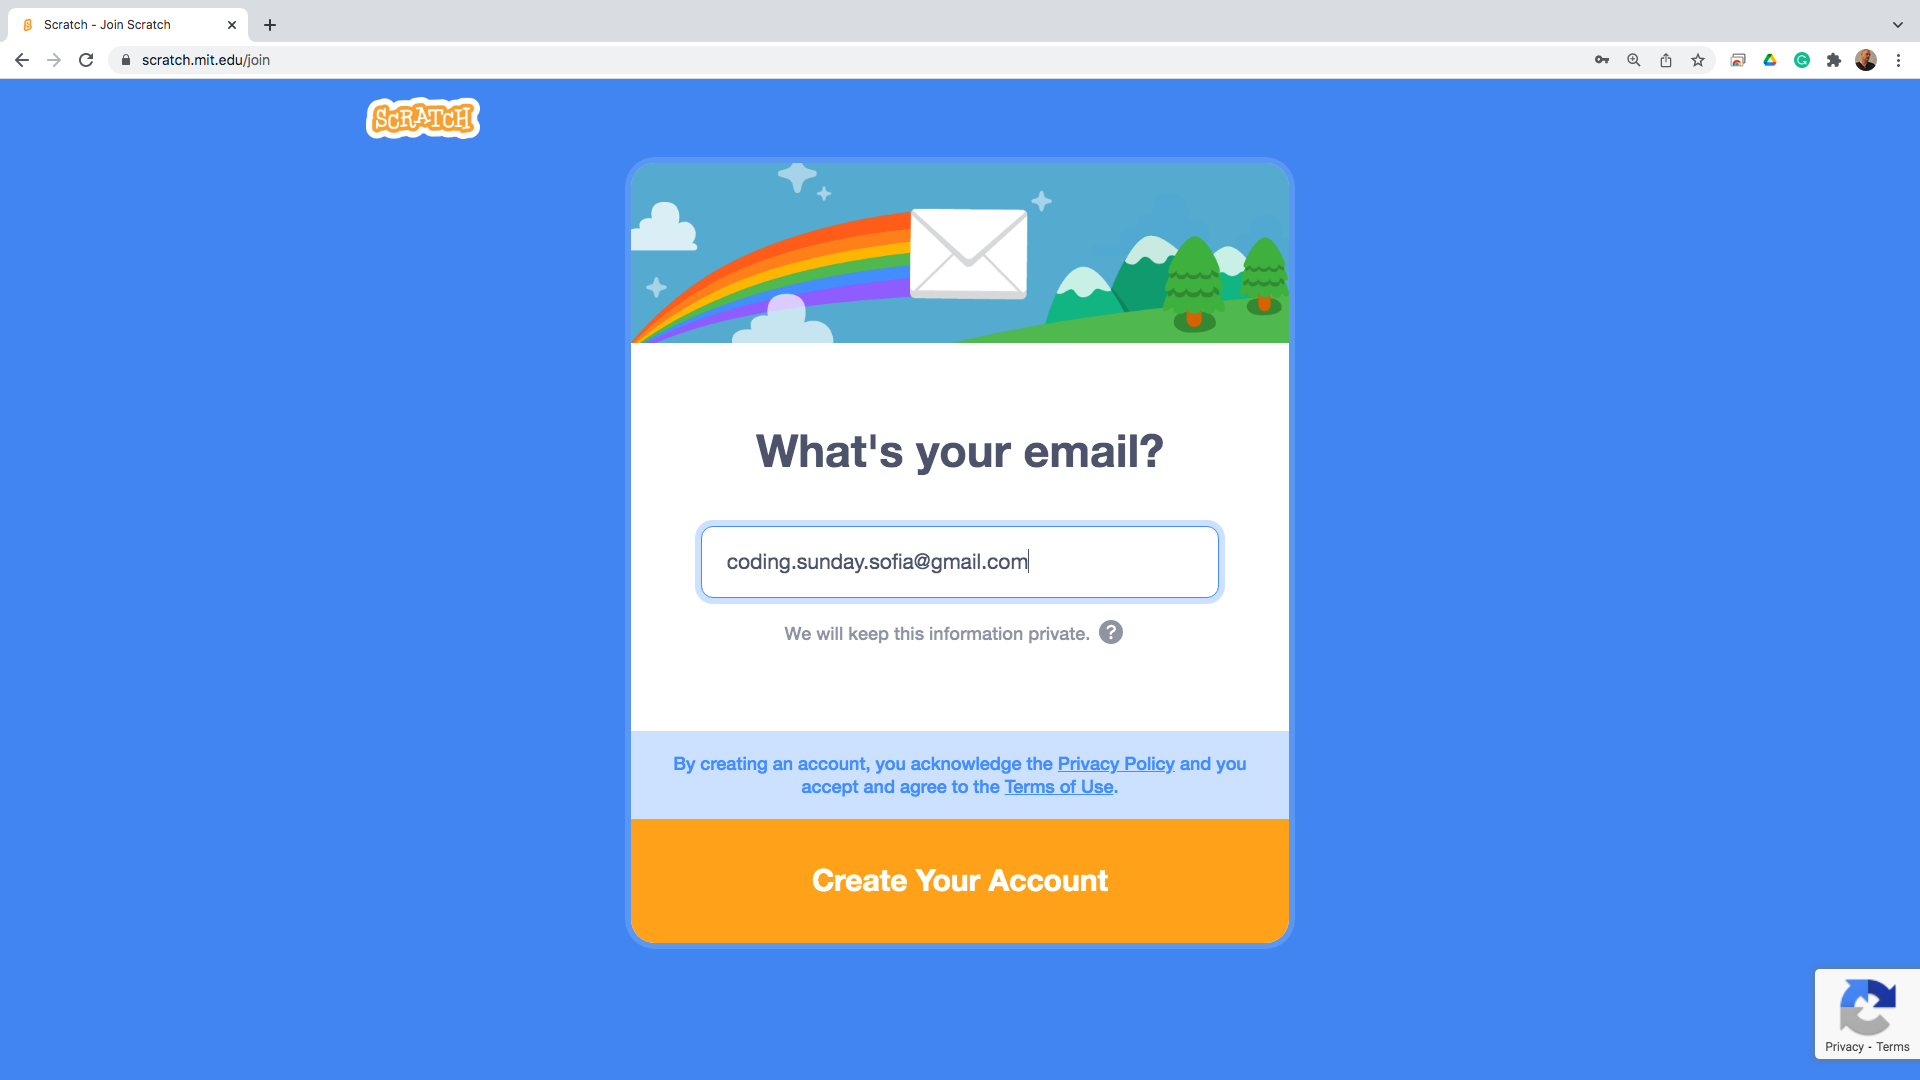
\includegraphics[width=1.0\linewidth,height=0.5\linewidth]{fig010006.png}
  \caption{Адрес на електронна поща на потребителя}
\label{fig010006}
\end{figure}

Процесът по регистрация на потребител в системата е почти завършен (Фиг. \ref{fig010007}). Остава само стъпката за потвърждаване на избрания адрес за електронна поща.

\begin{figure}[H]
  \centering
  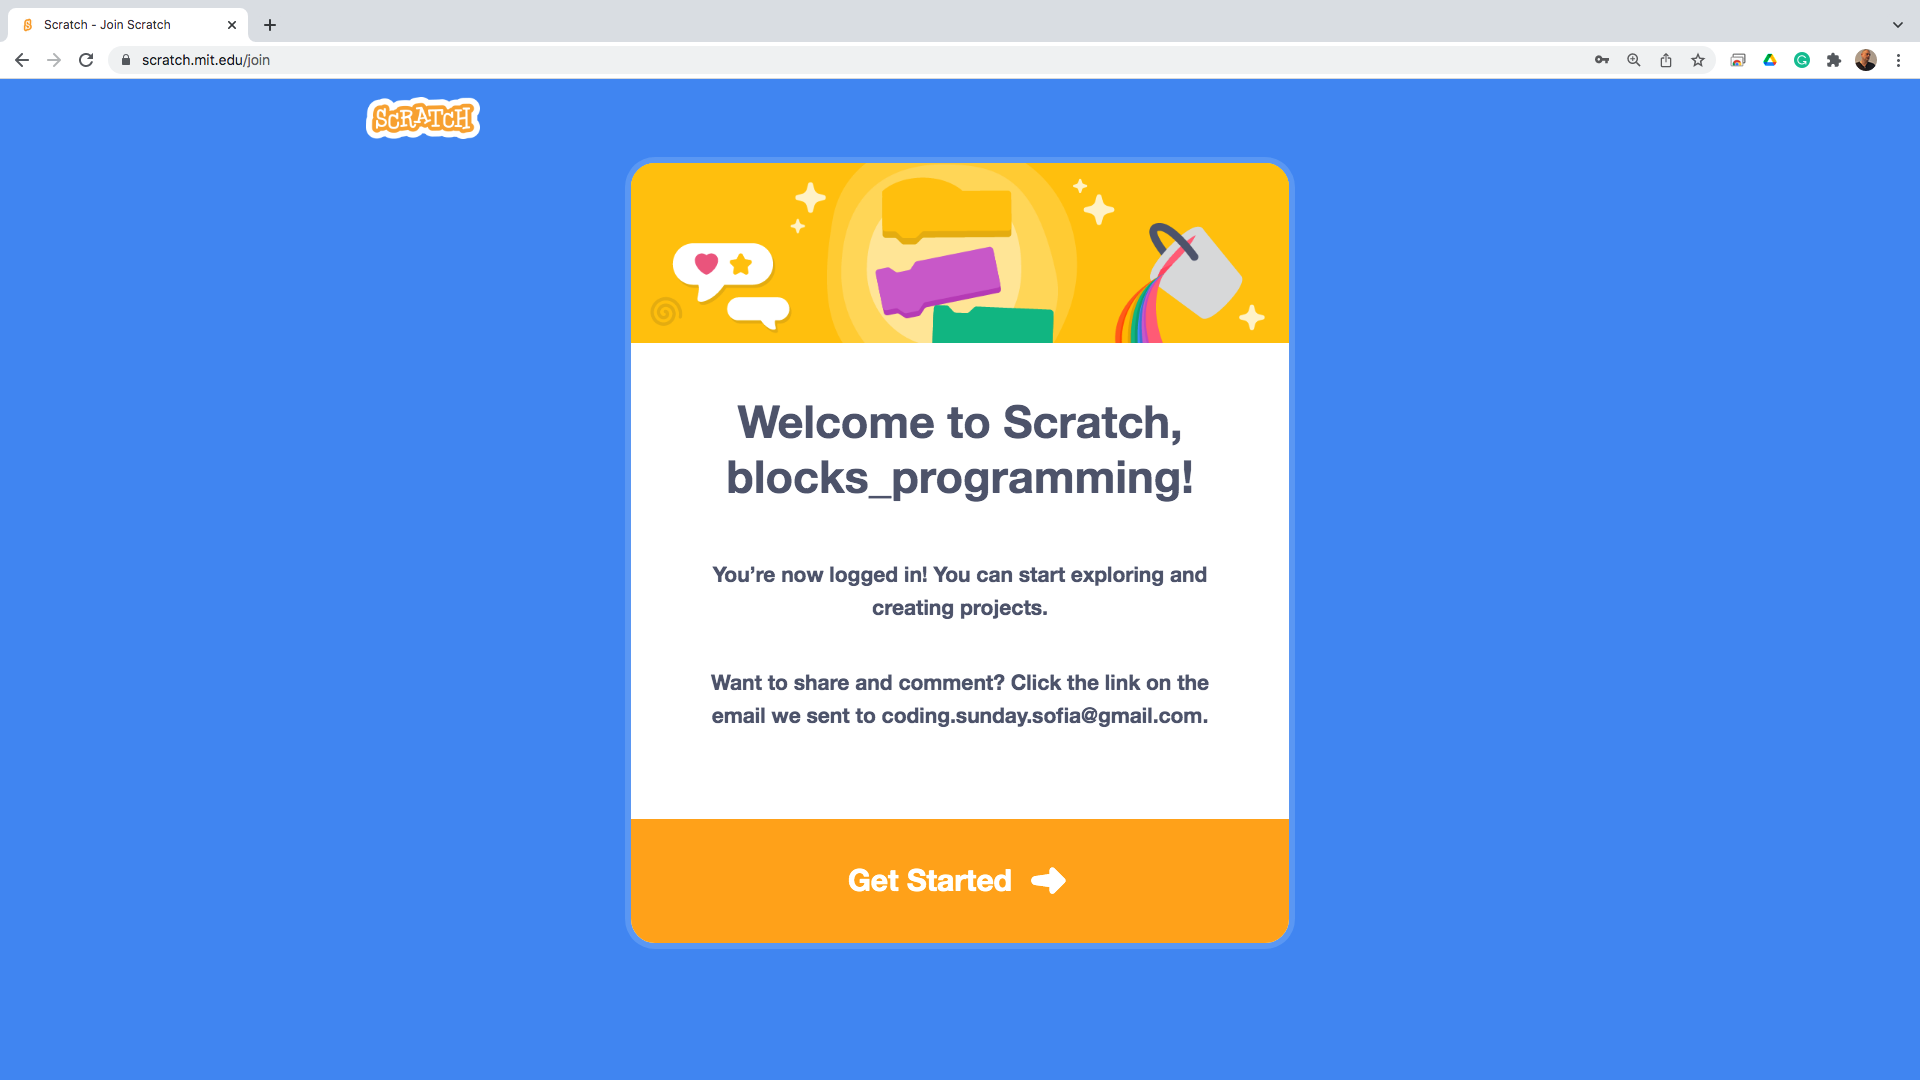
\includegraphics[width=1.0\linewidth,height=0.5\linewidth]{fig010007.png}
  \caption{Приключване на процеса за въвеждане на информация за потребителя}
\label{fig010007}
\end{figure}

Електронното писмо, за потвърждаване на потребителската регистрация, съдържа електронна препратка до уеб сайта на Sratch (Фиг. \ref{fig010008}). Тази препратка трябва да бъде последвана за да се завърши процесът по регистрация на нов потребител. 

\begin{figure}[H]
  \centering
  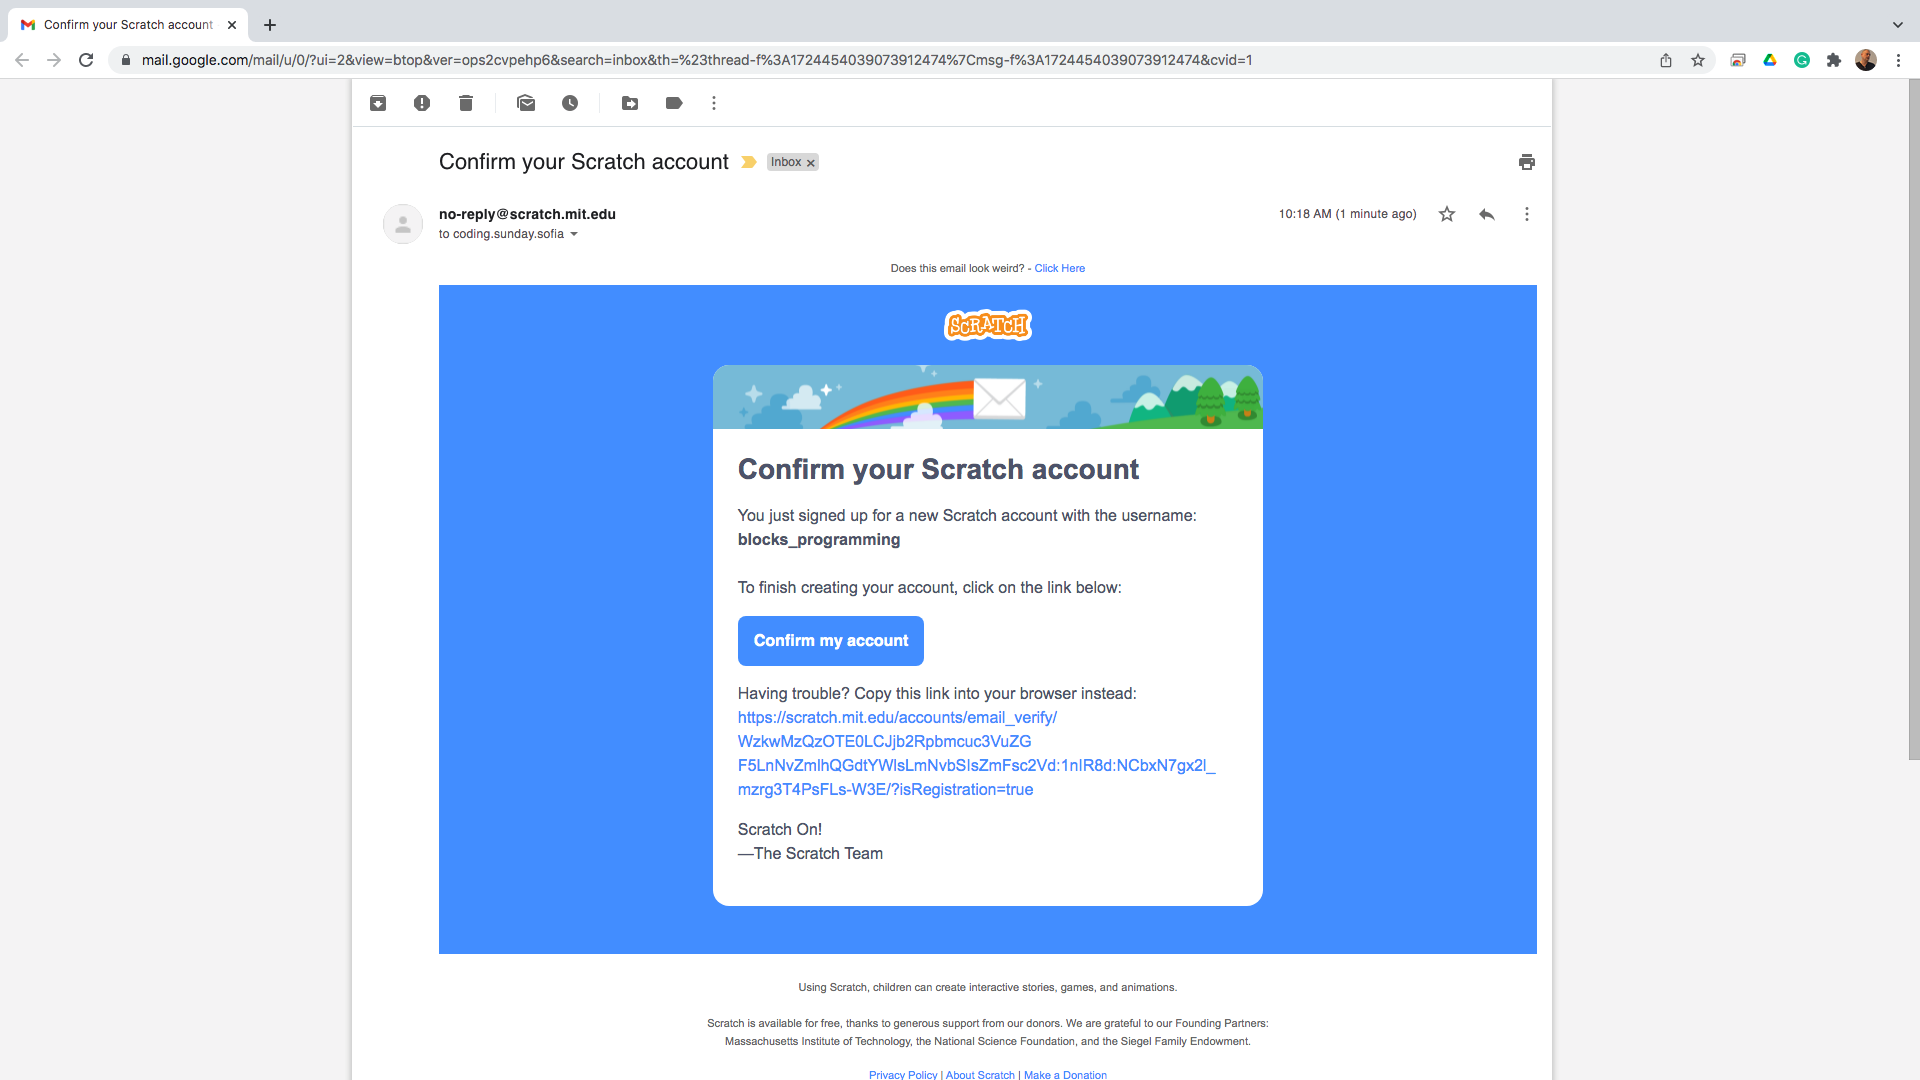
\includegraphics[width=1.0\linewidth,height=0.5\linewidth]{fig010008.png}
  \caption{Електронно съобщение за потвърждаване на електронния адрес}
\label{fig010008}
\end{figure}

Регистрацията на новия потребител приключва със зареждането на начален работен екран (Фиг. \ref{fig010009}). Горе, в дясно се вижда изписано потребителското име, избрано на първата стъпка от процеса по регистрацията.

\begin{figure}[H]
  \centering
  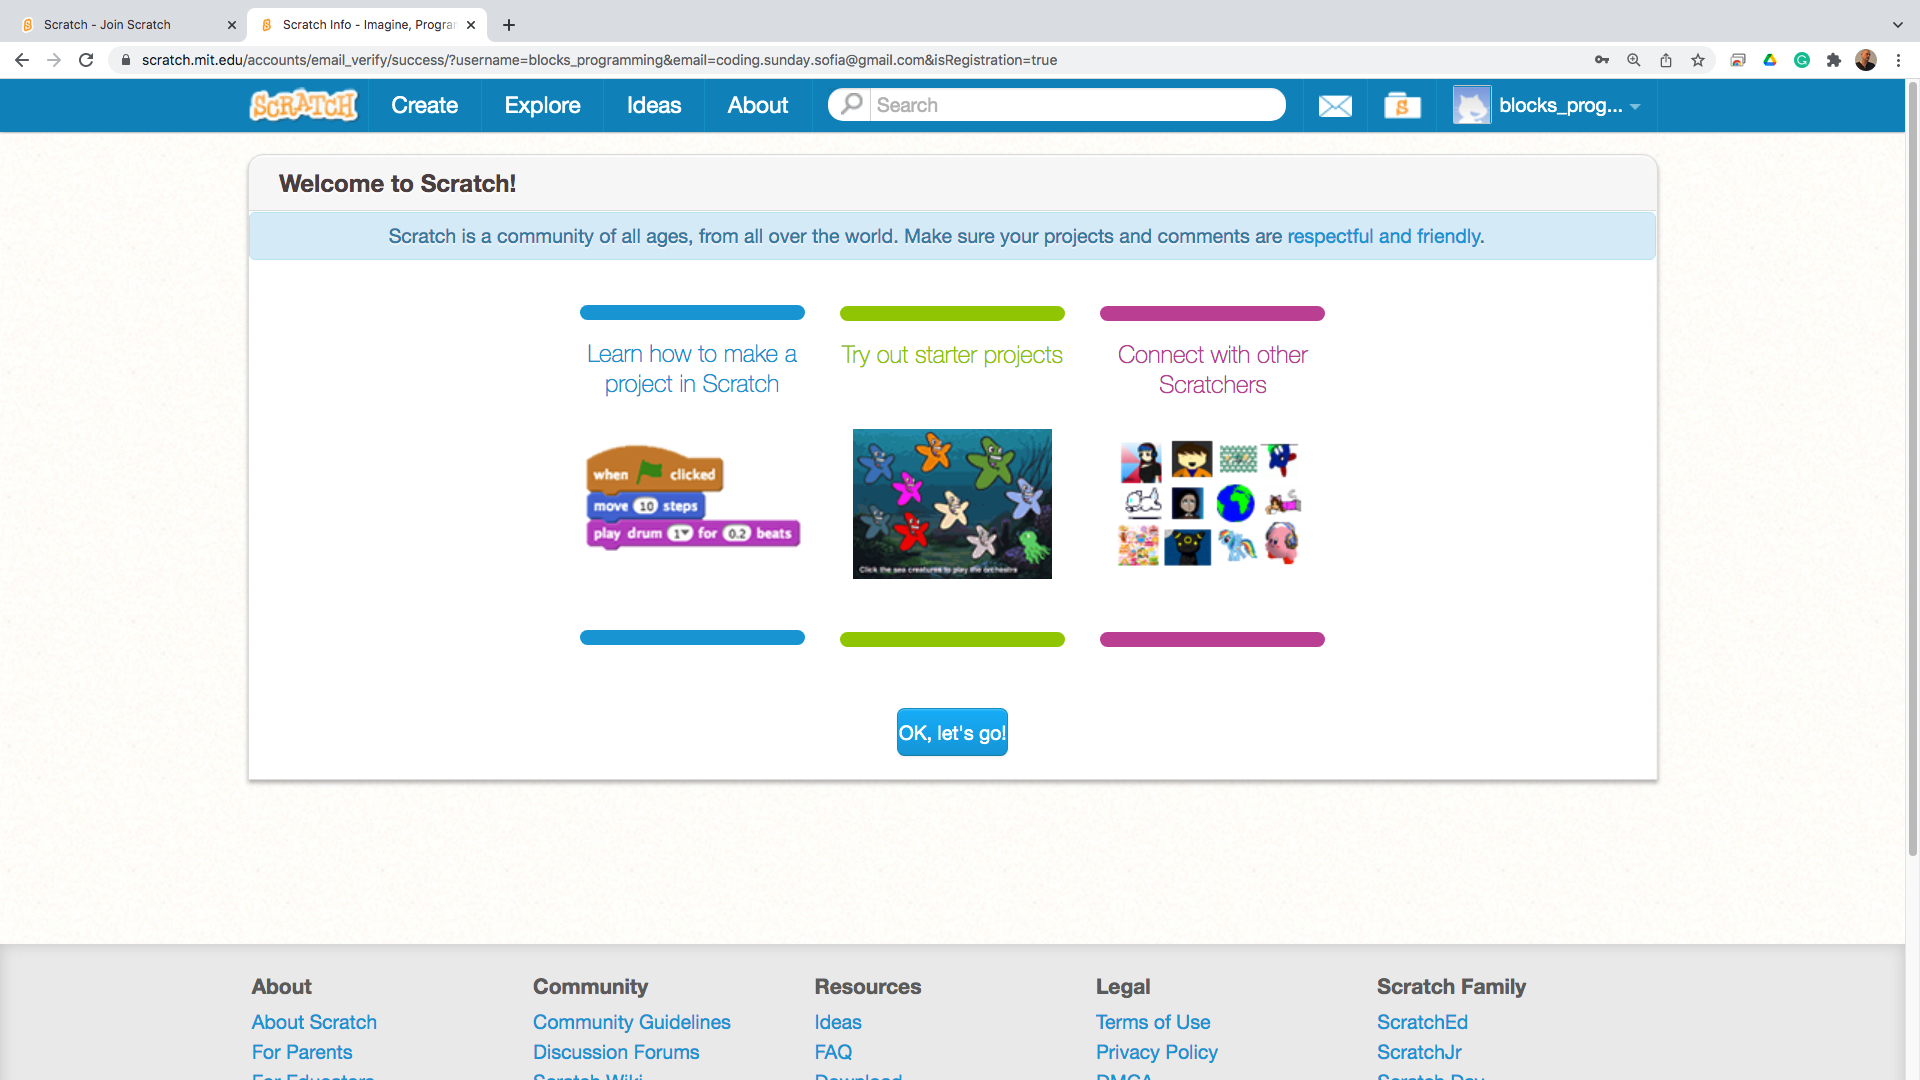
\includegraphics[width=1.0\linewidth,height=0.5\linewidth]{fig010009.png}
  \caption{Начален работен екран}
\label{fig010009}
\end{figure}

Успешната регистрация може да се потвърди и чрез създаването на много малък проект, който да демонстрира функционирането на развойната среда. За тази цел се избира опцията „Create“ от менюто (Фиг. \ref{fig010010}).

\begin{figure}[H]
  \centering
  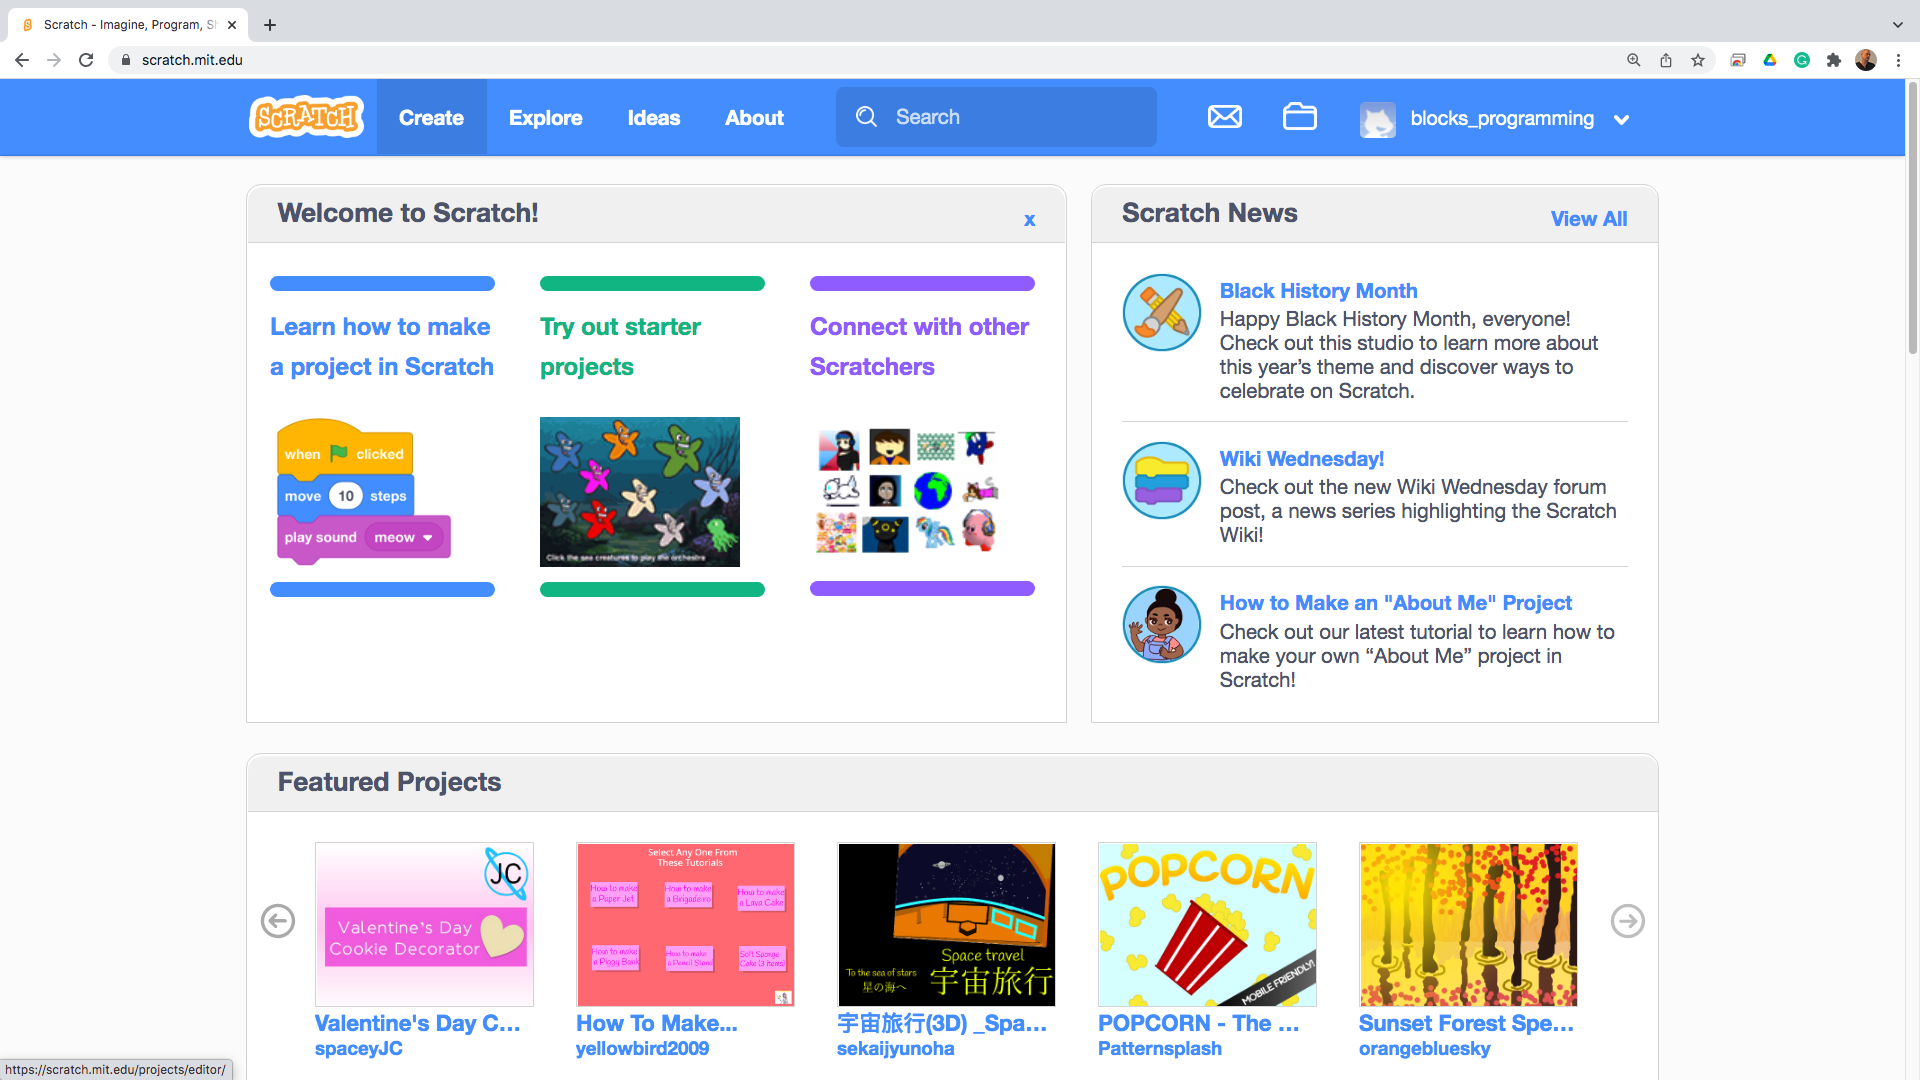
\includegraphics[width=1.0\linewidth,height=0.5\linewidth]{fig010010.png}
  \caption{Избор на опция от менюто за нов проект}
\label{fig010010}
\end{figure}

Създаването на нов проект преминава през серия стъпки, свързани със заделянето на първоначално нужните ресурси (Фиг. \ref{fig010011}).

\begin{figure}[H]
  \centering
  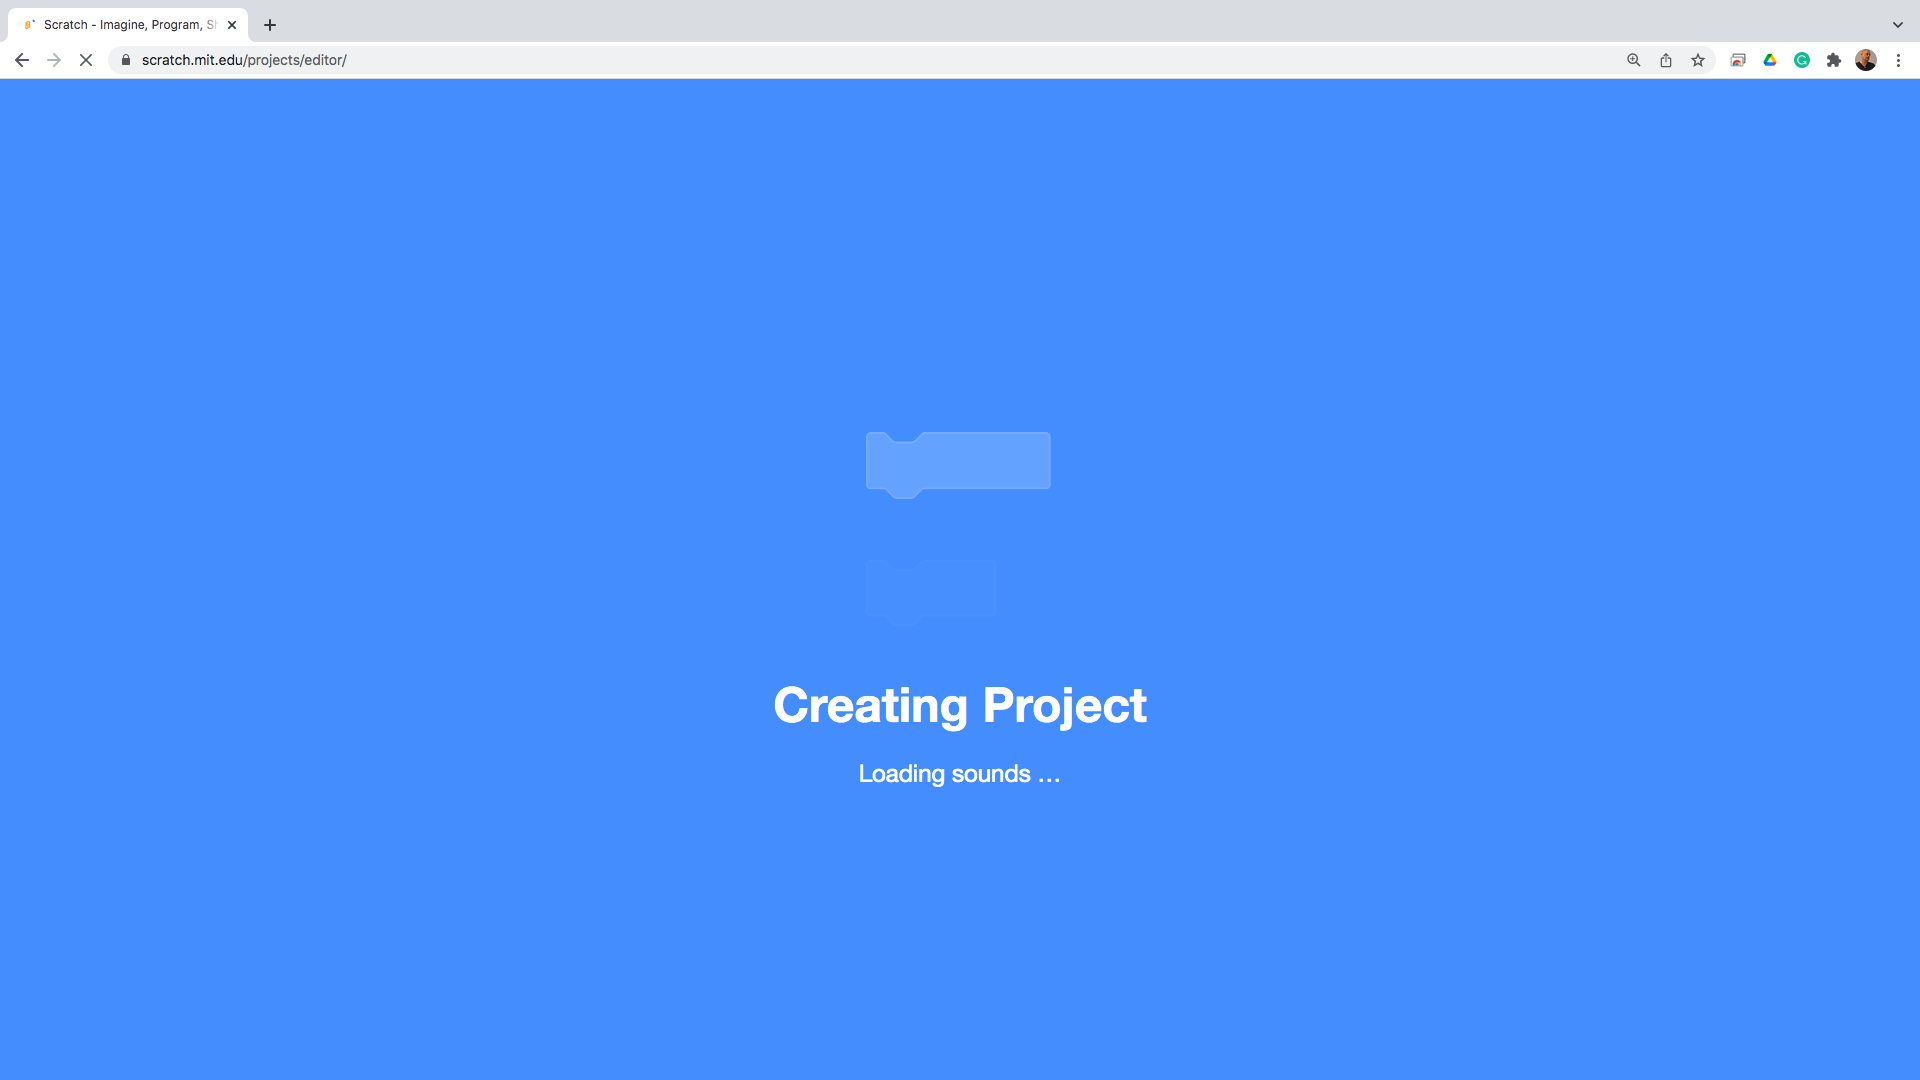
\includegraphics[width=1.0\linewidth,height=0.5\linewidth]{fig010011.png}
  \caption{Зареждане на ресурсите}
\label{fig010011}
\end{figure}

След зареждането на новия проект се визуализира работното пространство (Фиг. \ref{fig010012}). Най- в ляво е списъкът с възможни програмни инструкции, под формата на парченца от пъзел. В централната част е работното пространство, където инструкциите се подреждат. А най- в дясно е активната сцена, където се визуализират действията, заложени в серията от инструкции. 

\begin{figure}[H]
  \centering
  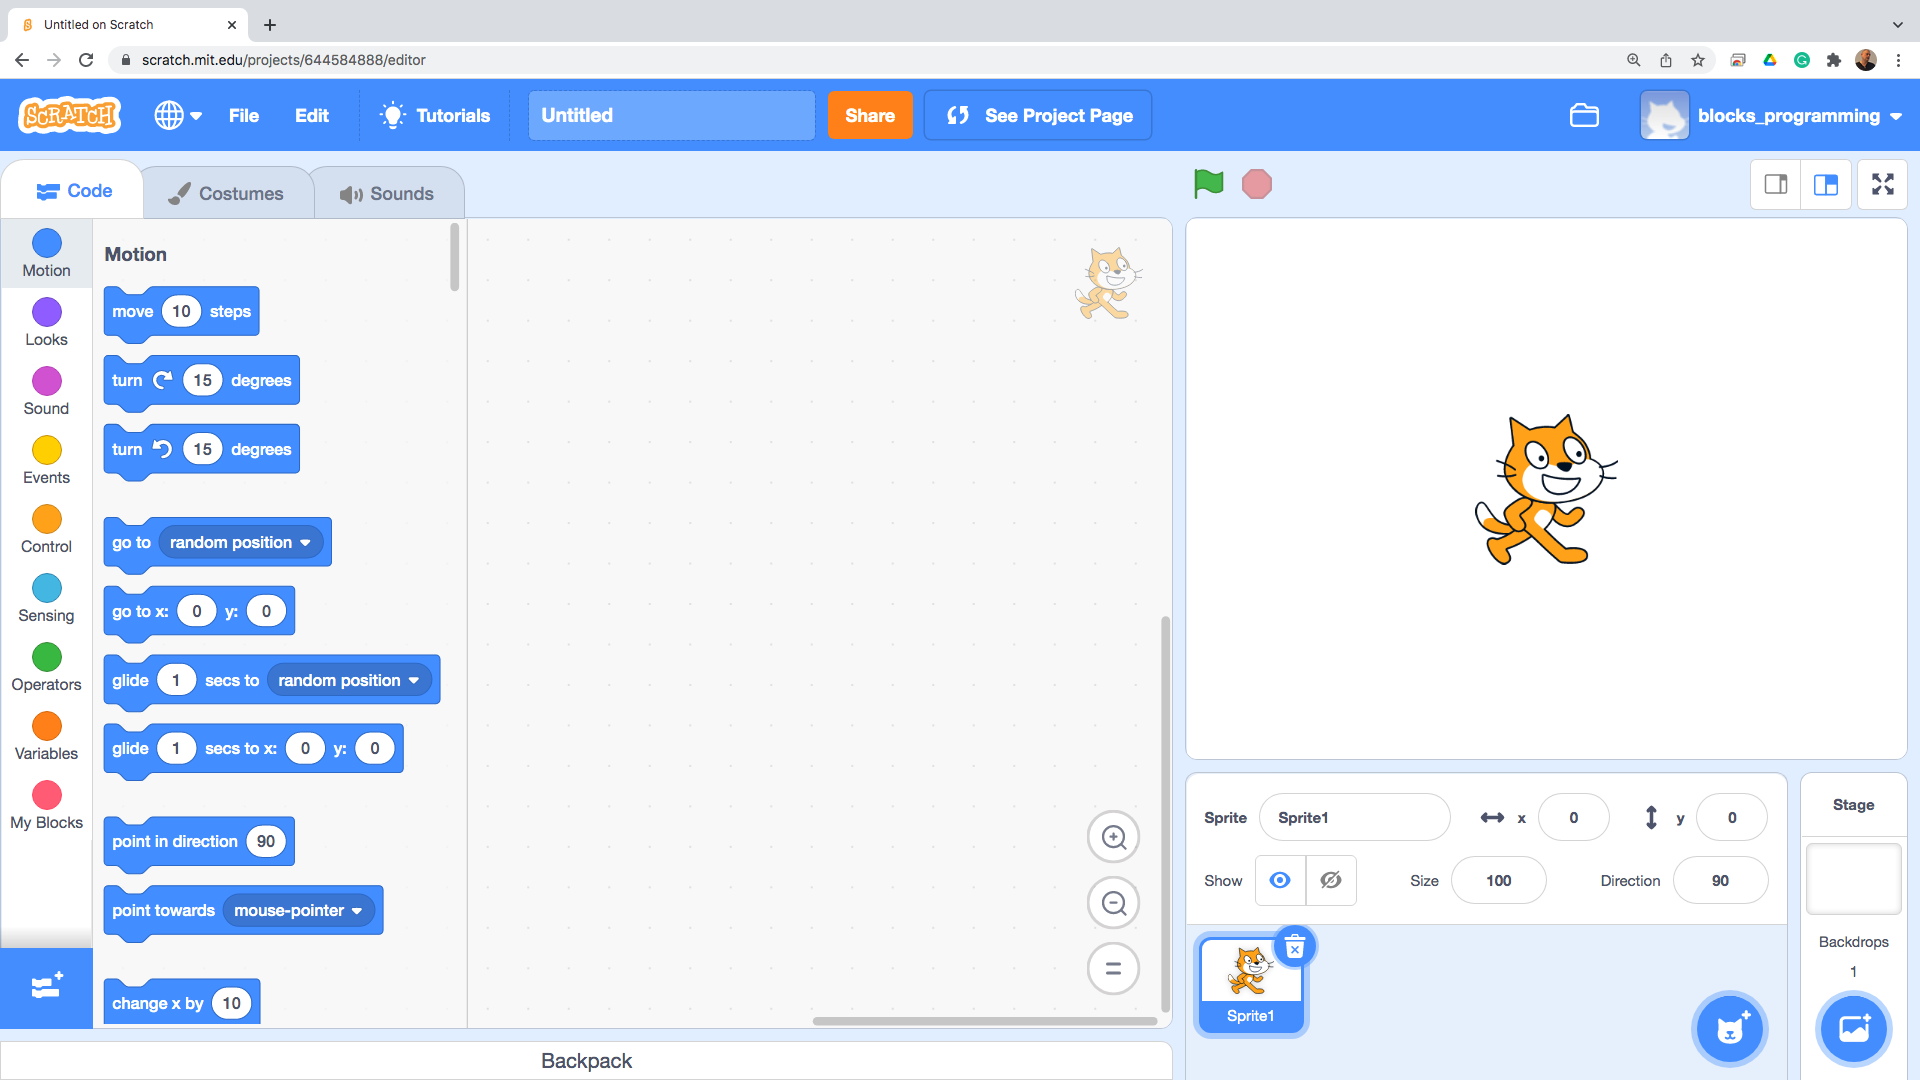
\includegraphics[width=1.0\linewidth,height=0.5\linewidth]{fig010012.png}
  \caption{Организация на работното пространство}
\label{fig010012}
\end{figure}

Всяка компютърна програма има своя начална точка и своя крайна точка. В Scratch, за началото на програмата има специално отделен блок (програмна инструкция), която е показна на Фиг. \ref{fig010013}. Изпълнението на програмите, написани в Scratch, започва с натискането на зеления флаг. Точно поради тази причина, блокчето за старт на програмата е свързано със събитието за натискане на зеления флаг. 

\begin{figure}[H]
  \centering
  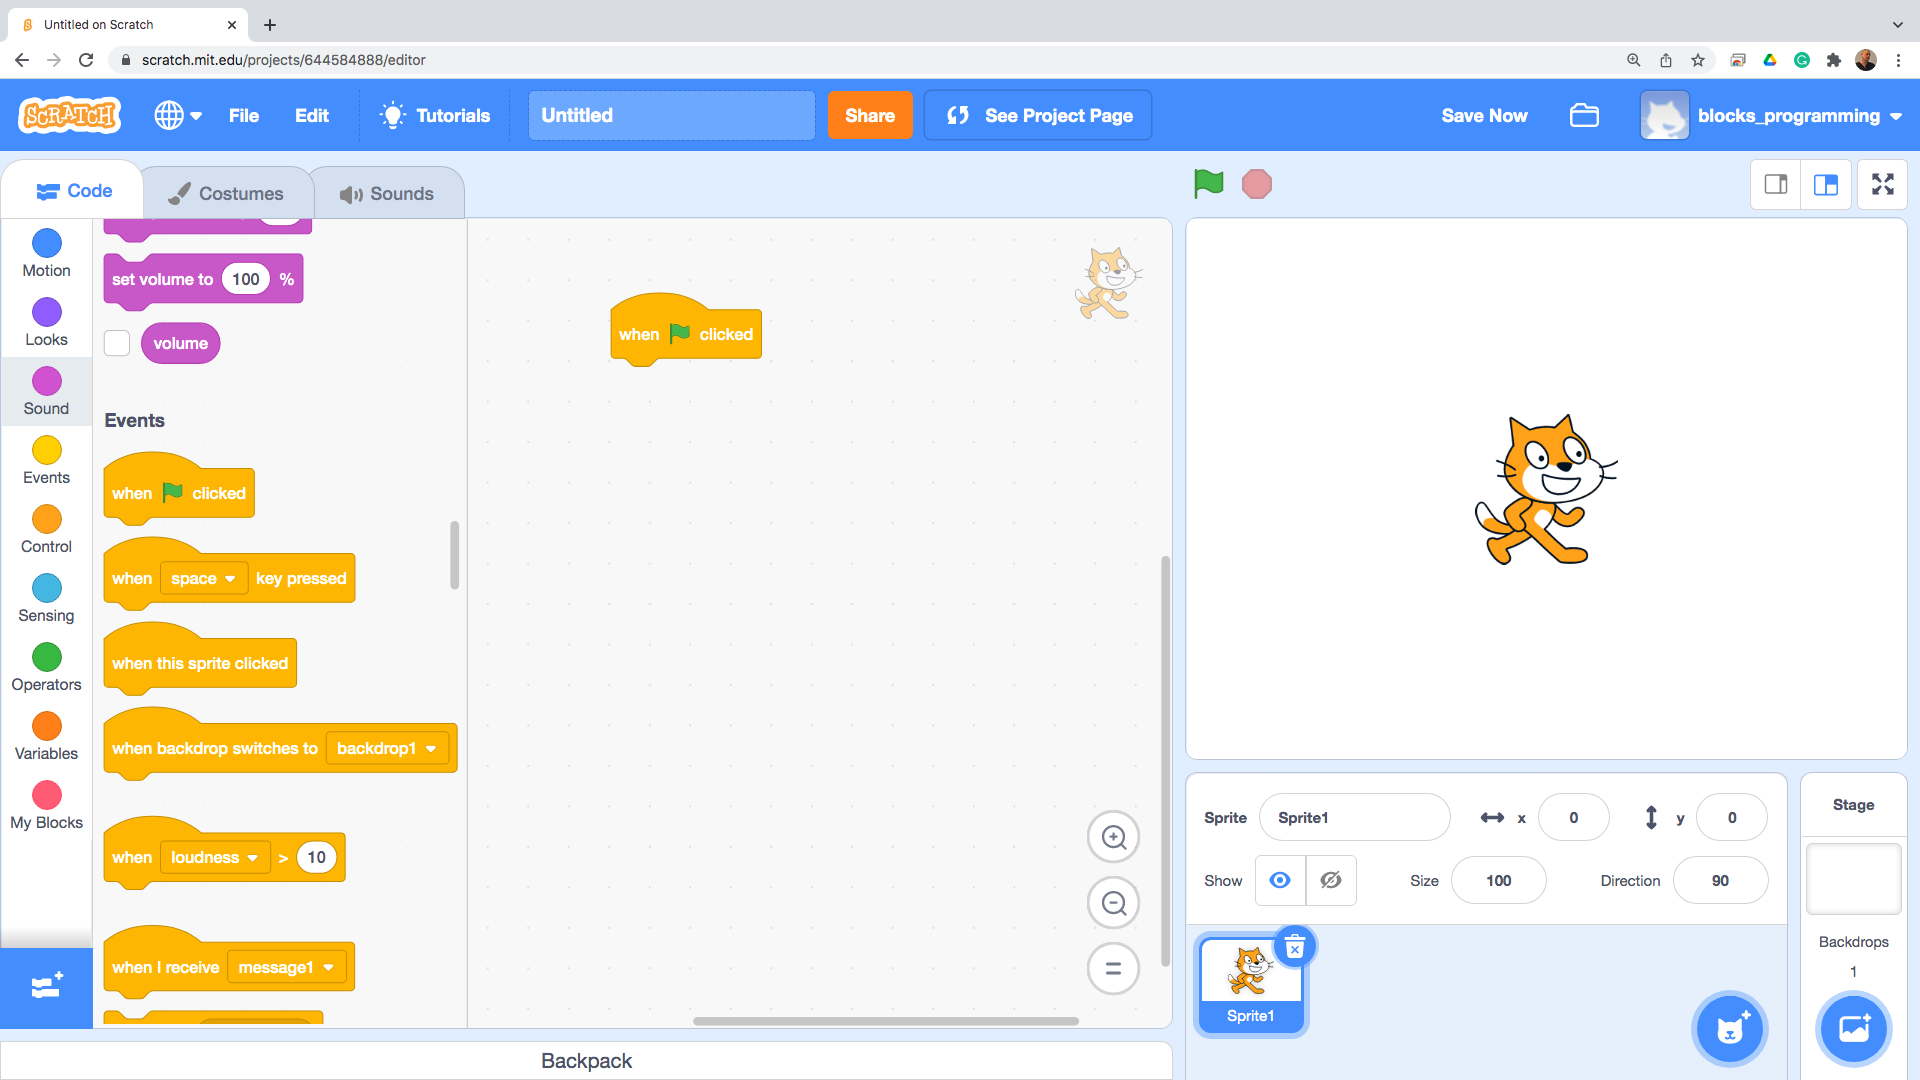
\includegraphics[width=1.0\linewidth,height=0.5\linewidth]{fig010013.png}
  \caption{Начало на програмата}
\label{fig010013}
\end{figure}

Една от най-интуитивните и същевременно лесно разбираеми инструкции е преместване с определен брой стъпки (Фиг. \ref{fig010014}). Главен актьор в началната сцена на Scratch е оранжевият котарак. Ако сцената не бъде променяна, то инструкциите за извършване на различни действия се насочват точно към този котарак. 

\begin{figure}[H]
  \centering
  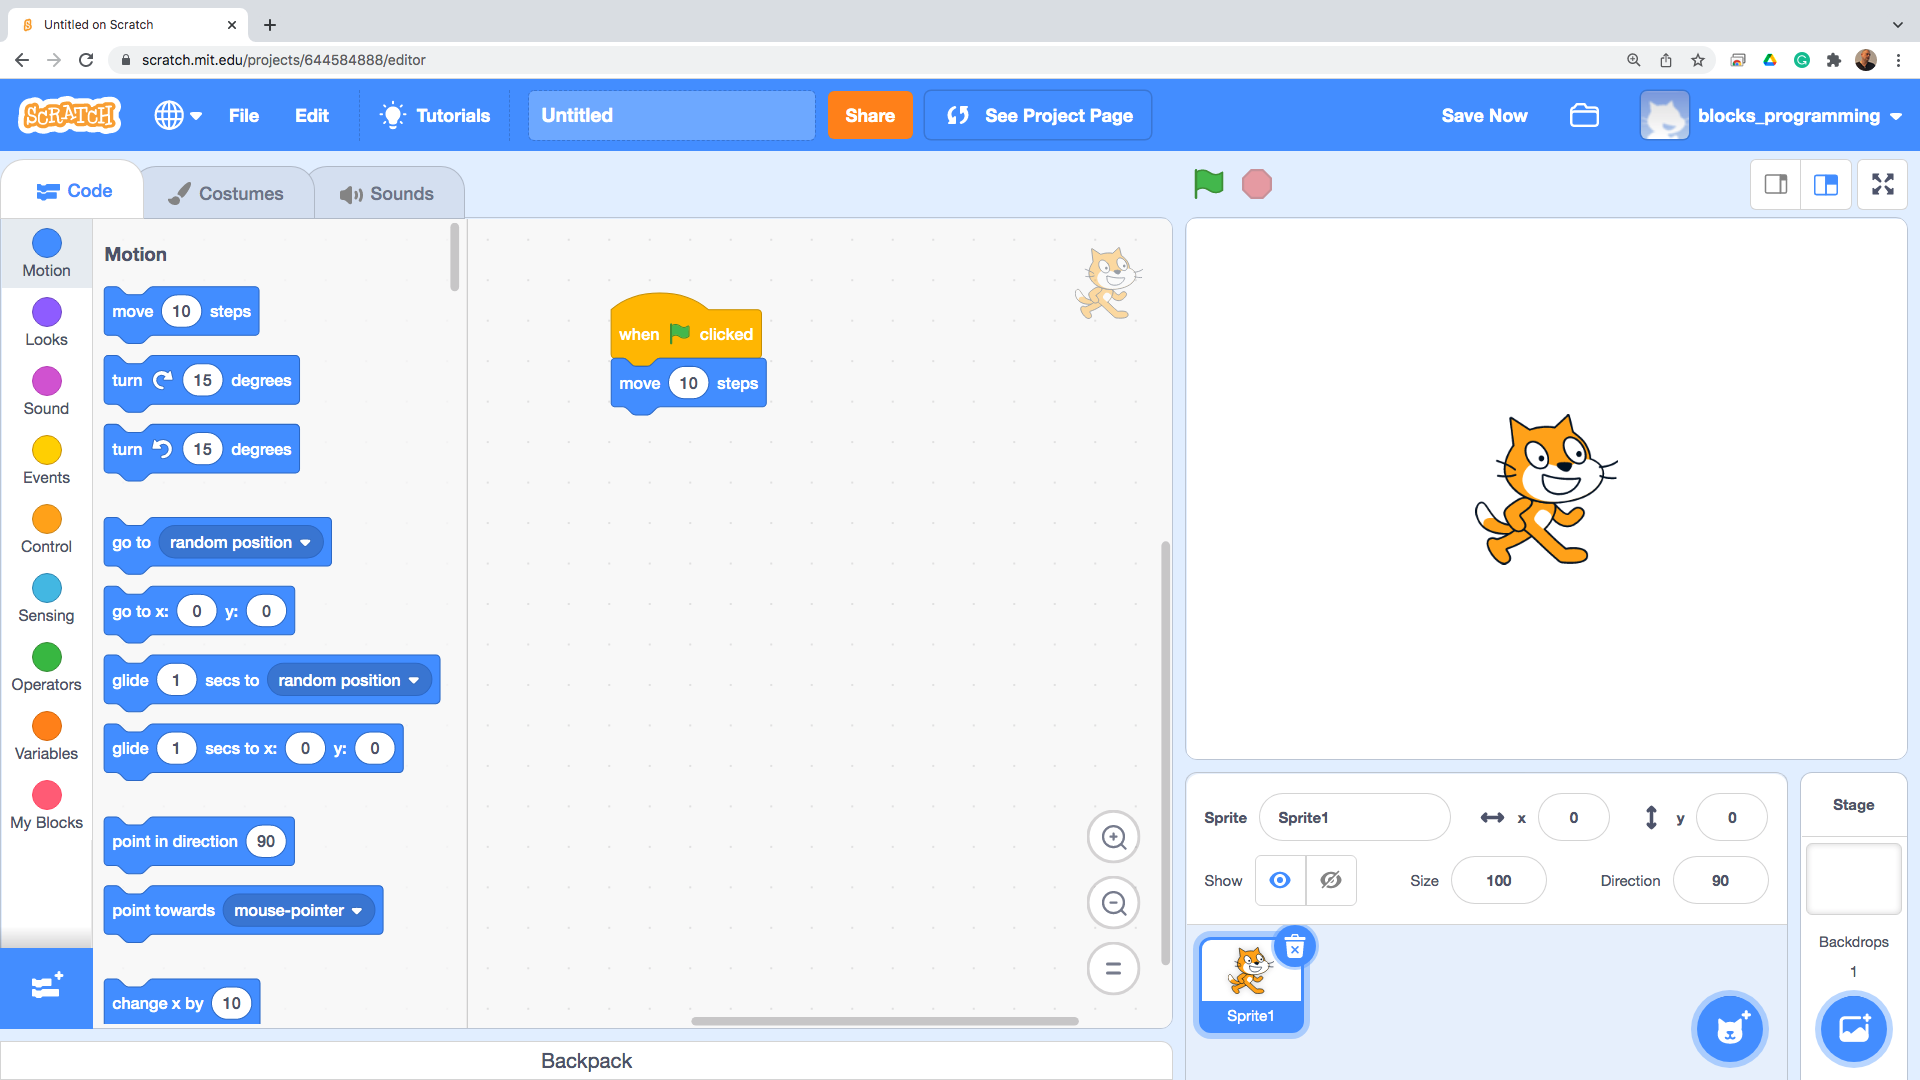
\includegraphics[width=1.0\linewidth,height=0.5\linewidth]{fig010014.png}
  \caption{Инструкция за придвижване на стъпки}
\label{fig010014}
\end{figure}

След преместването на котарака е от съществено значение да има една пауза на изчакване, така че визуално да се забележи преместването. За тази цел може да се приложи инструкция за изчакване, за определен брой секунди (Фиг. \ref{fig010015}).

\begin{figure}[H]
  \centering
  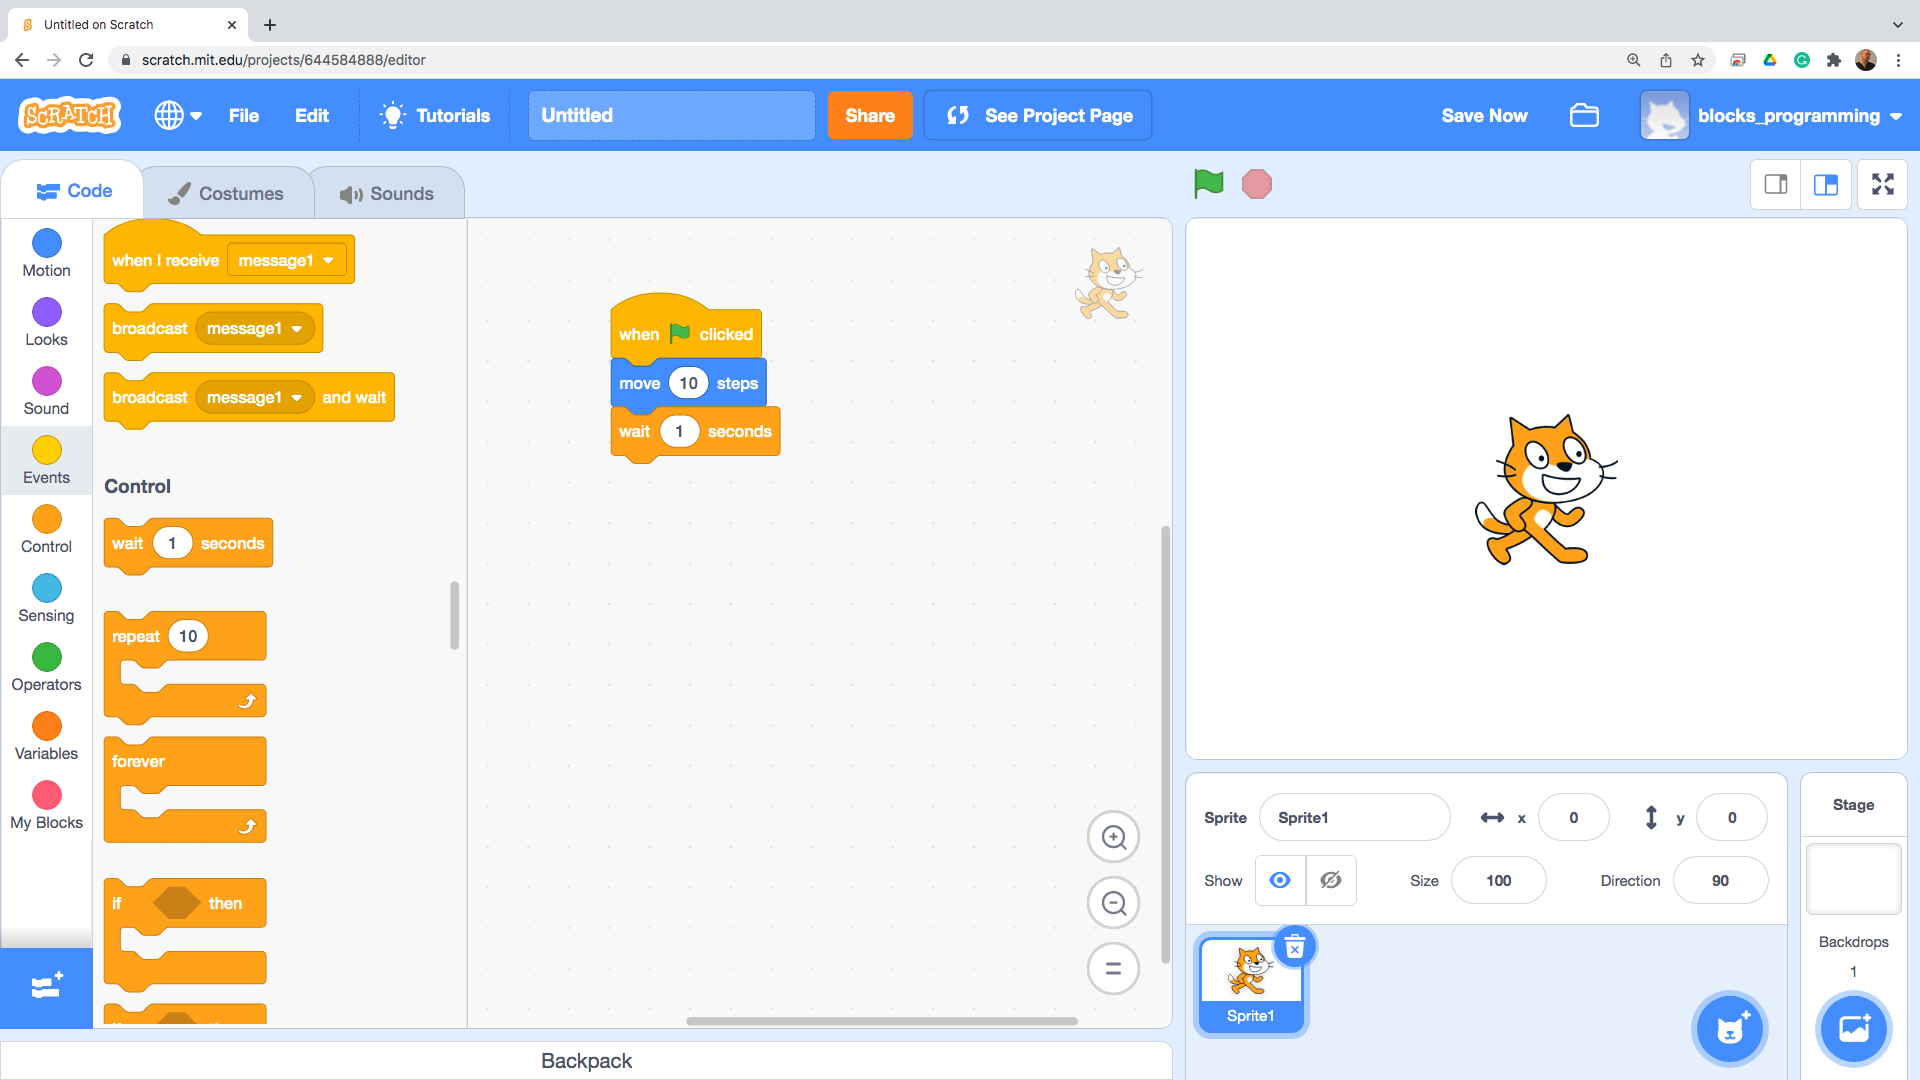
\includegraphics[width=1.0\linewidth,height=0.5\linewidth]{fig010015.png}
  \caption{Инструкция за изчакване}
\label{fig010015}
\end{figure}

След изчакването, котката може да се върне на първоначалната си позиция, като се изпълни инструкция за придвижване с отрицателен брой стъпки (Фиг. \ref{fig010016}).

\begin{figure}[H]
  \centering
  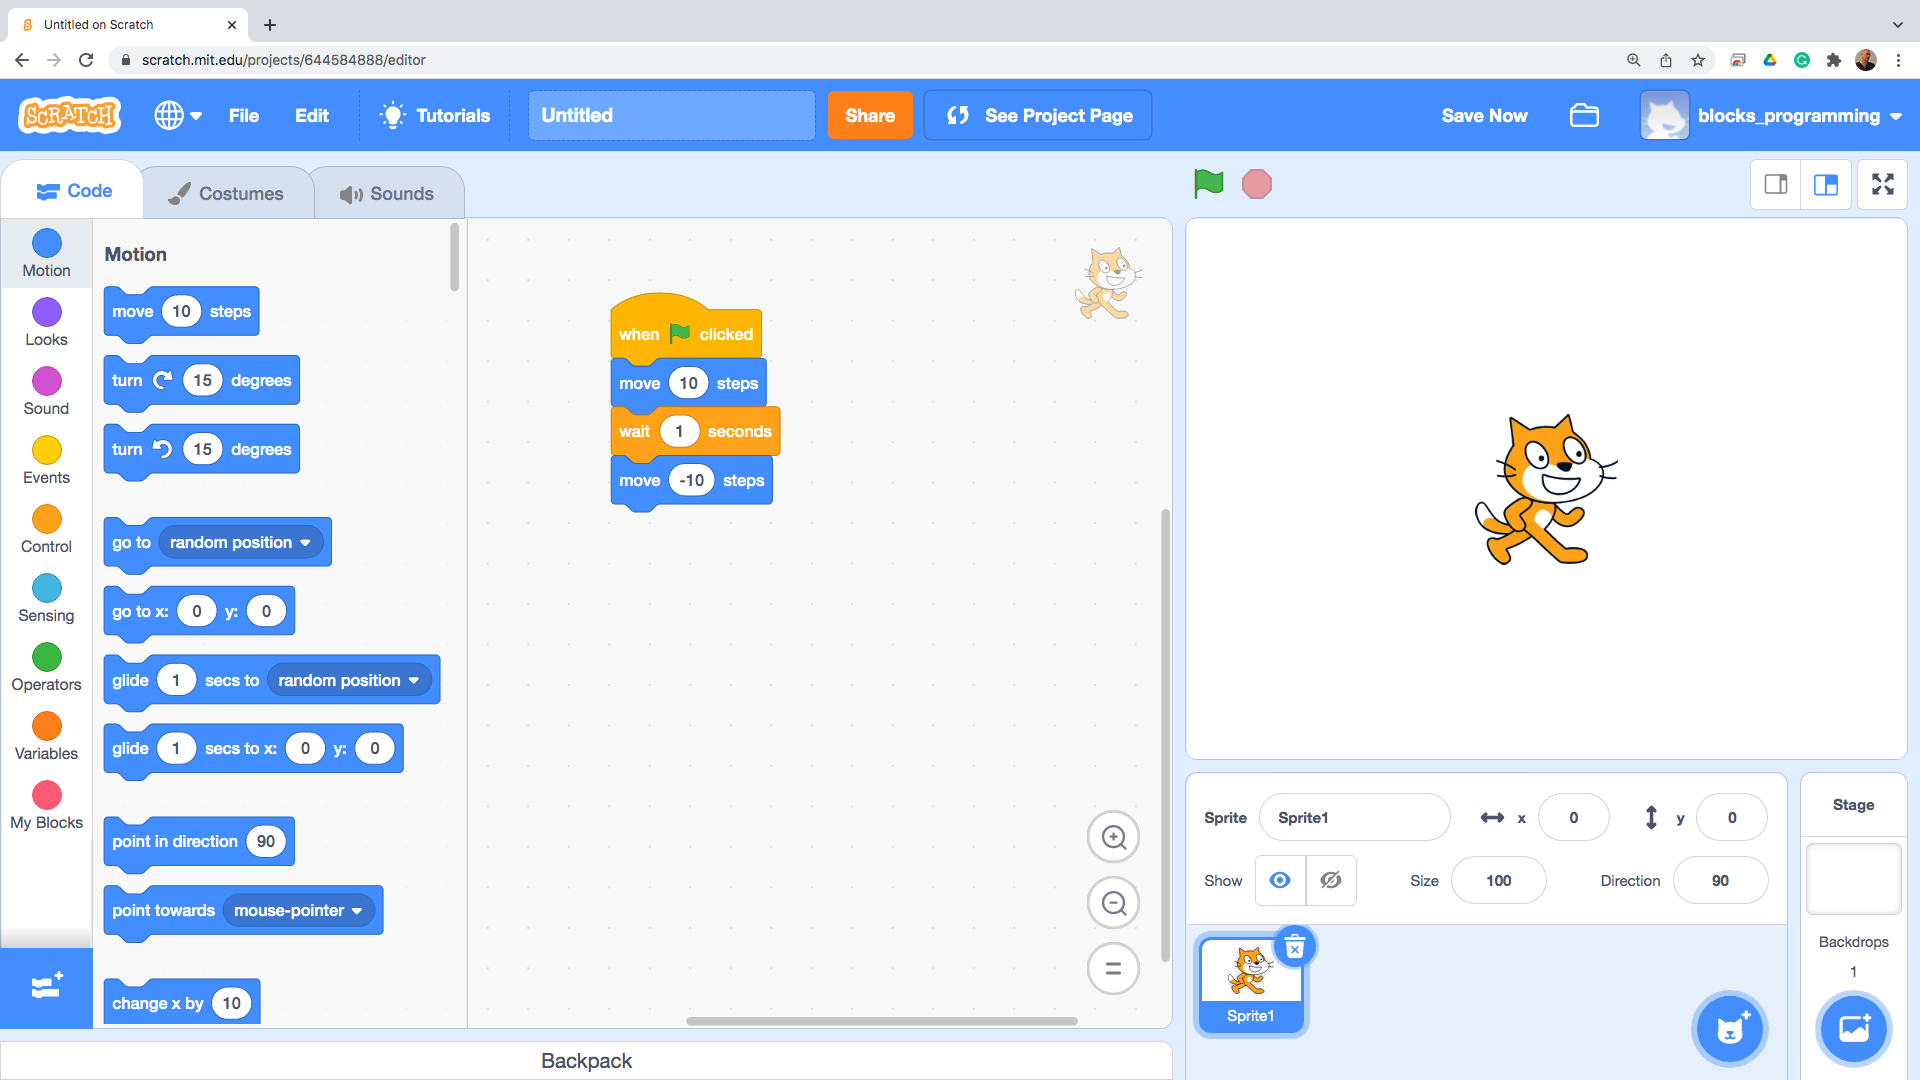
\includegraphics[width=1.0\linewidth,height=0.5\linewidth]{fig010016.png}
  \caption{Инструкция за преместване обратно}
\label{fig010016}
\end{figure}

След като всички предвидени инструкции са изпълнени е разумно да се сложи край на програмата, за което е предвидено отделно блокче в списъка с инструкции (Фиг. \ref{fig010017}).

\begin{figure}[H]
  \centering
  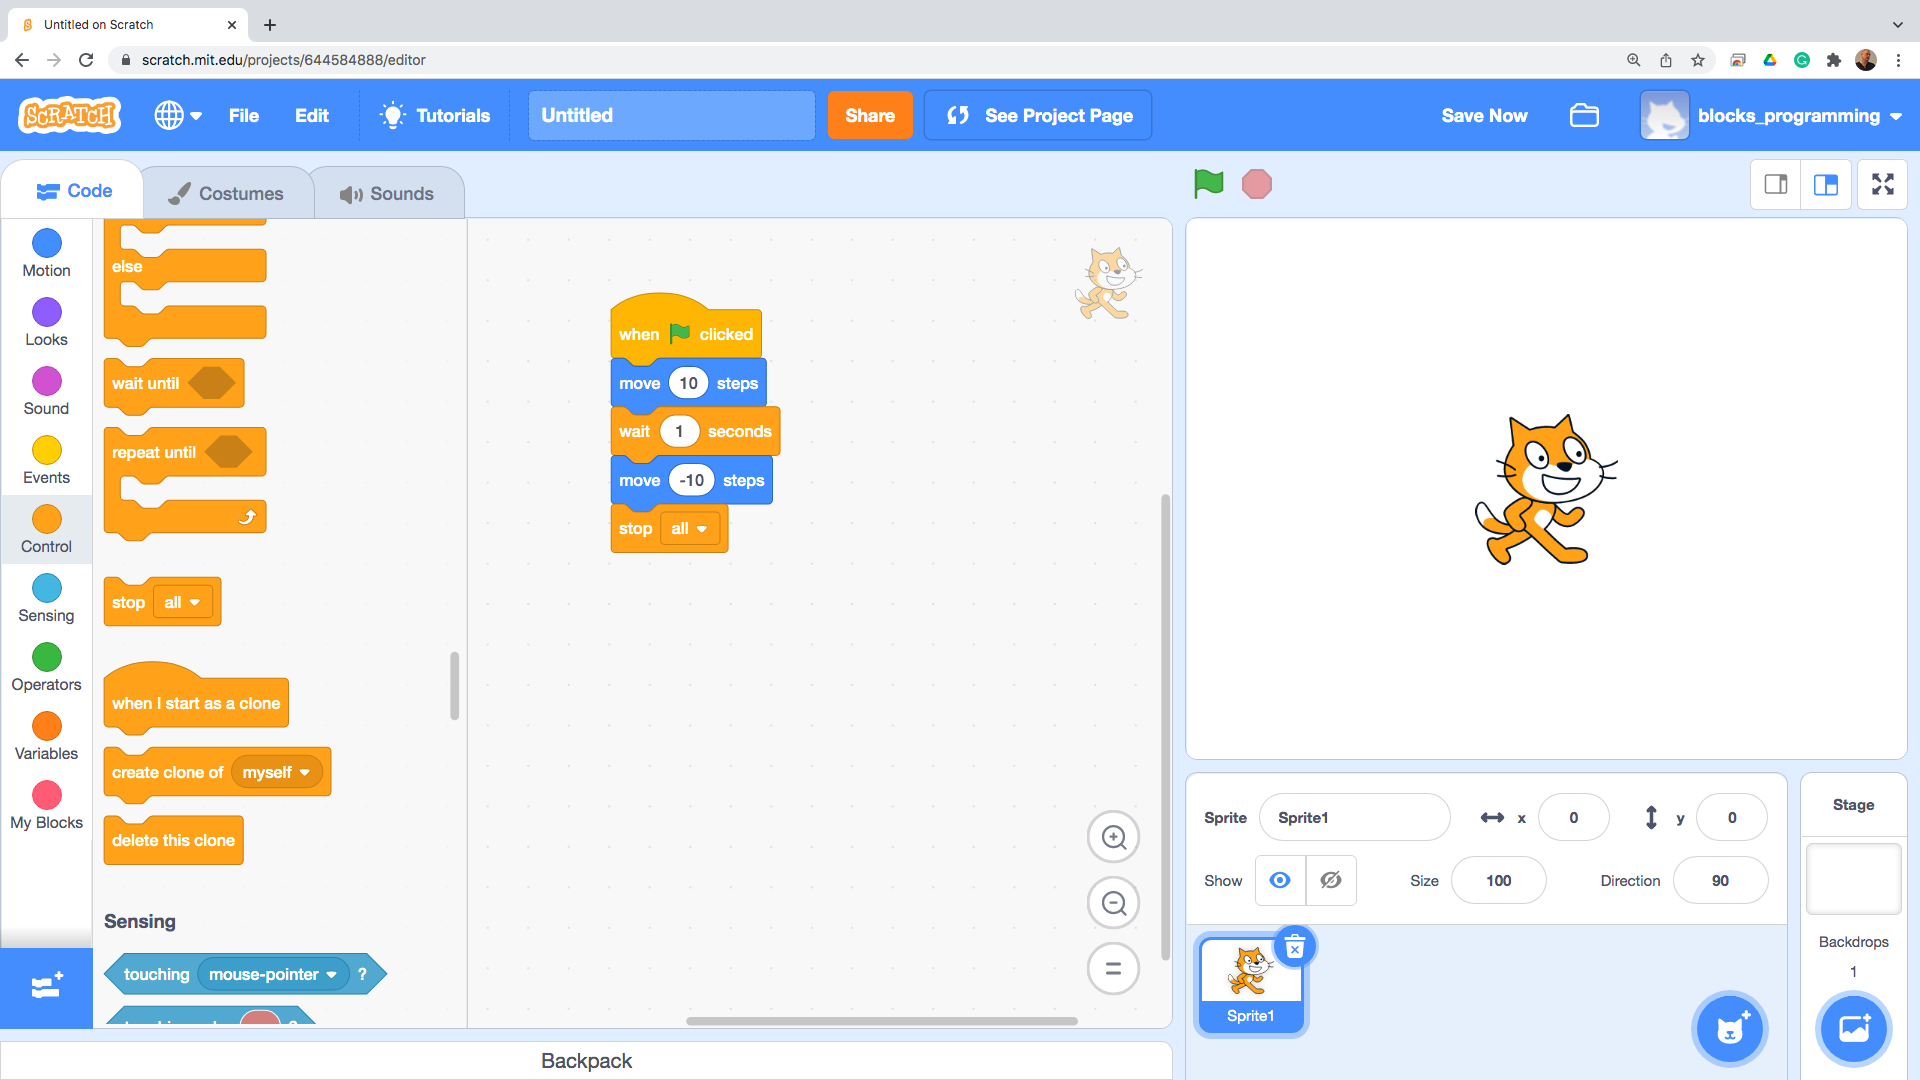
\includegraphics[width=1.0\linewidth,height=0.5\linewidth]{fig010017.png}
  \caption{Инструкция за край}
\label{fig010017}
\end{figure}

Така написаната програма се изпълнява, чрез натискане на зеления флаг (Фиг. \ref{fig010018}), а при нужда от аварийно спиране се натиска червеният кръг, от дясно на зеления флаг.

\begin{figure}[H]
  \centering
  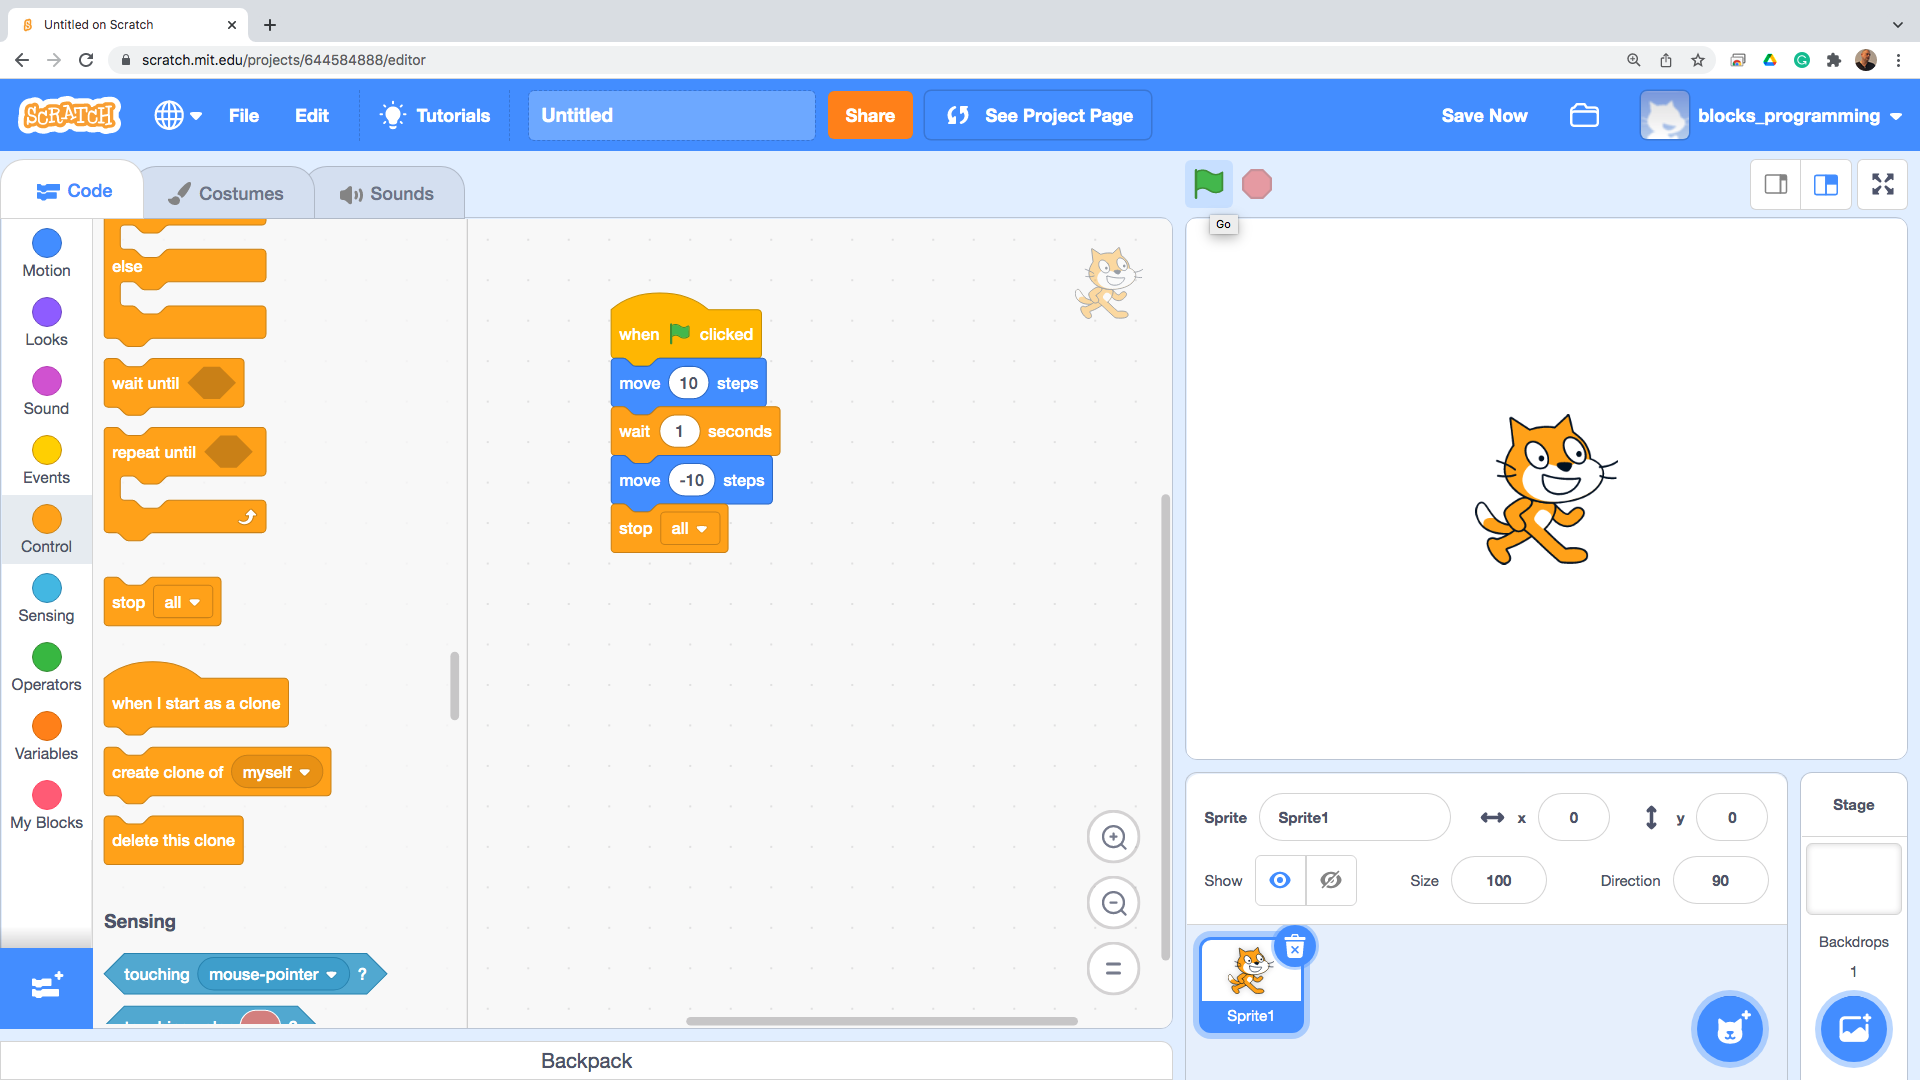
\includegraphics[width=1.0\linewidth,height=0.5\linewidth]{fig010018.png}
  \caption{Изпълнение на програмата}
\label{fig010018}
\end{figure}

Всяка програма, която се пише в Scratch се помества в отделен проект. Достъп до всички проекти на потребителя може да се получи от менюто „My Stuff“, което е част от списъка с опции за боравене с регистрирания потребител (Фиг. \ref{fig010019}).

\begin{figure}[H]
  \centering
  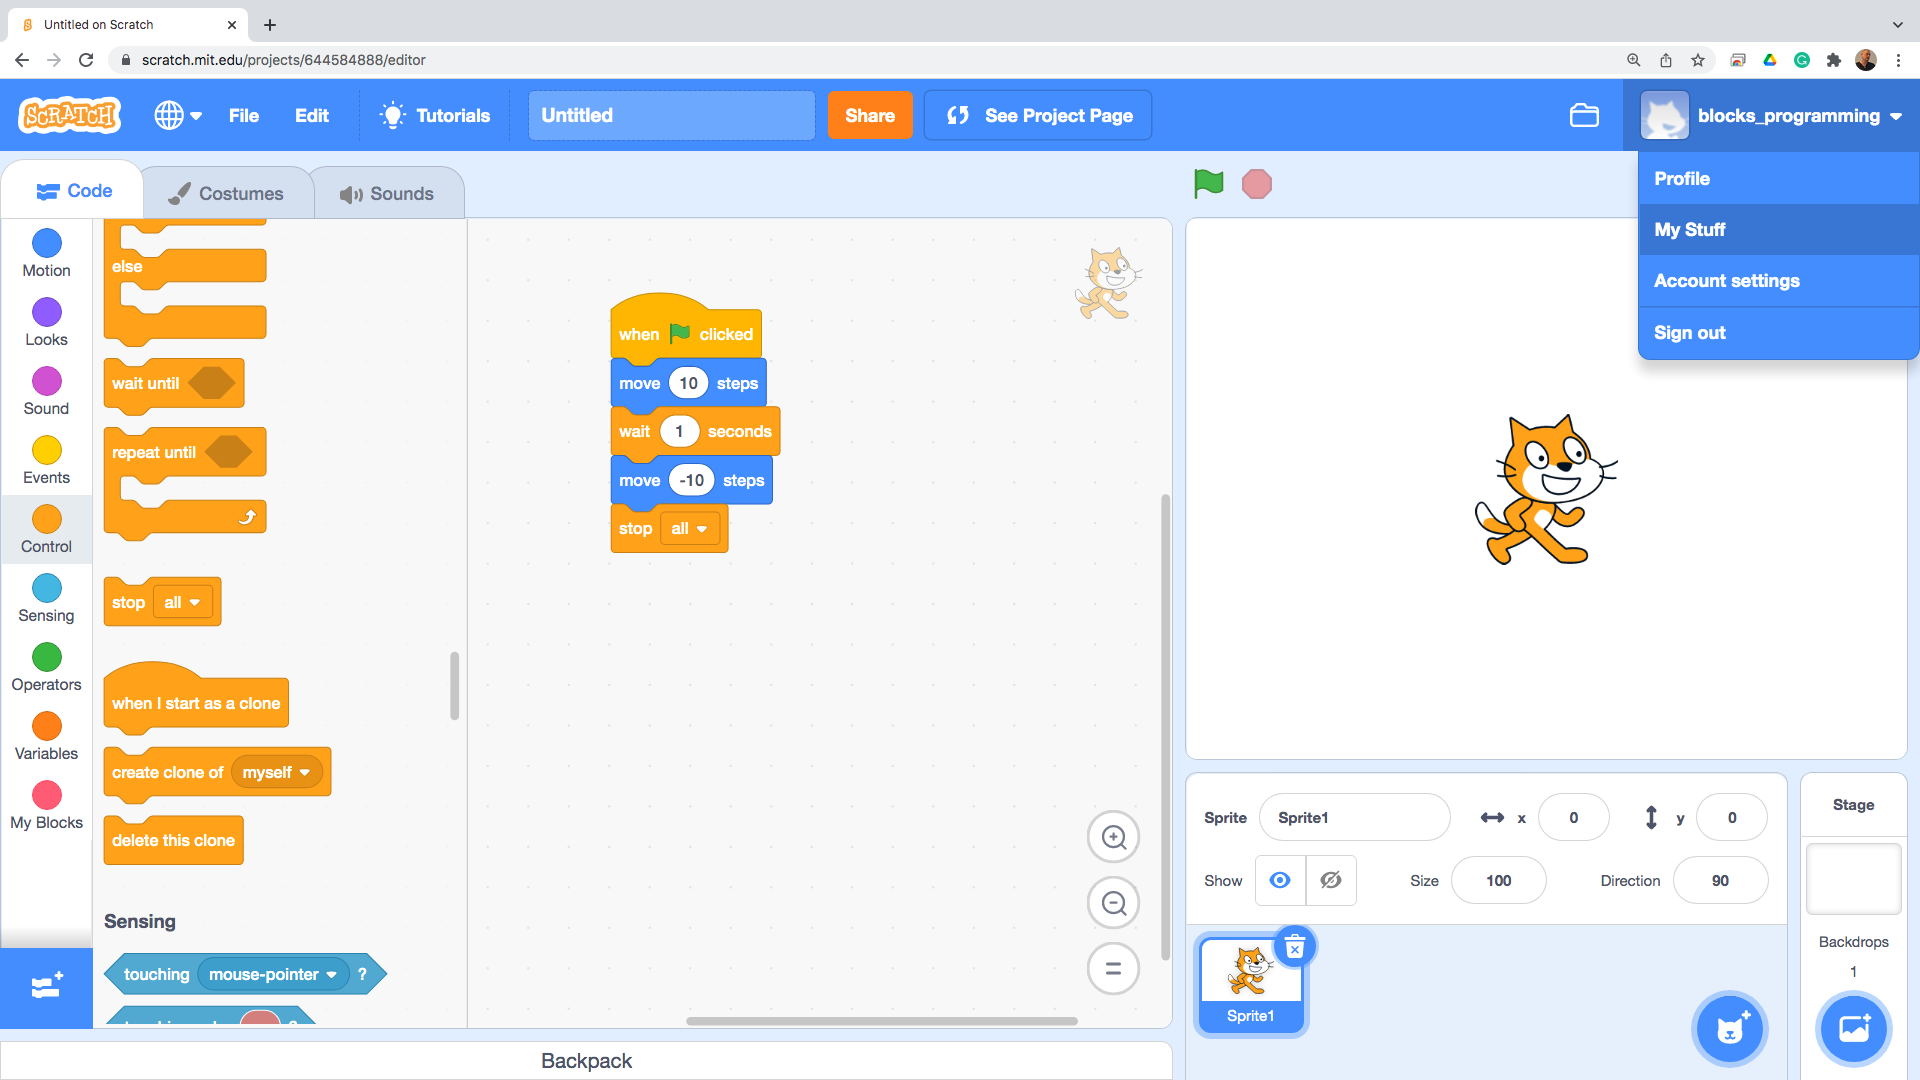
\includegraphics[width=1.0\linewidth,height=0.5\linewidth]{fig010019.png}
  \caption{Меню за организация на проектите}
\label{fig010019}
\end{figure}

Първоначално, всеки проект има служебно име (Фиг. \ref{fig010020}), което в последствие може да бъде променено. Едно от най-атрактивните предимства на програмната среда е, че проектите на потребителите могат да се споделят (Sharing) с много широка аудитория. Това позволява бърз трансфер на знания и умения, както и оценка за положения труд. 

\begin{figure}[H]
  \centering
  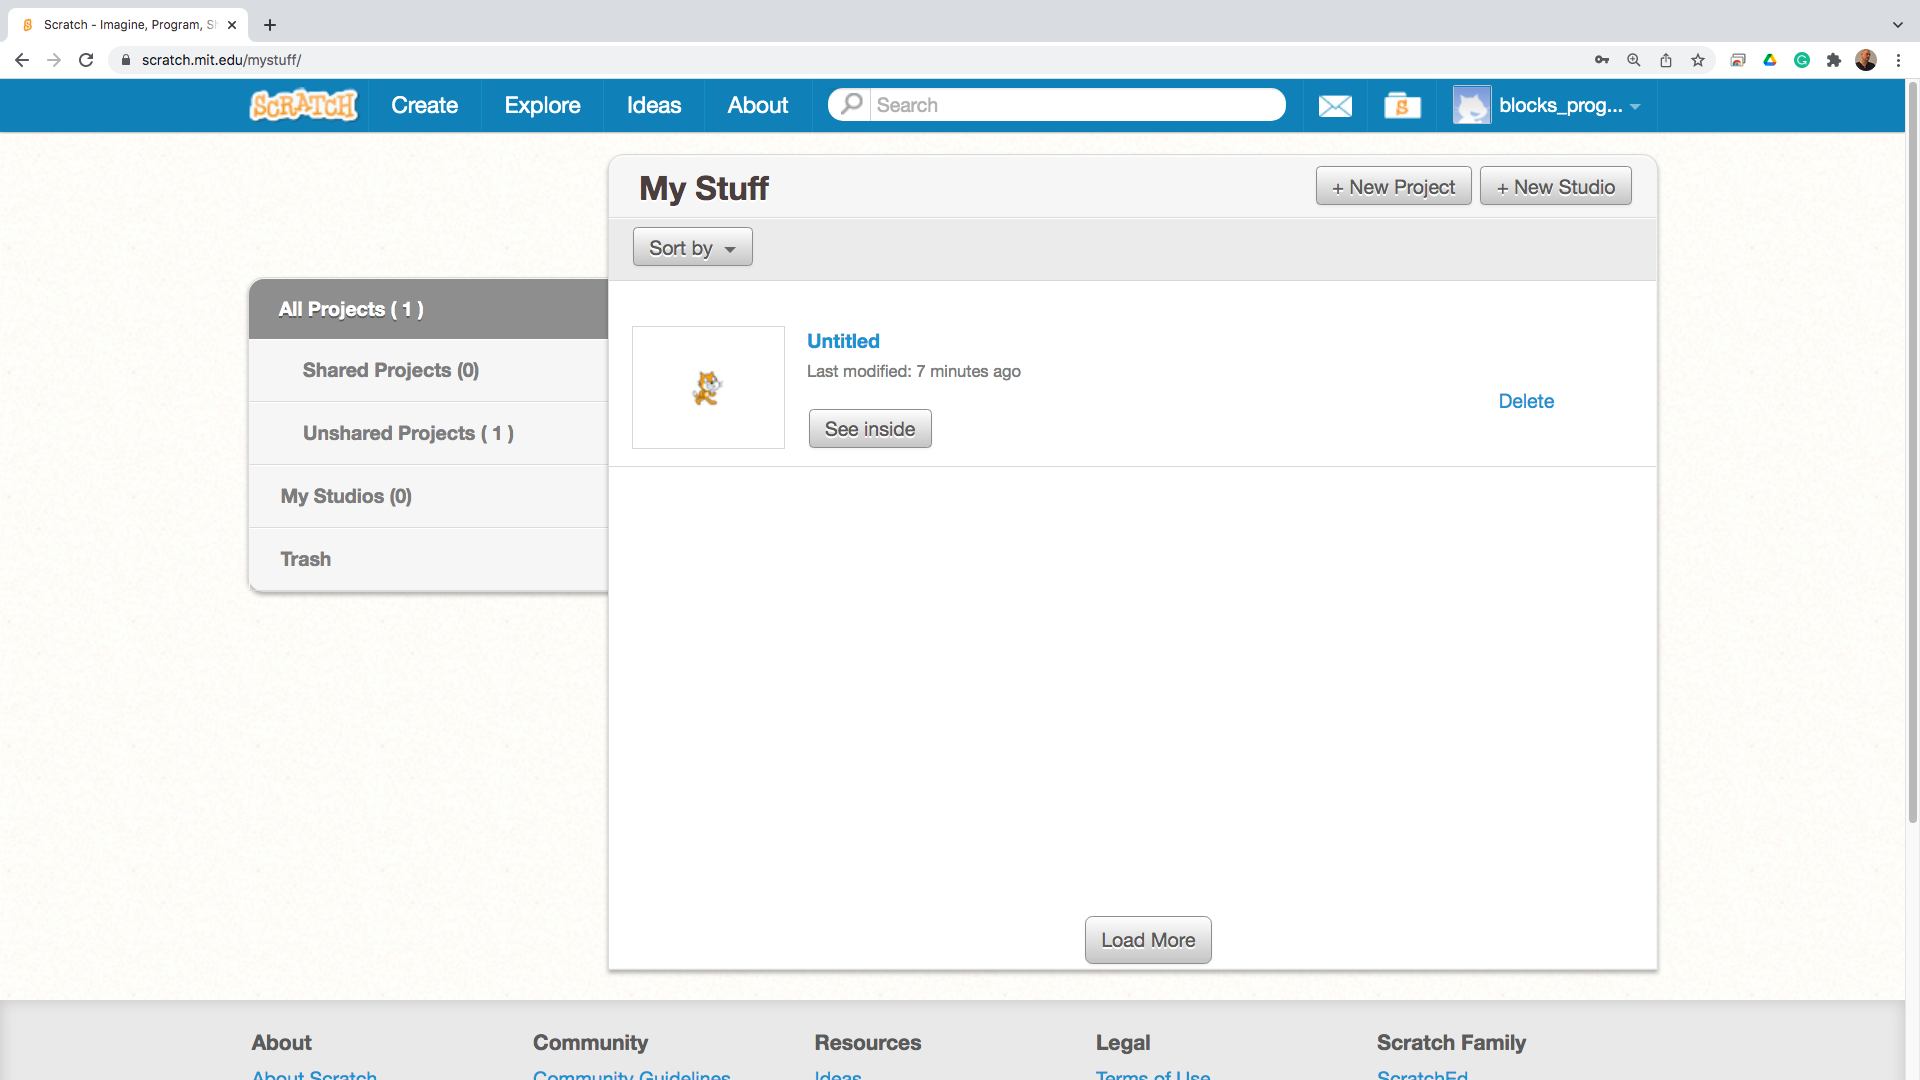
\includegraphics[width=1.0\linewidth,height=0.5\linewidth]{fig010020.png}
  \caption{Списък с проекти}
\label{fig010020}
\end{figure}

Най-голямото очарование блоковите езици получават от факта, че писането на инструкциите и формирането на цялостна програма прилича на подреждането на пъзел. Почти всички деца обичат да редят пазели. Харесват ярките цветове и красивите картини. Когато чарът на класическите пъзели се пренесе в една толкова атрактивна област, каквато е програмирането, резултатите могат да бъдат смайващи. 

\section{Първи стъпки в App Inventor}

Работата в средата на App Inventor започва със зареждане на главната уеб страница (Фиг. \ref{fig010021}), която се намира на адрес: \\ \href{https://appinventor.mit.edu/}{https://appinventor.mit.edu/}

\begin{figure}[H]
  \centering
  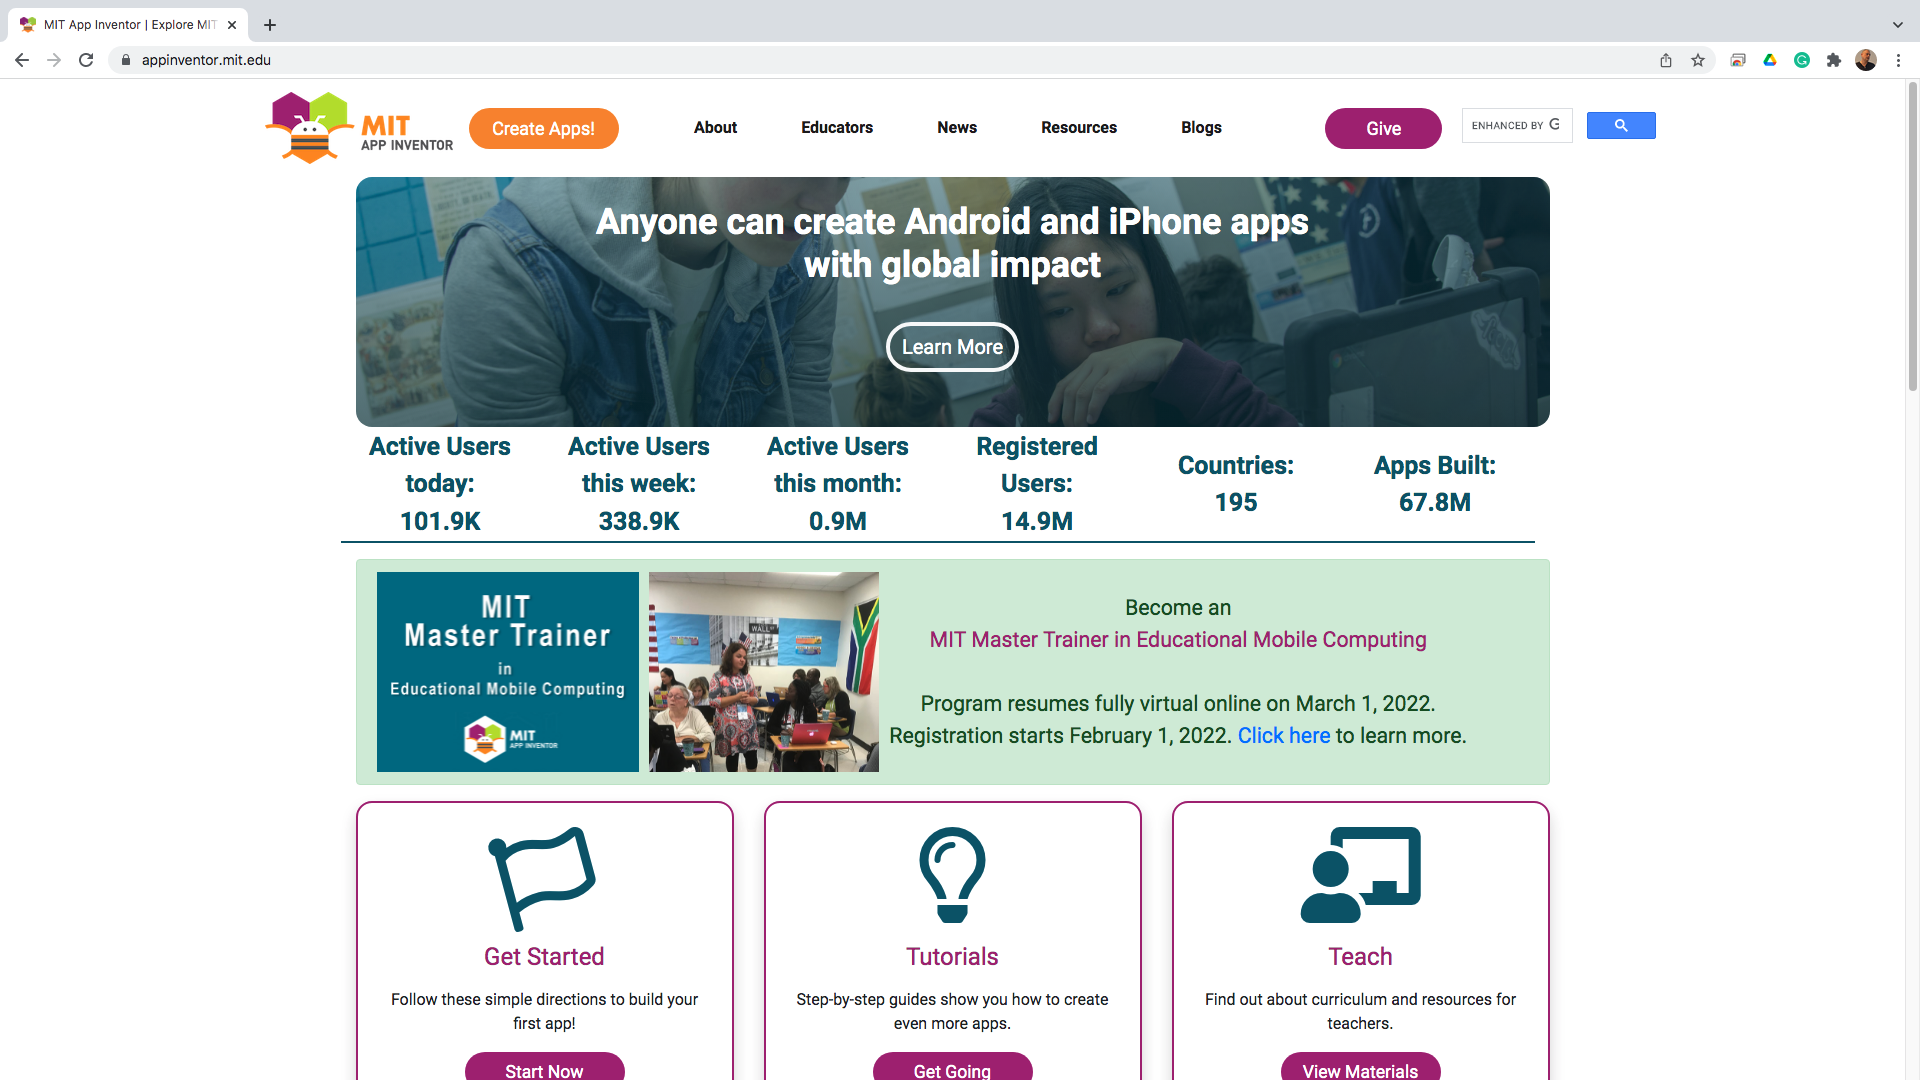
\includegraphics[width=1.0\linewidth,height=0.5\linewidth]{fig010021.png}
  \caption{Начална уеб страница на App Inventor}
\label{fig010021}
\end{figure}

Въпреки че App Inventor също е продукт на Масачузетския технологичен институт в някои аспекти работата с него се различава от начина по който се работи в Scratch. App Inventor също се предлага под формата на облачна услуга в която е необходима регистрация. За разлика от  Scratch, в App Inventor може да се пропусне създаването на потребителски профил, а влизането в системата да се осъществи, чрез класическа регистрация в услугата GMail. Този процес започва след избирането на оранжевия бутон „Create Apps!“ (Фиг. \ref{fig010022}).

\begin{figure}[H]
  \centering
  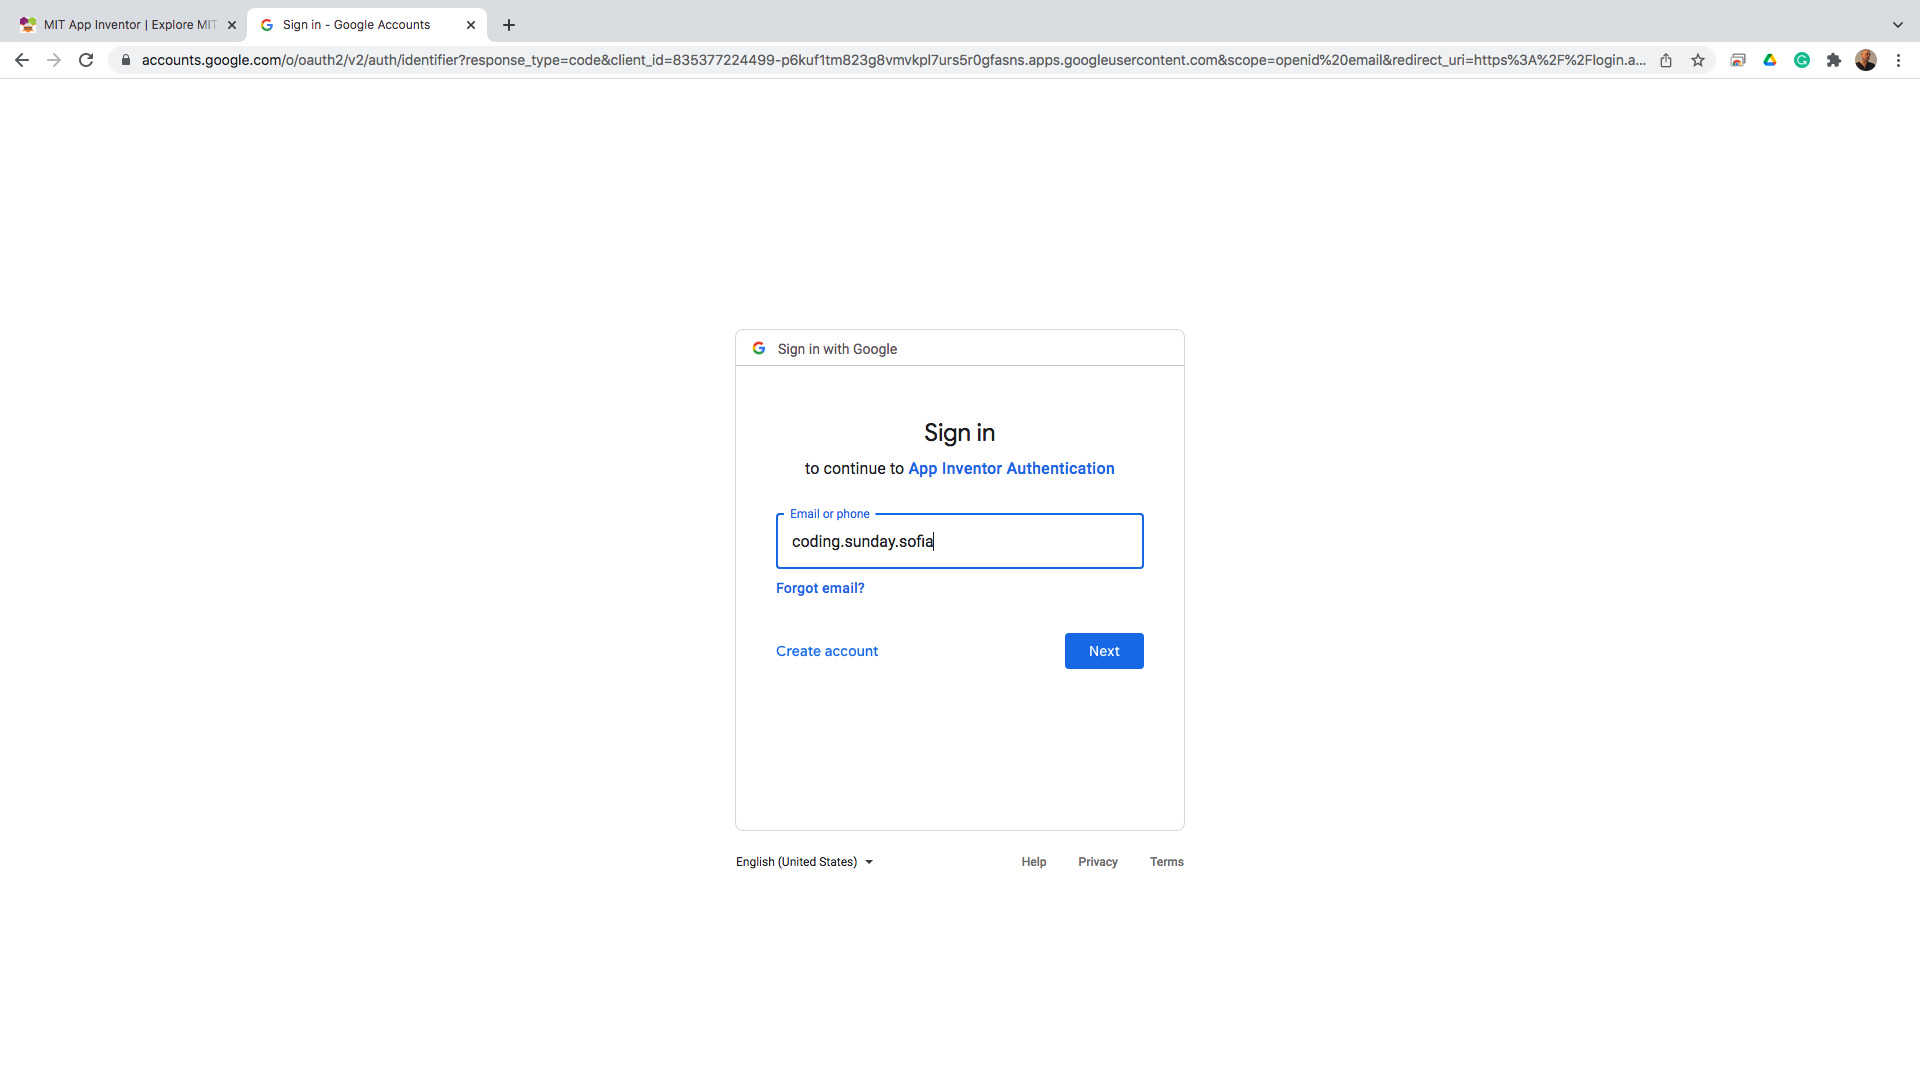
\includegraphics[width=1.0\linewidth,height=0.5\linewidth]{fig010022.png}
  \caption{Избор на GMail потребител за включване в системата}
\label{fig010022}
\end{figure}

След избора на потребител, с който да се работи в средата на App Inventor е нужно този потребител да се автентифицира, чрез въвеждане на парола (Фиг. \ref{fig010023}).

\begin{figure}[H]
  \centering
  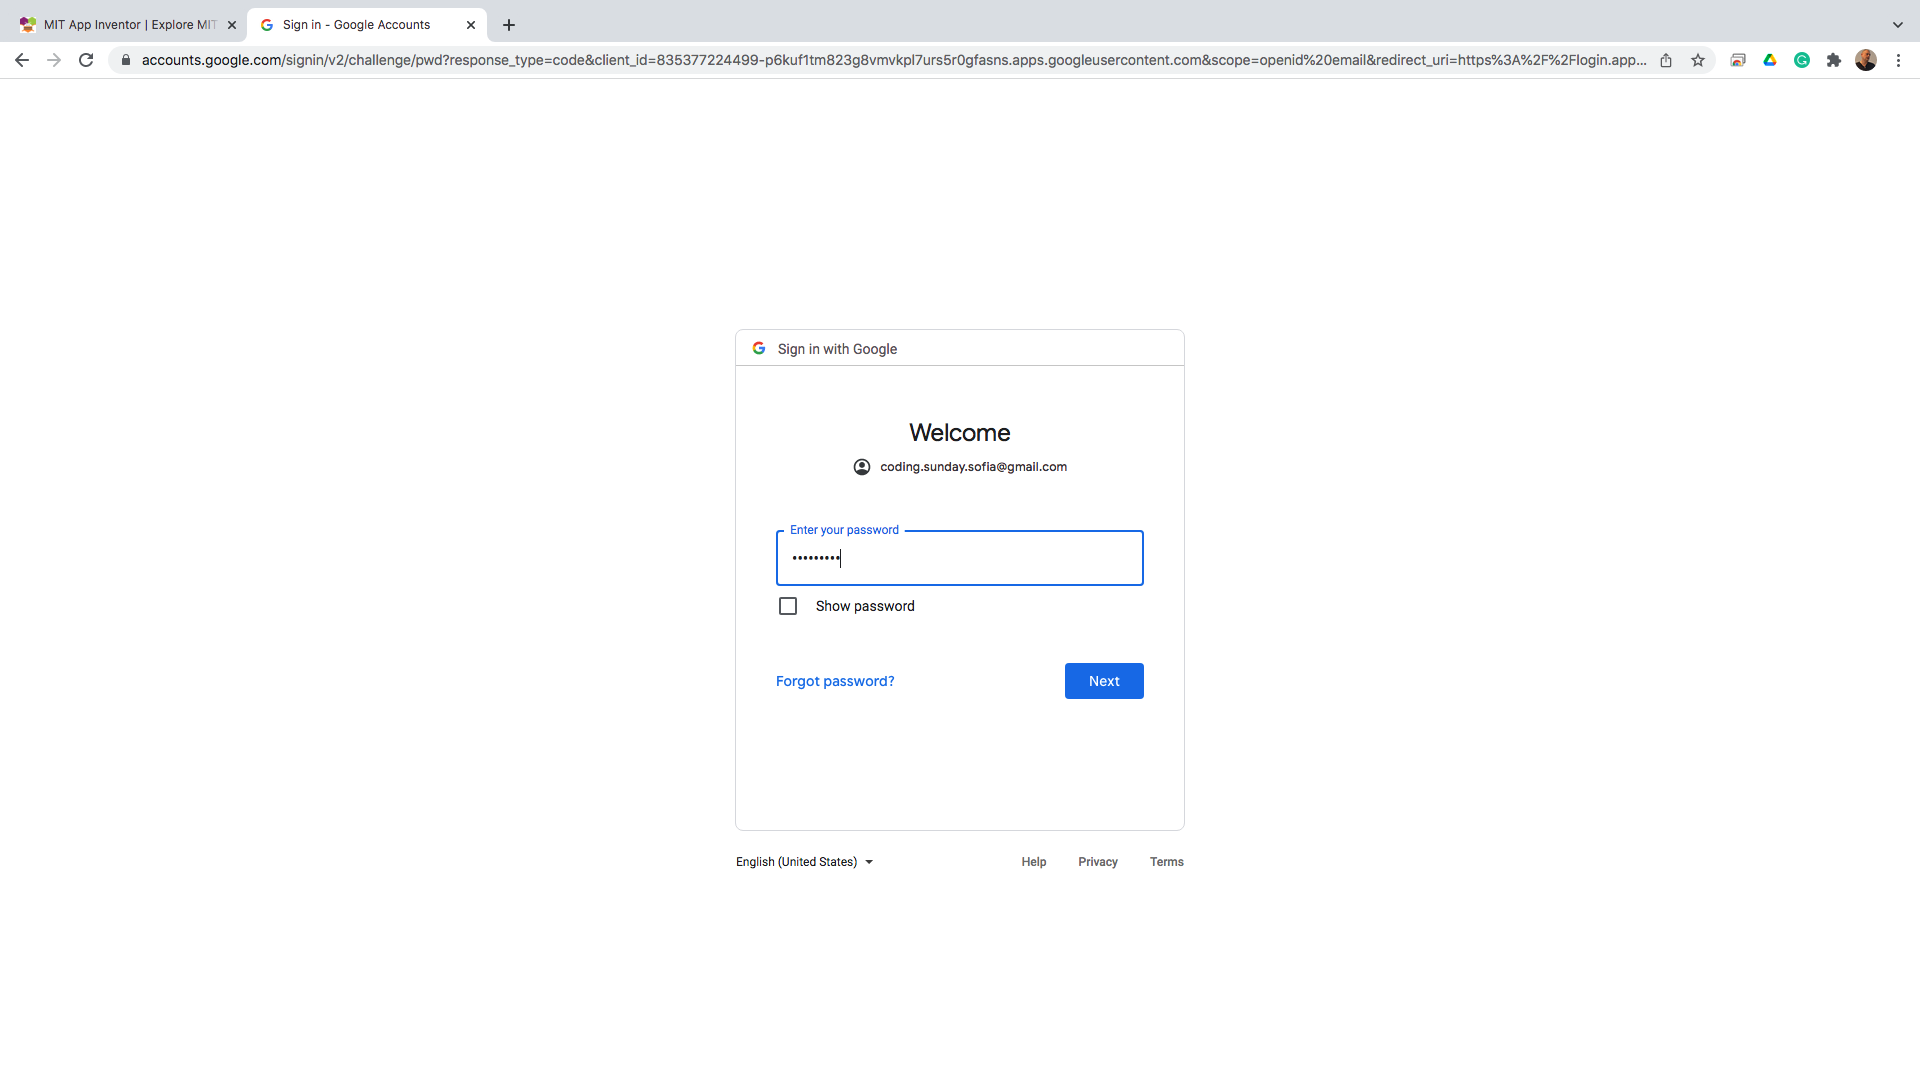
\includegraphics[width=1.0\linewidth,height=0.5\linewidth]{fig010023.png}
  \caption{Автентификация на потребителя}
\label{fig010023}
\end{figure}

За да бъде позволена работа в програмната среда на App Inventor се изисква съгласие от потребителя с общите условия на платформата (Фиг. \ref{fig010024}).

\begin{figure}[H]
  \centering
  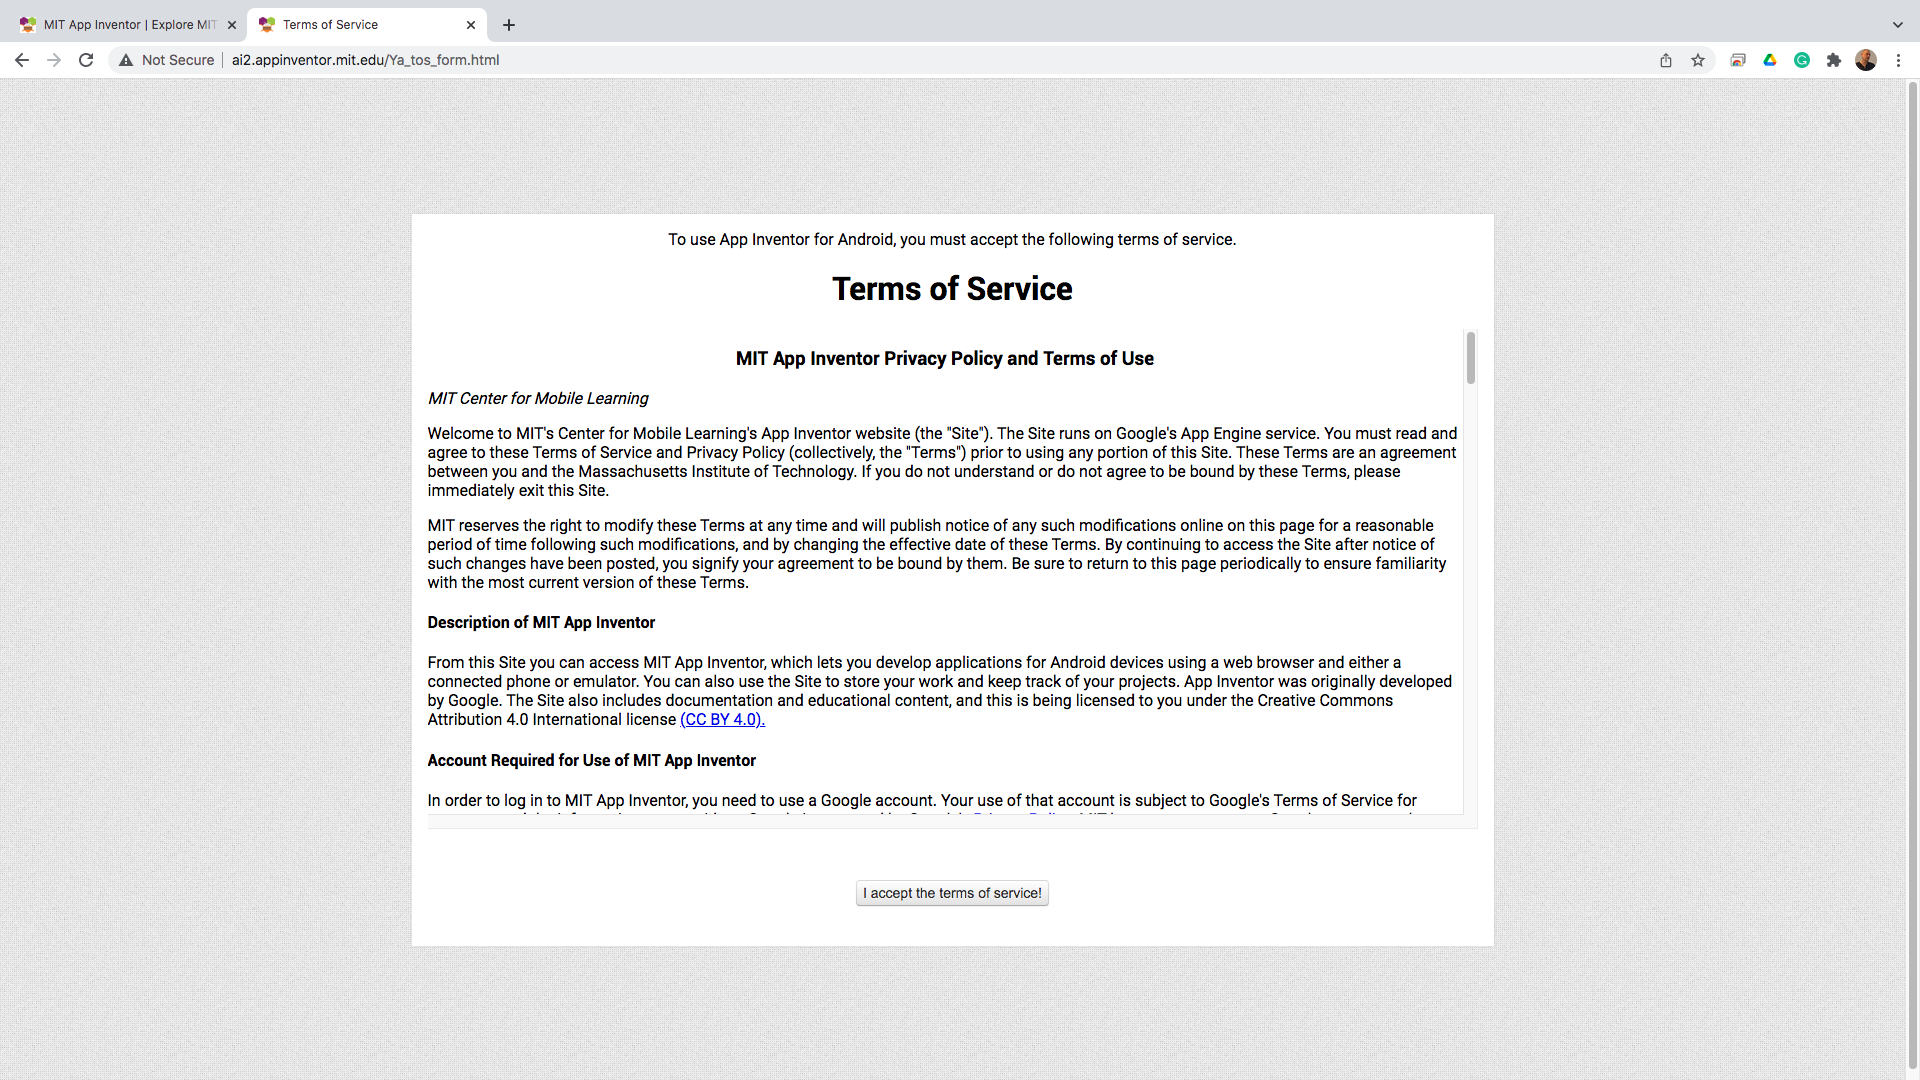
\includegraphics[width=1.0\linewidth,height=0.5\linewidth]{fig010024.png}
  \caption{Общи условия за ползване на програмната среда}
\label{fig010024}
\end{figure}

Процесът по вход в програмната среда завършва с поздравителна уеб страница (Фиг. \ref{fig010025}). На тази страница е представена по-подробна информация за програмната среда, видът на стартираната инстанция и версия. 

\begin{figure}[H]
  \centering
  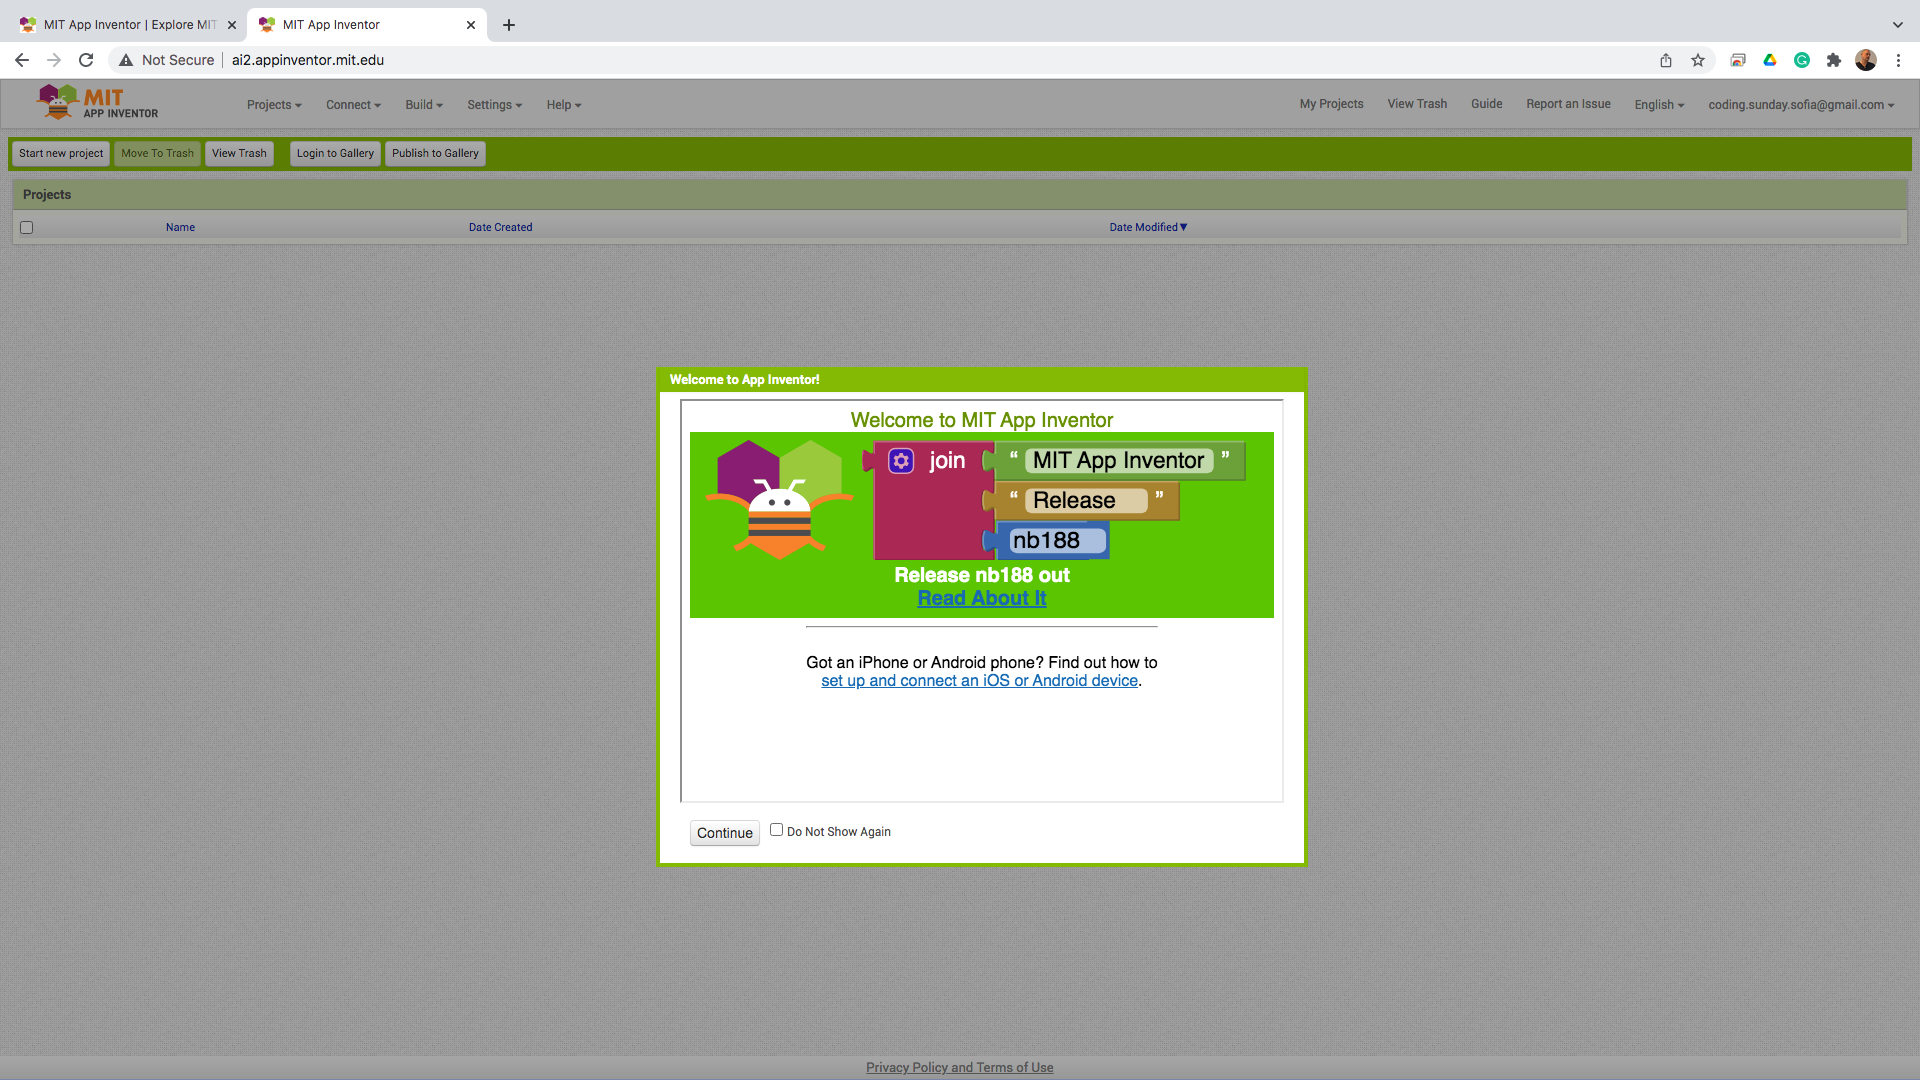
\includegraphics[width=1.0\linewidth,height=0.5\linewidth]{fig010025.png}
  \caption{Поздравителна страница}
\label{fig010025}
\end{figure}

Първата възможност, която се предлага на потребителя е да избере от възможности за разглеждане на няколко учебни проекта, служещи за първоначално въвеждане в начина за работа с програмната среда (Фиг. \ref{fig010026}).

\begin{figure}[H]
  \centering
  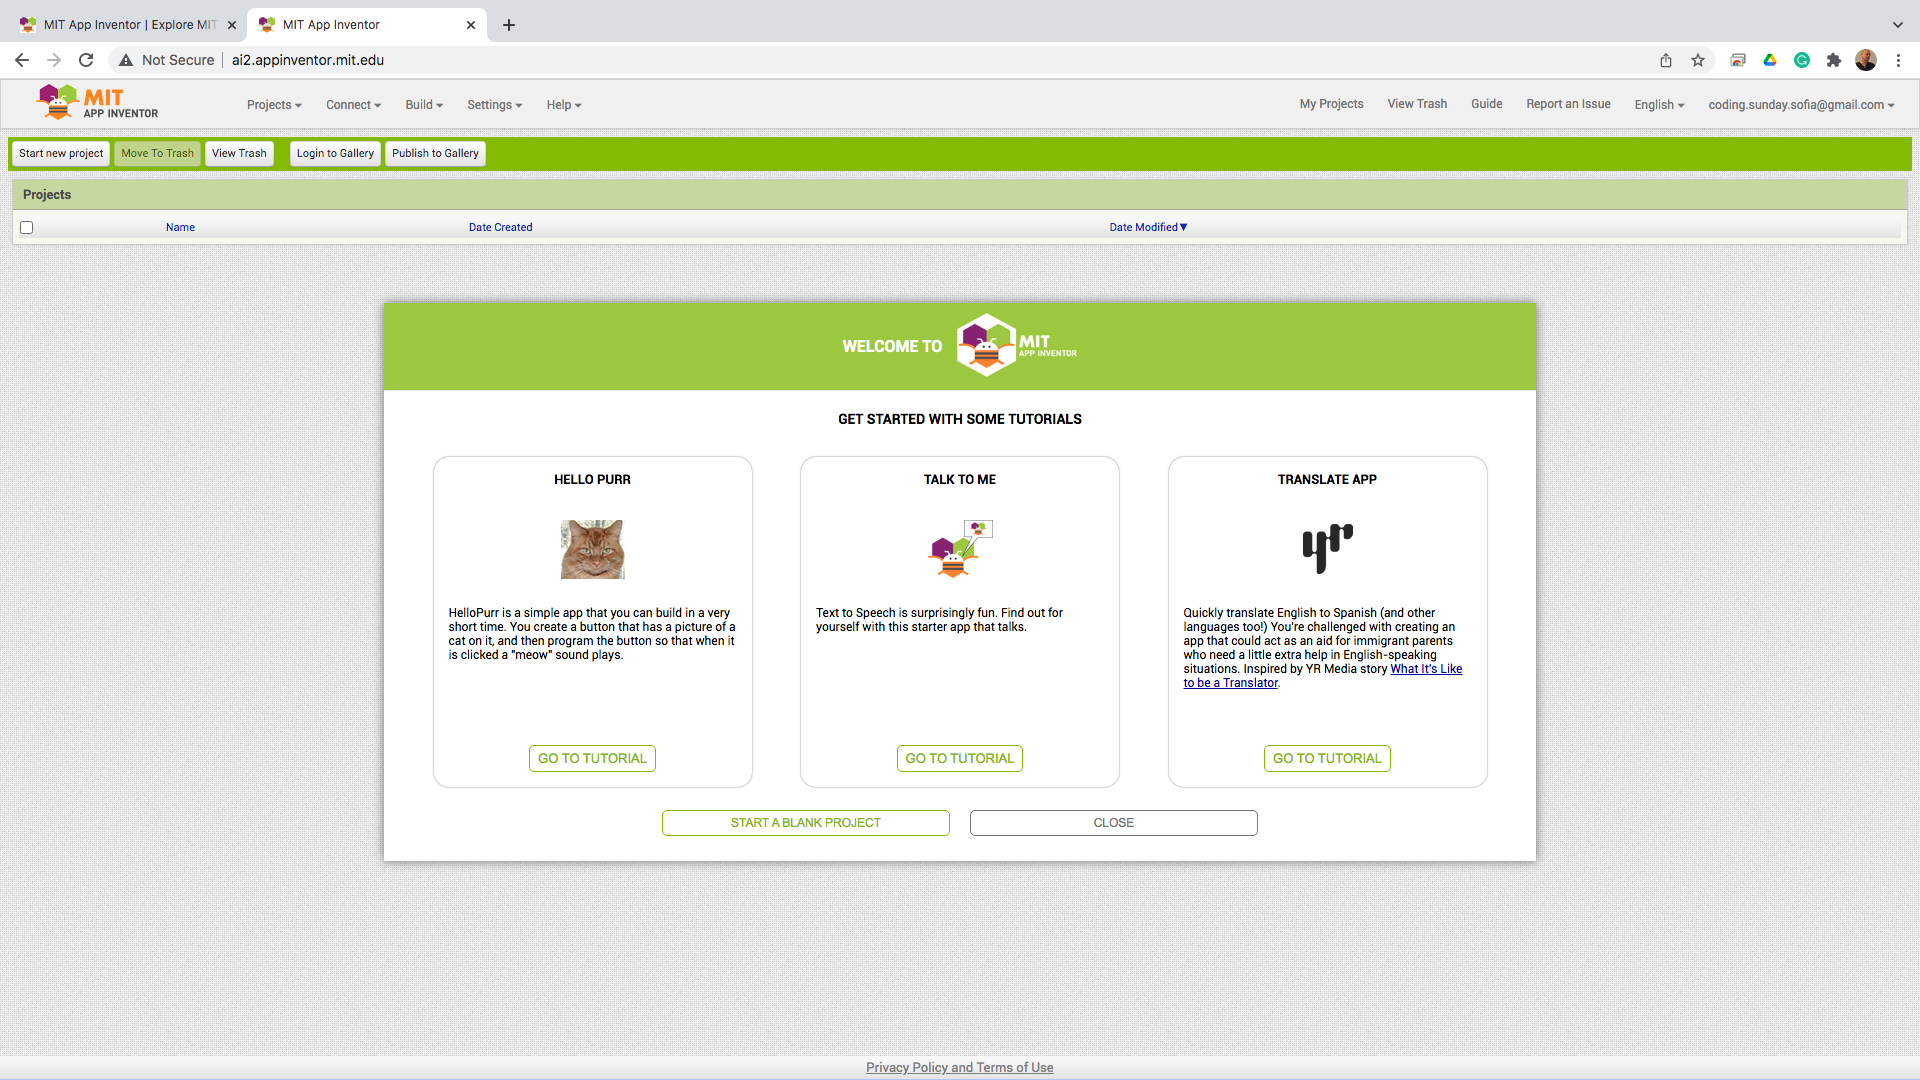
\includegraphics[width=1.0\linewidth,height=0.5\linewidth]{fig010026.png}
  \caption{Възможност за избор на учебни проекти}
\label{fig010026}
\end{figure}

Ако не бъде избран учебен проект или опцията за създаване на празен проект, системата насочва потребителя към страницата със списък от собствени проекти (Фиг. \ref{fig010027}).

\begin{figure}[H]
  \centering
  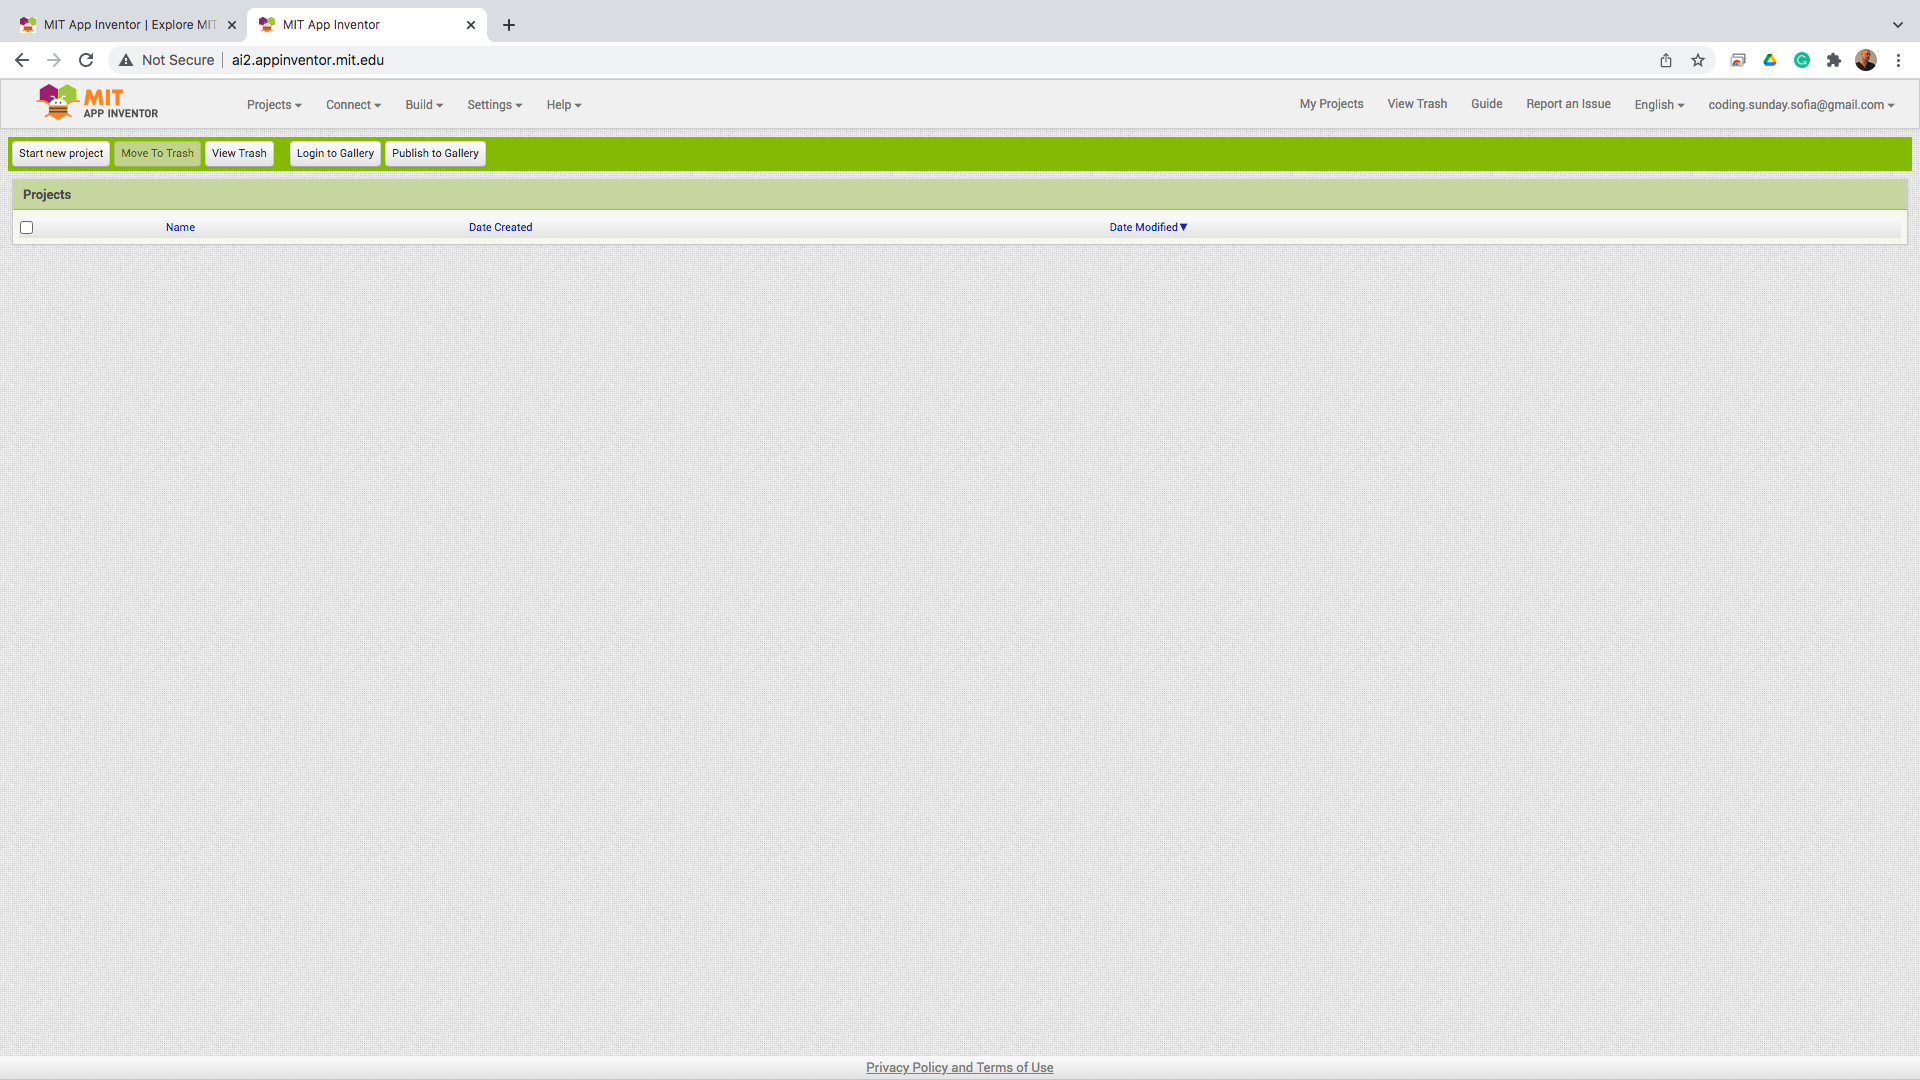
\includegraphics[width=1.0\linewidth,height=0.5\linewidth]{fig010027.png}
  \caption{Страница със списък от собствени проекти}
\label{fig010027}
\end{figure}

Започването на нов проект се случва от бутон, горе в ляво, на основният работен екран (Фиг. \ref{fig010028}).

\begin{figure}[H]
  \centering
  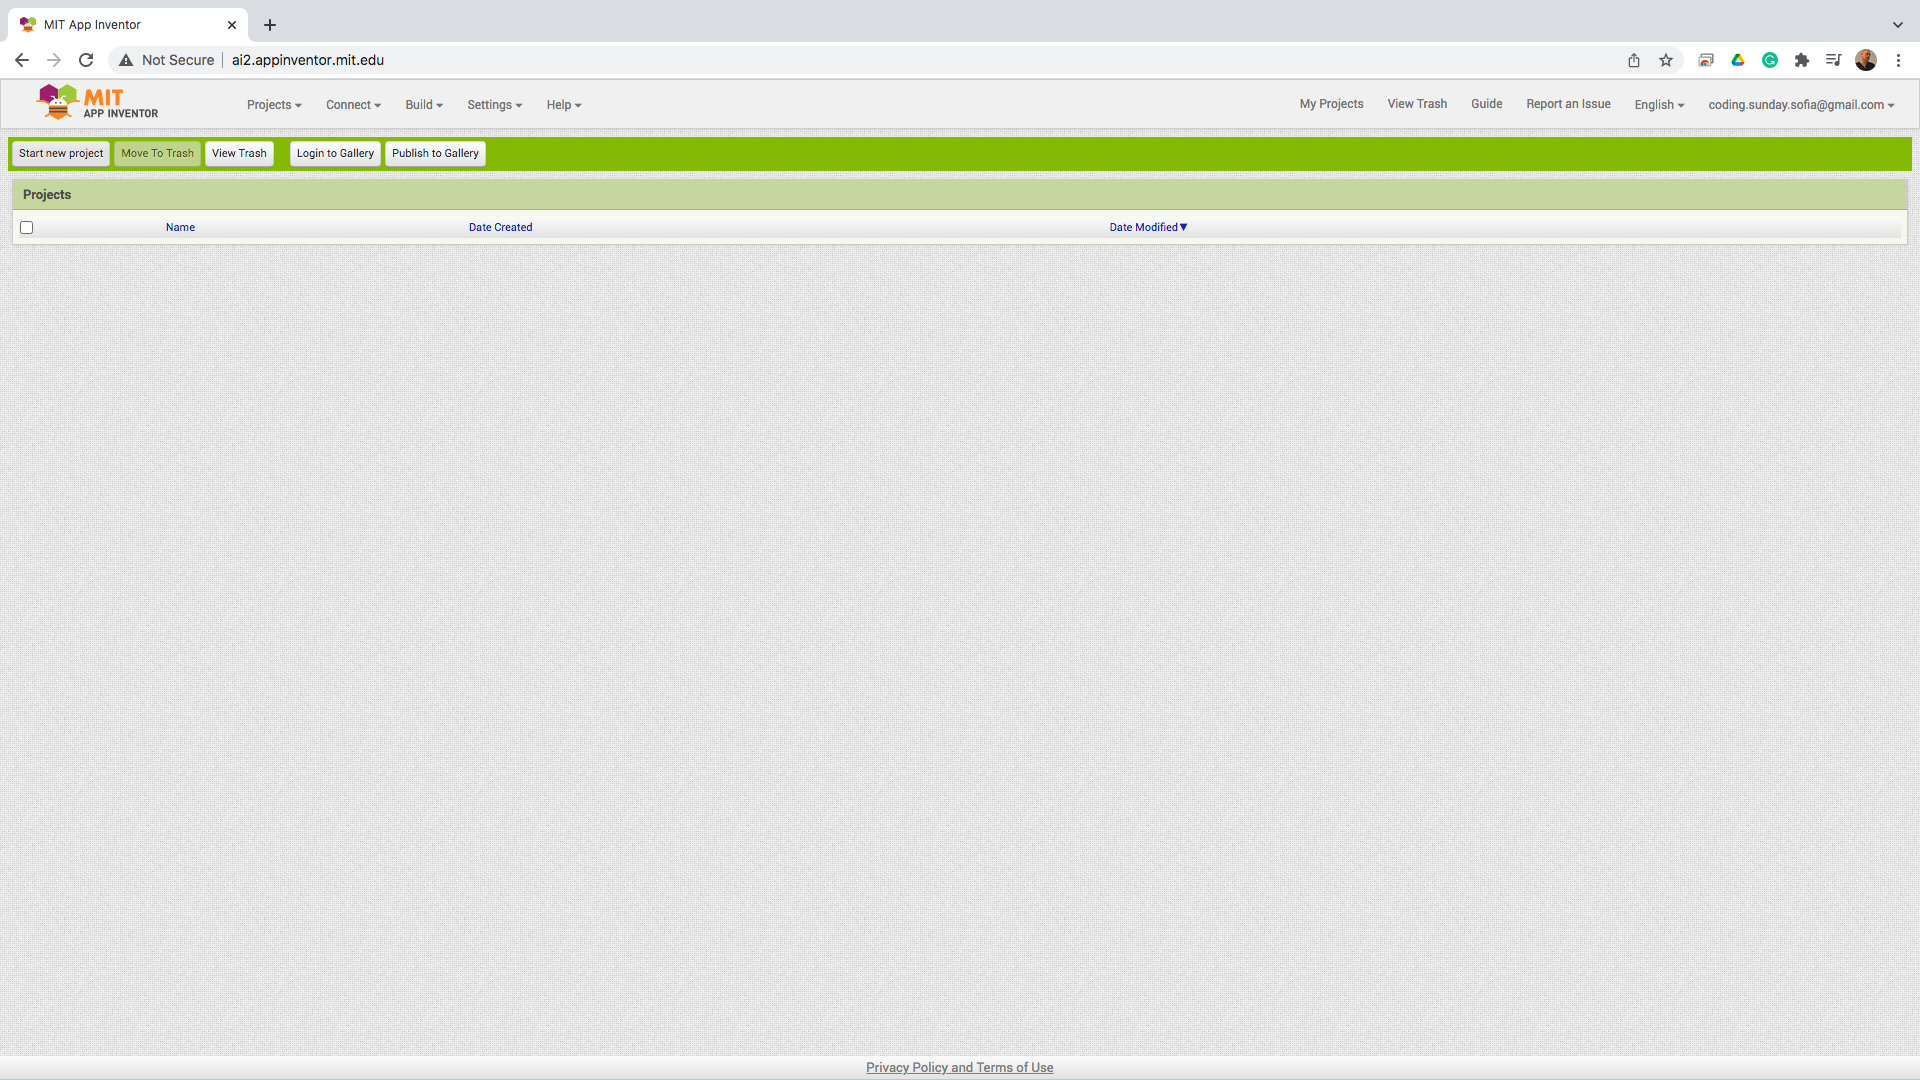
\includegraphics[width=1.0\linewidth,height=0.5\linewidth]{fig010028.png}
  \caption{Бутон за стартиране на нов проект}
\label{fig010028}
\end{figure}

Програмната среда на App Inventor организира работата върху програмен код под формата на проекти. Всеки проект трябва да има подходящо название, което се задава още при създаването на проекта (Фиг. \ref{fig010029}).

\begin{figure}[H]
  \centering
  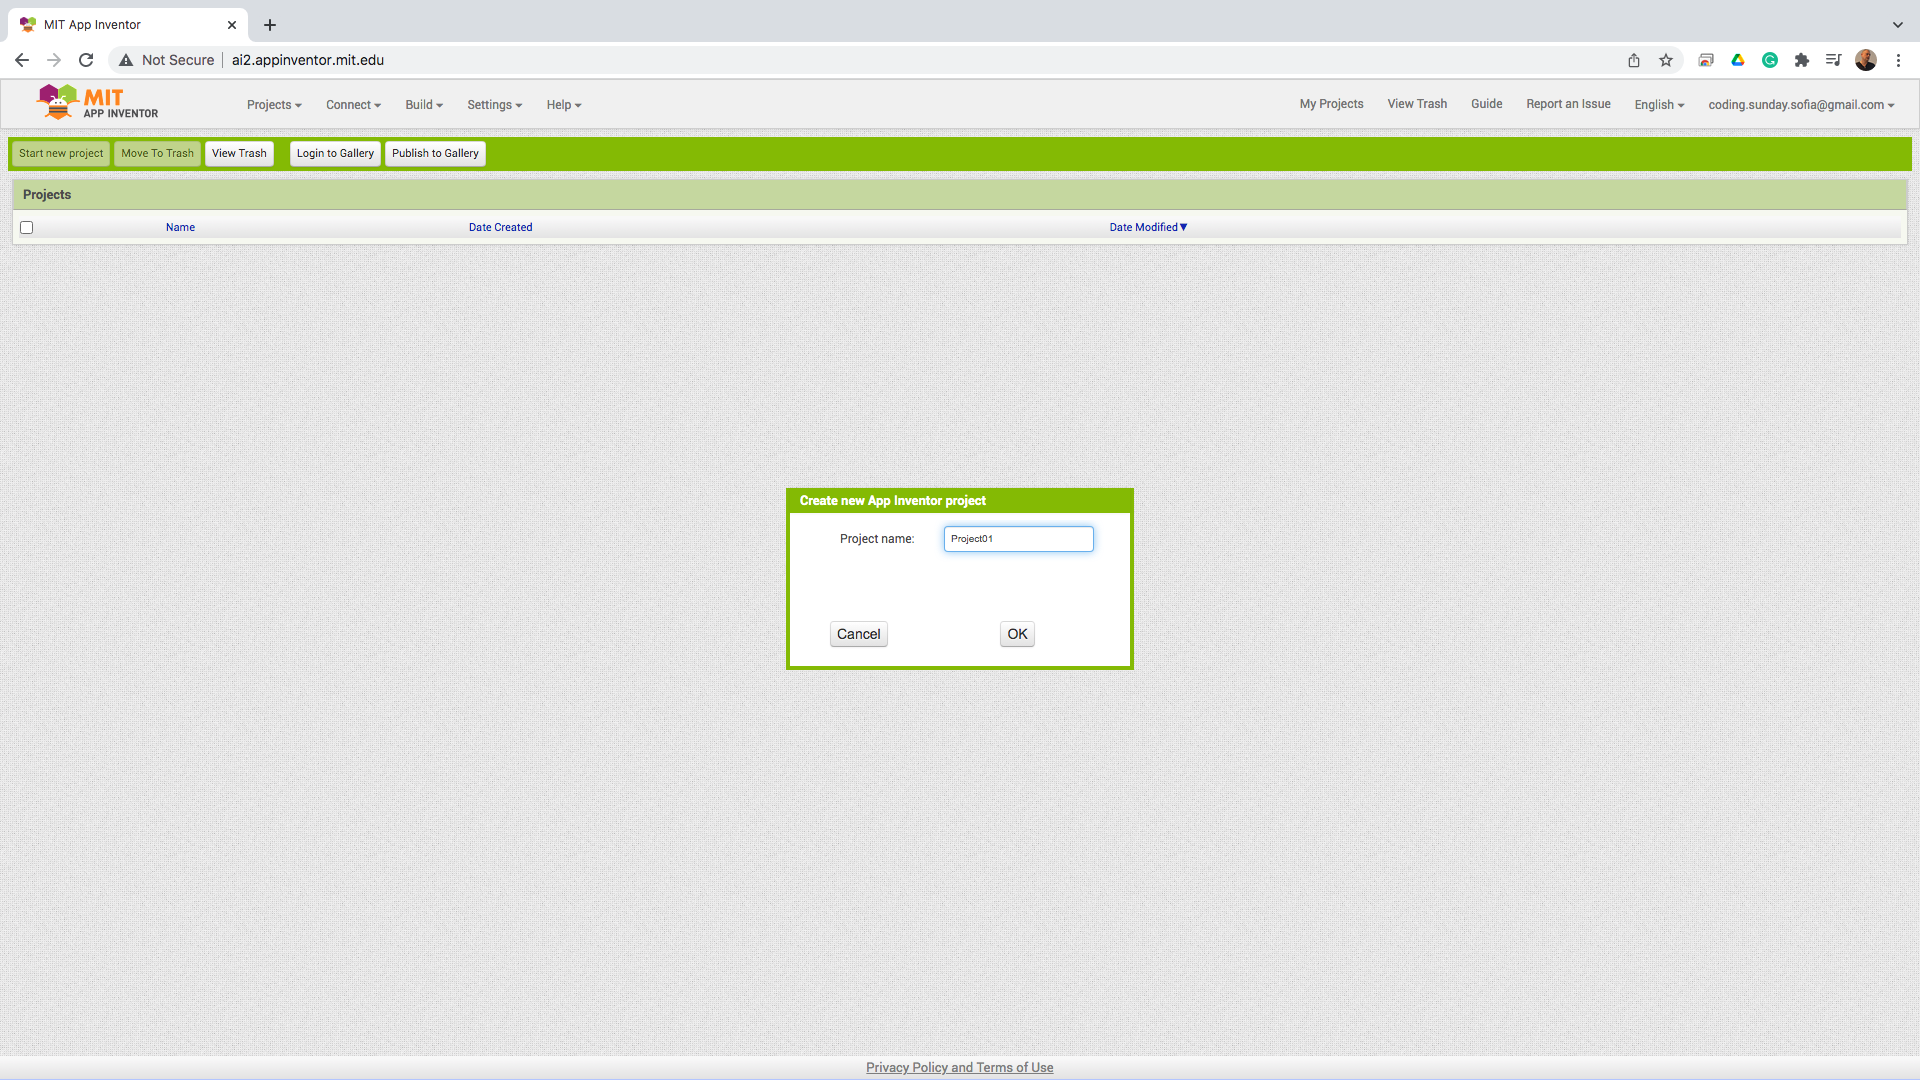
\includegraphics[width=1.0\linewidth,height=0.5\linewidth]{fig010029.png}
  \caption{Название на проекта}
\label{fig010029}
\end{figure}

След избора на название, програмната среда визуализира първият работен екран, даващ възможност за проектиране на визуалния потребителски интерфейс (Фиг. \ref{fig010030}). Проектирането на визуалния потребителски интерфейс се случва, чрез придърпване на различните визуални контроли в основната работна площ. 

\begin{figure}[H]
  \centering
  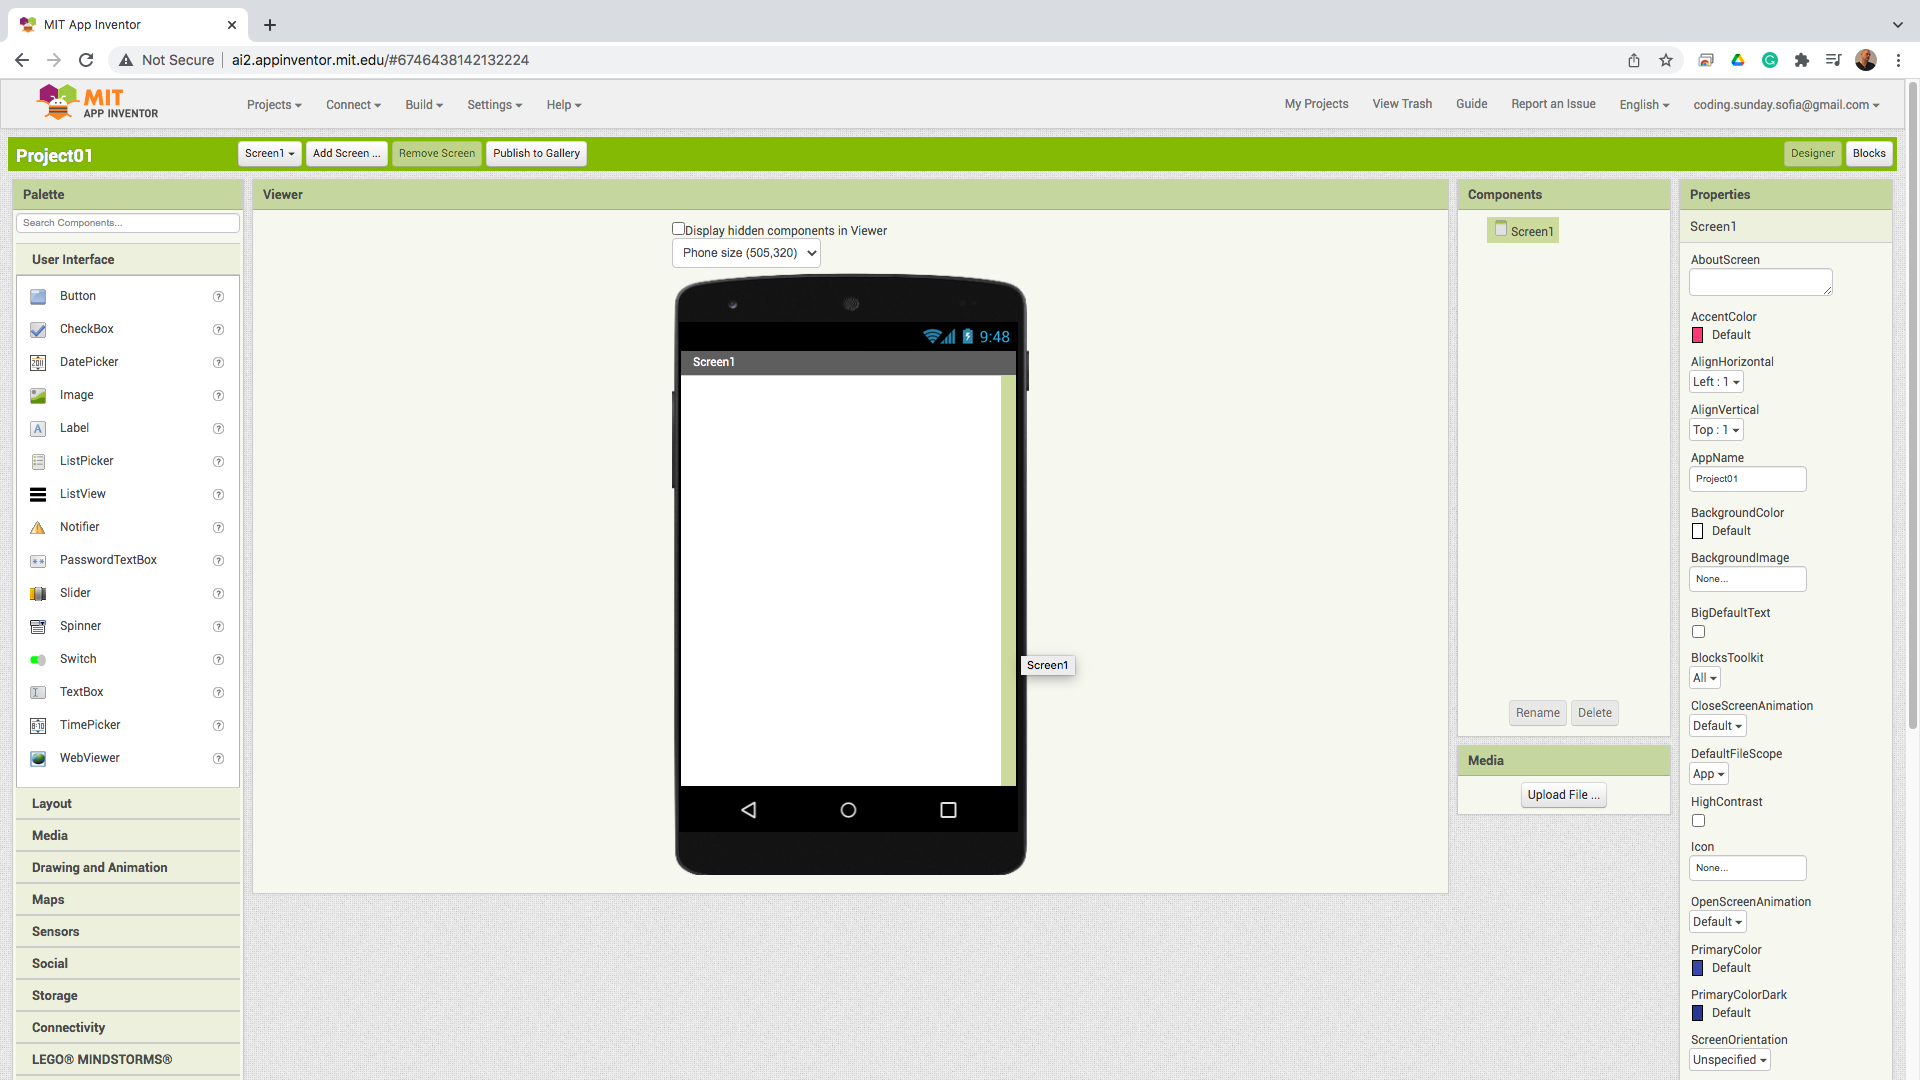
\includegraphics[width=1.0\linewidth,height=0.5\linewidth]{fig010030.png}
  \caption{Проектантски изглед на развойната среда}
\label{fig010030}
\end{figure}

Един от най-базовите визуални контроли е бутонът. Представлява обособена зона във визуалното поле, която има текстово надписване или икона за визуално представяне на действието, извършвано след натискането на бутона. За демонстрирането на процеса по работа със съставения програмен код се използва един бутон (Фиг. \ref{fig010031}).

\begin{figure}[H]
  \centering
  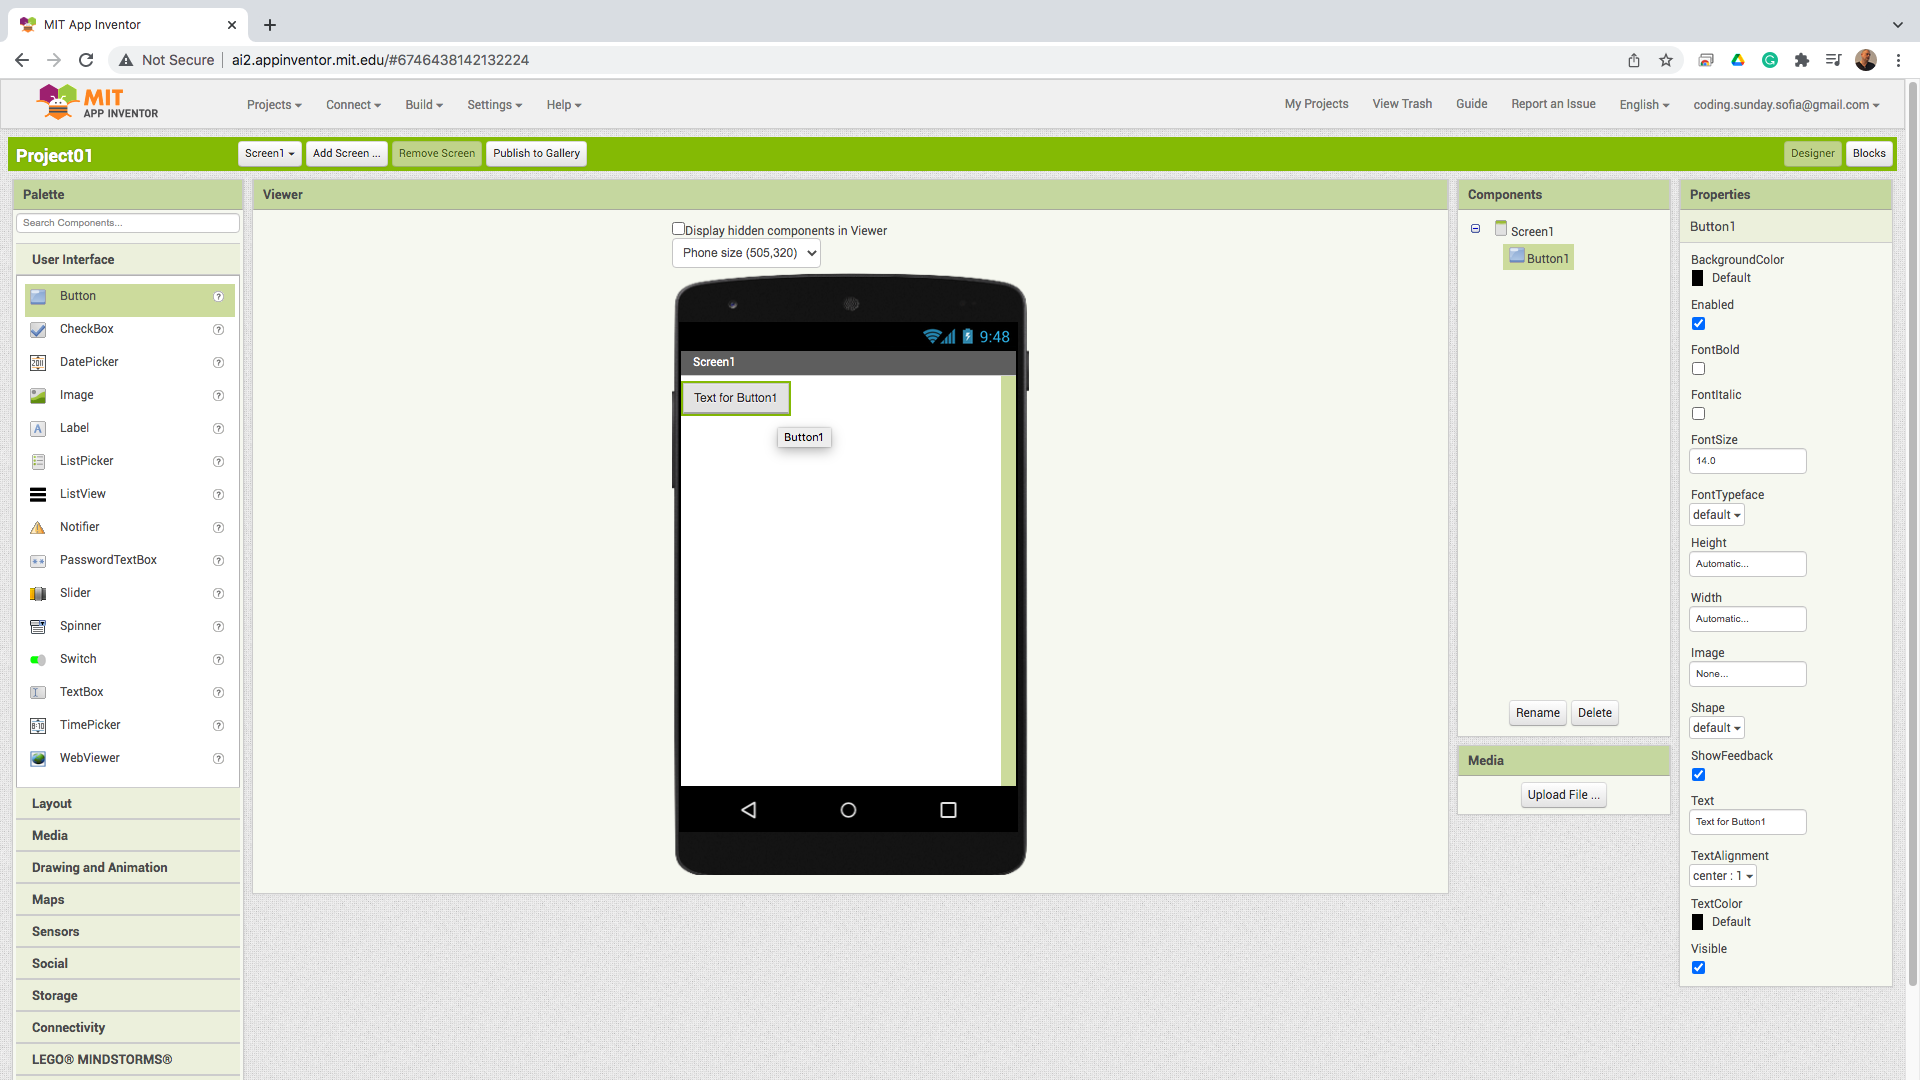
\includegraphics[width=1.0\linewidth,height=0.5\linewidth]{fig010031.png}
  \caption{Поставяне на бутон}
\label{fig010031}
\end{figure}

От съществено значение е за хората използващи софтуерното приложение, бутоните да имат максимално експресивни названия. В случая, целта е бутонът да бъде натиснат и от това да последва конкретно действие. Поради тази причина, названието на бутона е само „Push“ (Фиг. \ref{fig010031}).

\begin{figure}[H]
  \centering
  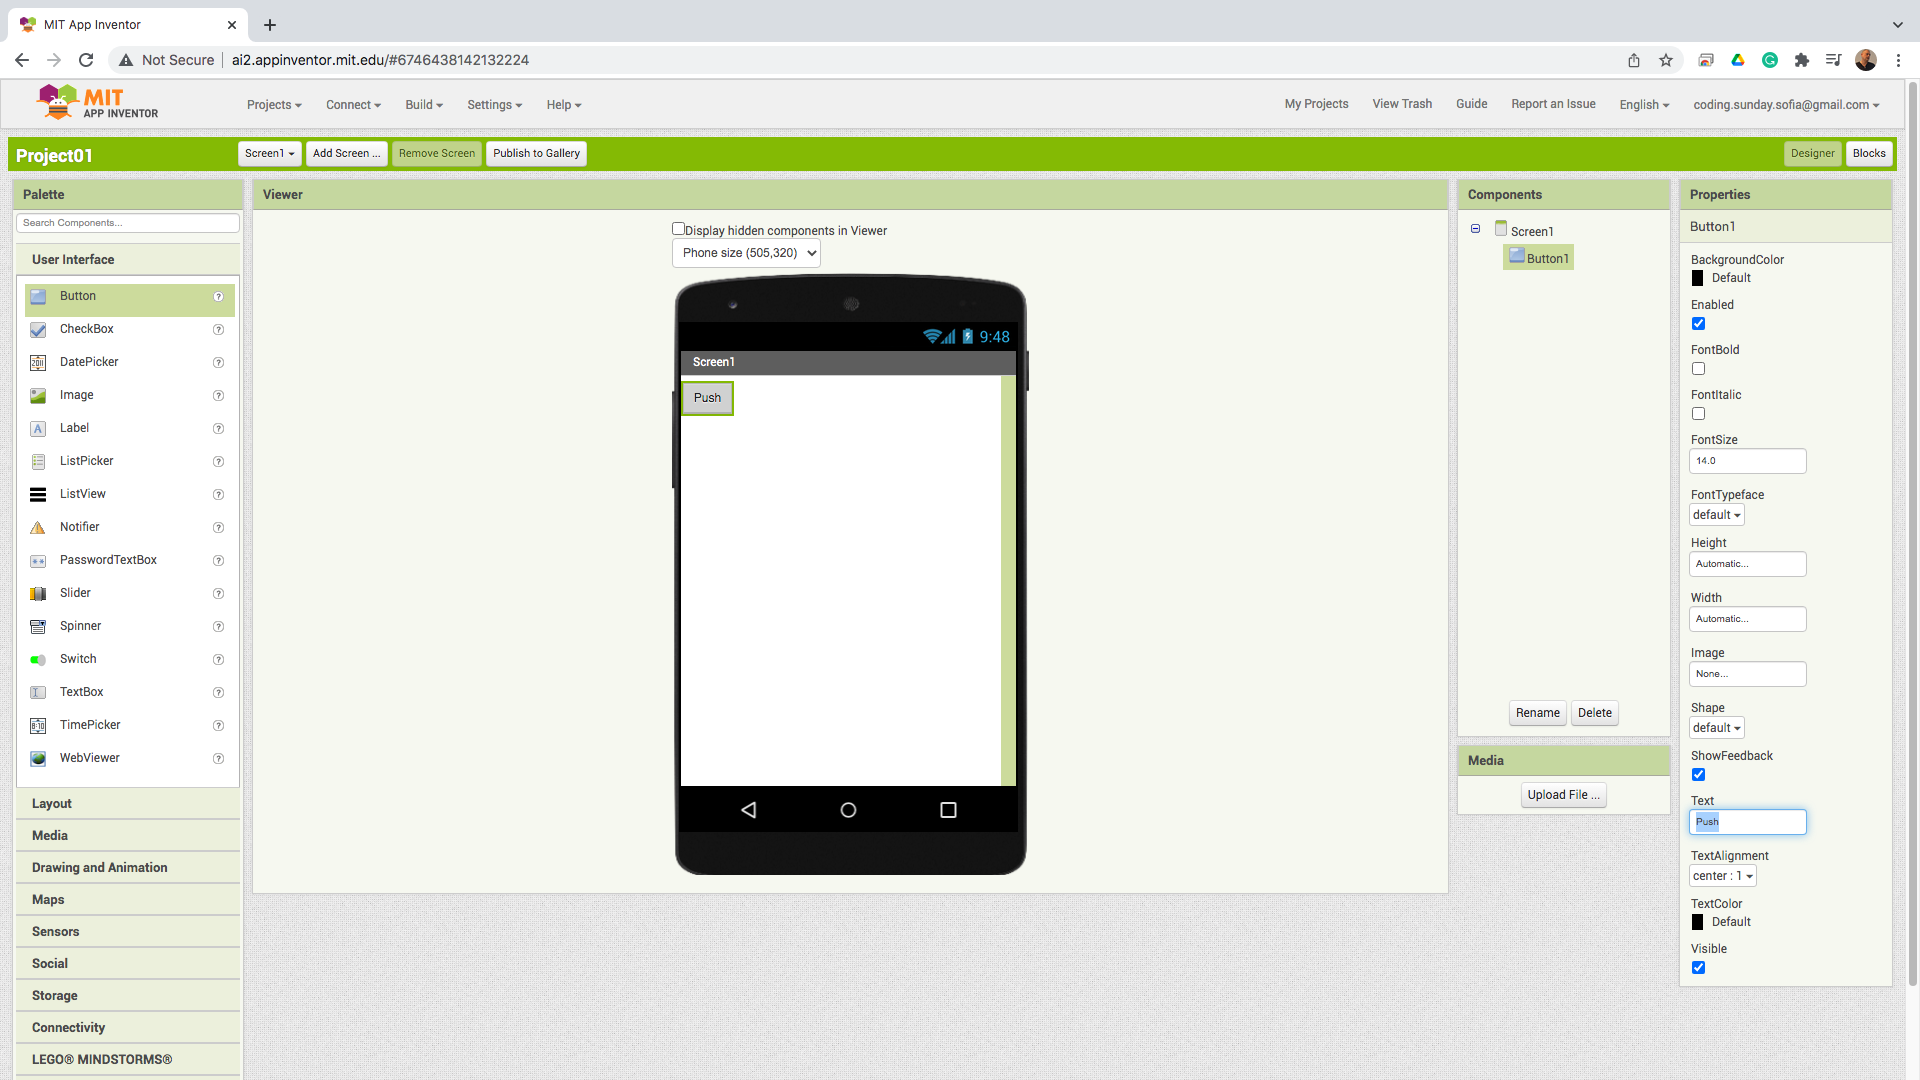
\includegraphics[width=1.0\linewidth,height=0.5\linewidth]{fig010032.png}
  \caption{Избор на текст върху бутона}
\label{fig010032}
\end{figure}

За разлика от програмната среда Scratch, при App Inventor програмните инструкции се подрежат под формата на пъзел в отделен работен екран (Фиг. \ref{fig010033}). 

\begin{figure}[H]
  \centering
  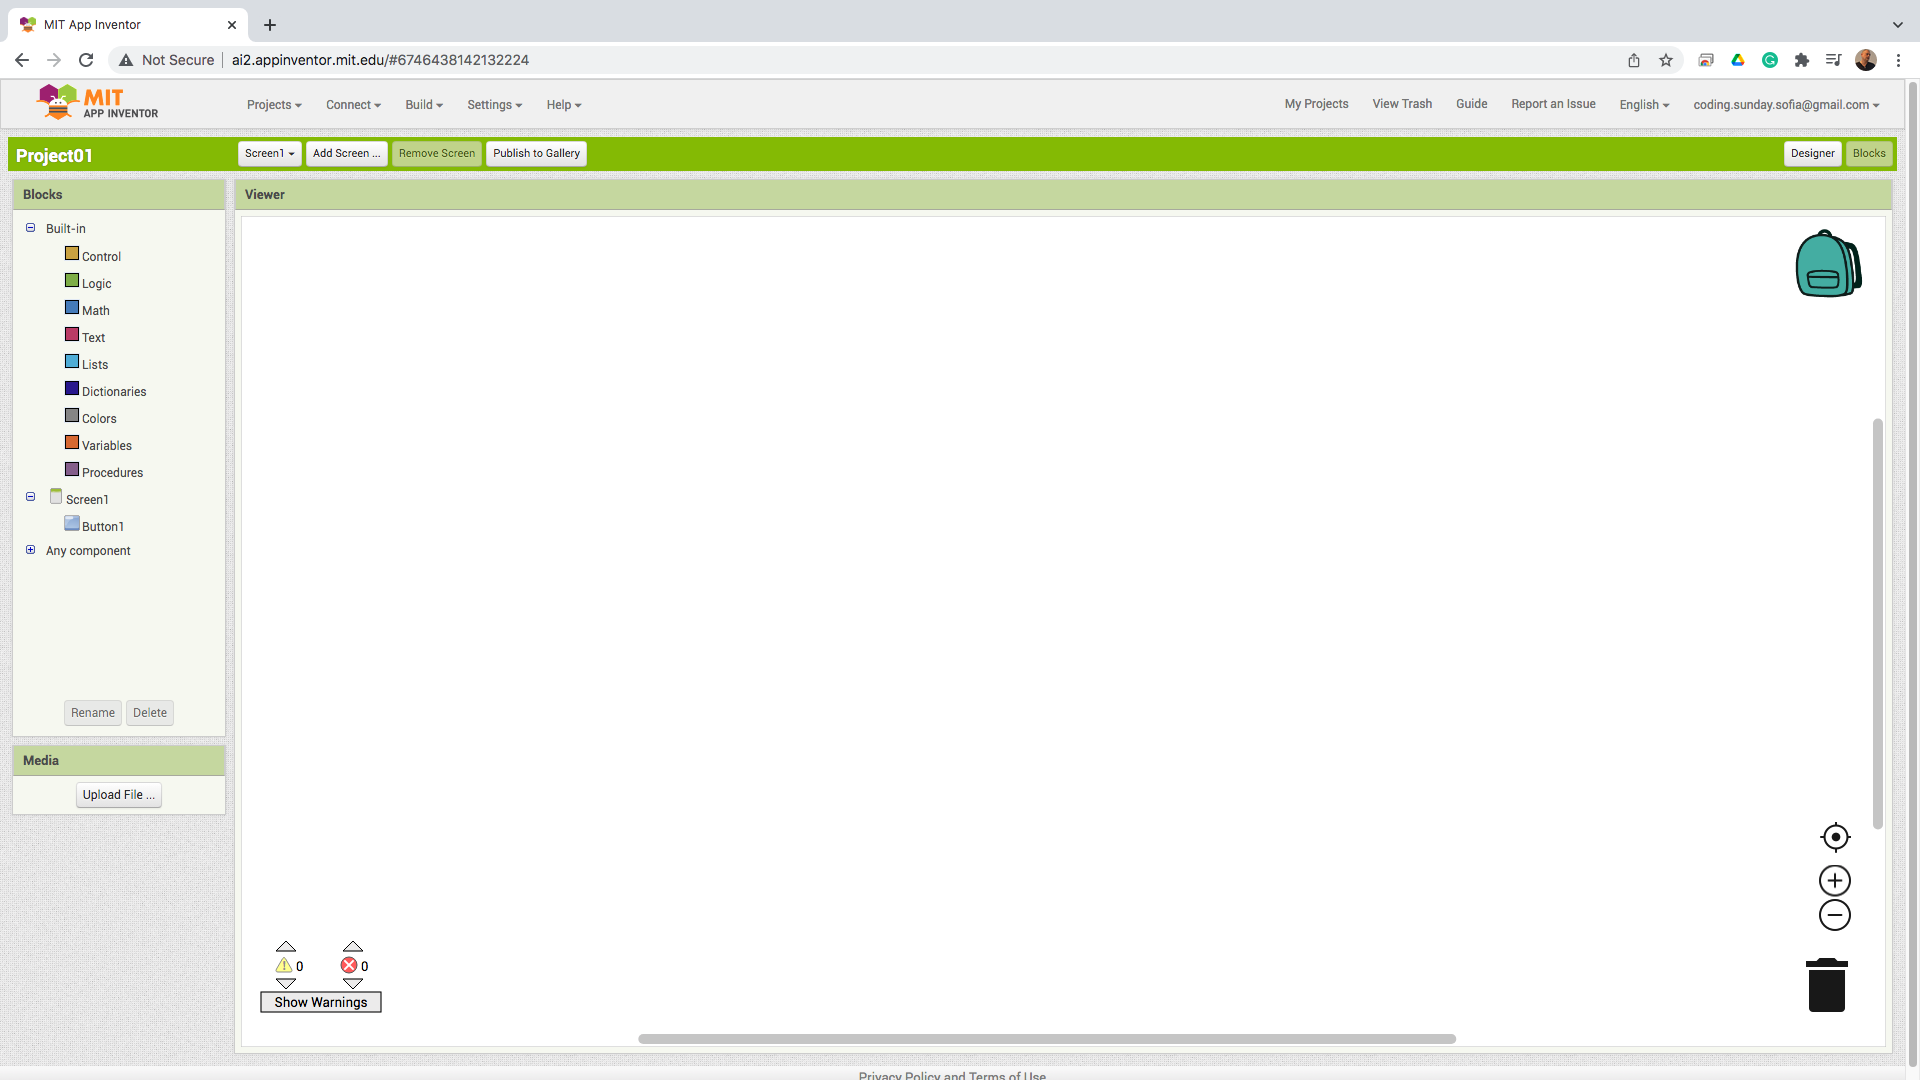
\includegraphics[width=1.0\linewidth,height=0.5\linewidth]{fig010033.png}
  \caption{Програмен изглед на развойната среда}
\label{fig010033}
\end{figure}

Тъй като графичният потребителски интерфейс до момента се състои само от единствен компонент (бутон), то някакви инструкции могат да се изпълнят единствено с този визуален компонент. За разлика от Scratch, където програмата има начална стартова точка и финална крайна точка, при App Inventor програмните инструкции се подреждат на принципа на възникващите събития. Когато програмата започне да работи, тя визуализира графичния потребителски интерфейс и очаква от ползващия устройството да извърши някакво действие (Фиг. \ref{fig010034}). 

\begin{figure}[H]
  \centering
  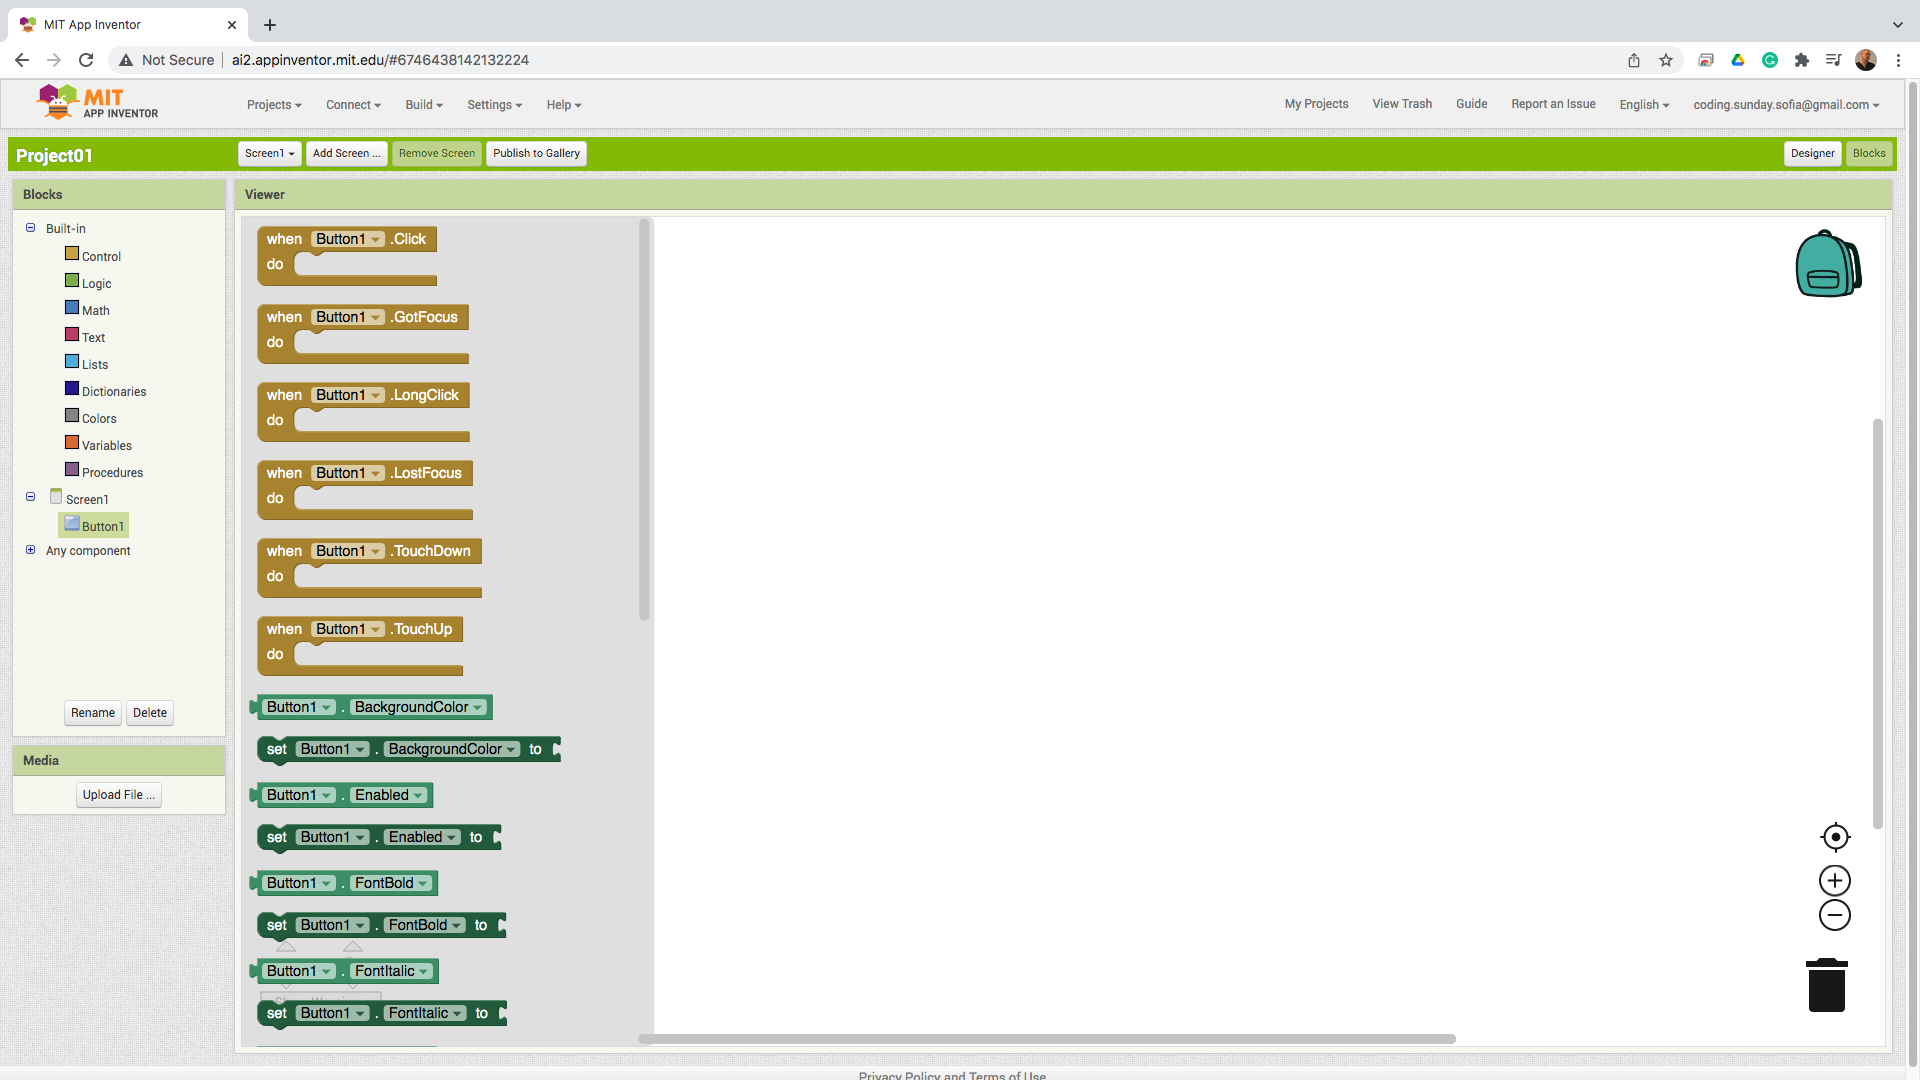
\includegraphics[width=1.0\linewidth,height=0.5\linewidth]{fig010034.png}
  \caption{Списък с инструкции}
\label{fig010034}
\end{figure}

Такова действие би могло да бъде натискането на бутон. От страната на App Inventor, натиснатият бутон генерира събитие (event), за което събитие се избират конкретни действия на програмата (Фиг. \ref{fig010035}). 

\begin{figure}[H]
  \centering
  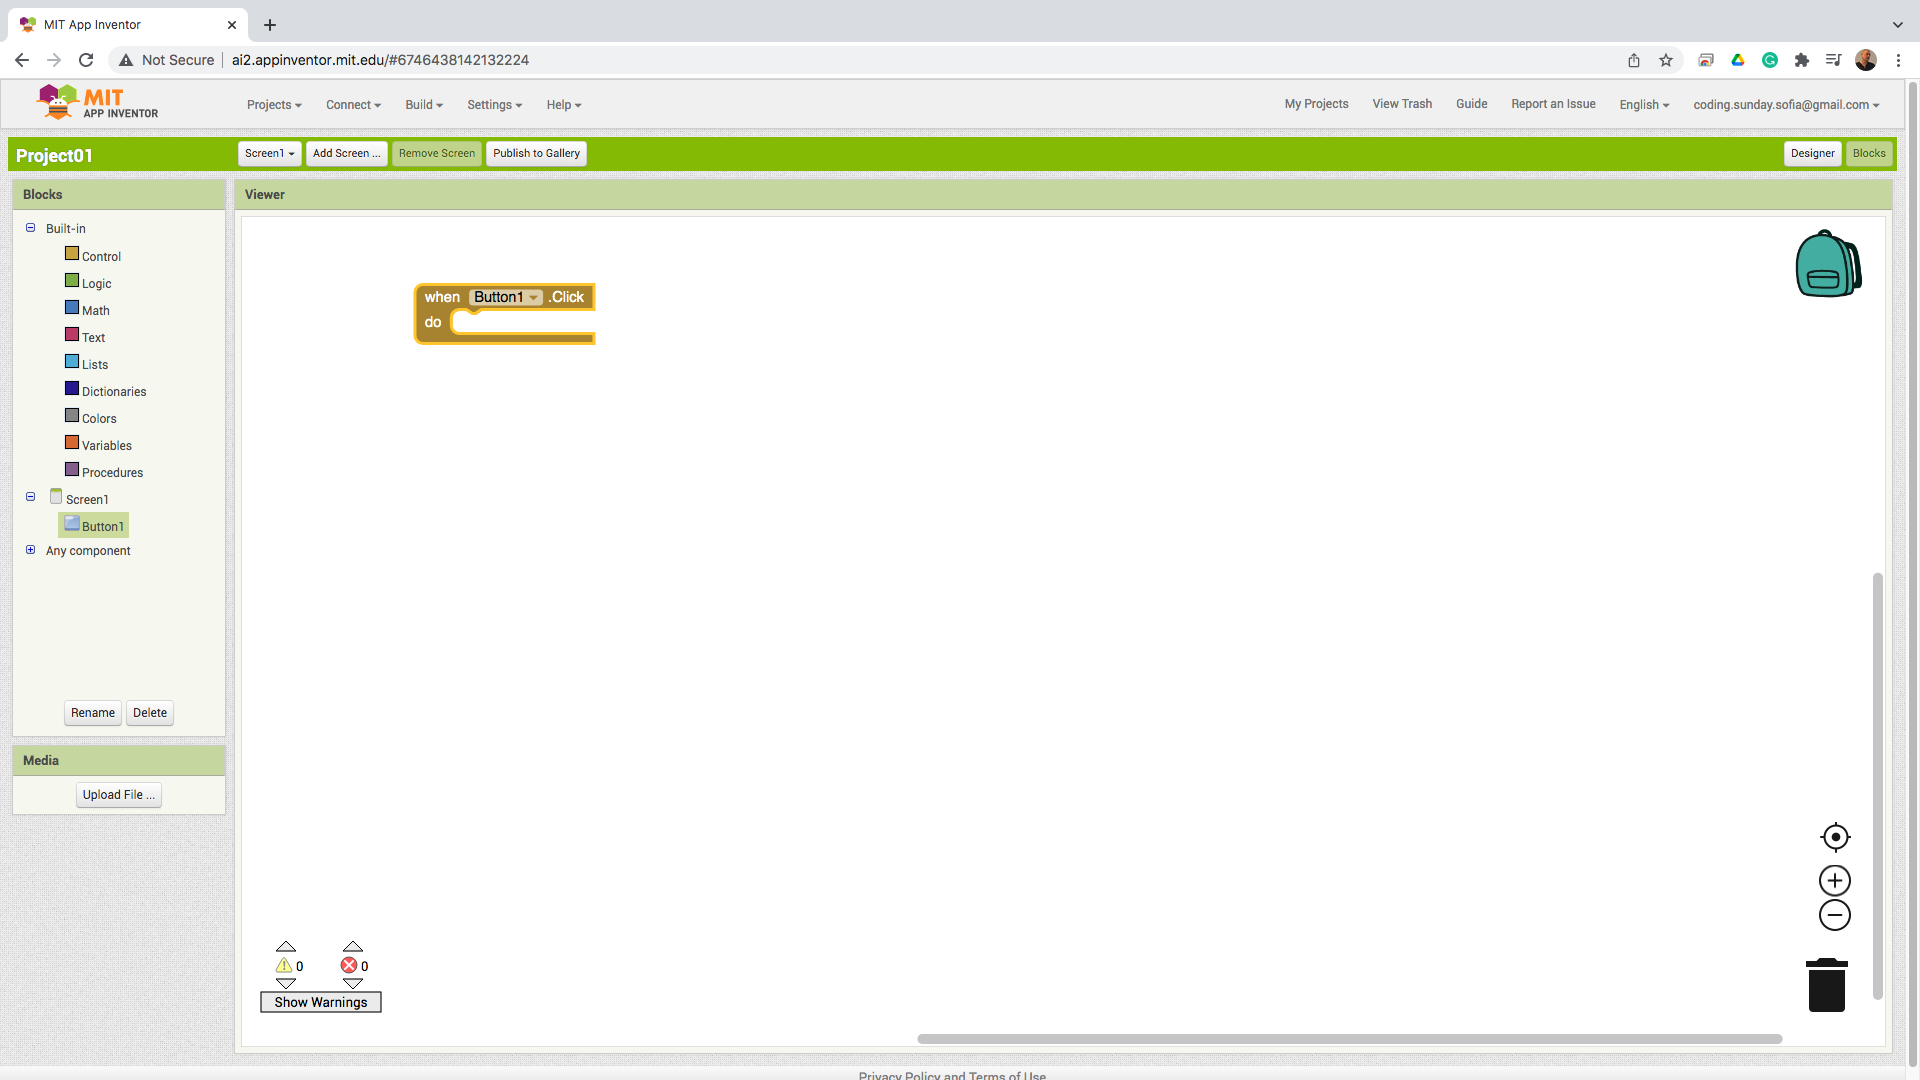
\includegraphics[width=1.0\linewidth,height=0.5\linewidth]{fig010035.png}
  \caption{Избор на събитие за натискане на бутона}
\label{fig010035}
\end{figure}

Събитието за натискане на бутон се визуализира под формата на парче от пъзел, съдържащо слот в който могат да се подредят инструкциите, които трябва да се изпълнят (Фиг. \ref{fig010036}).

\begin{figure}[H]
  \centering
  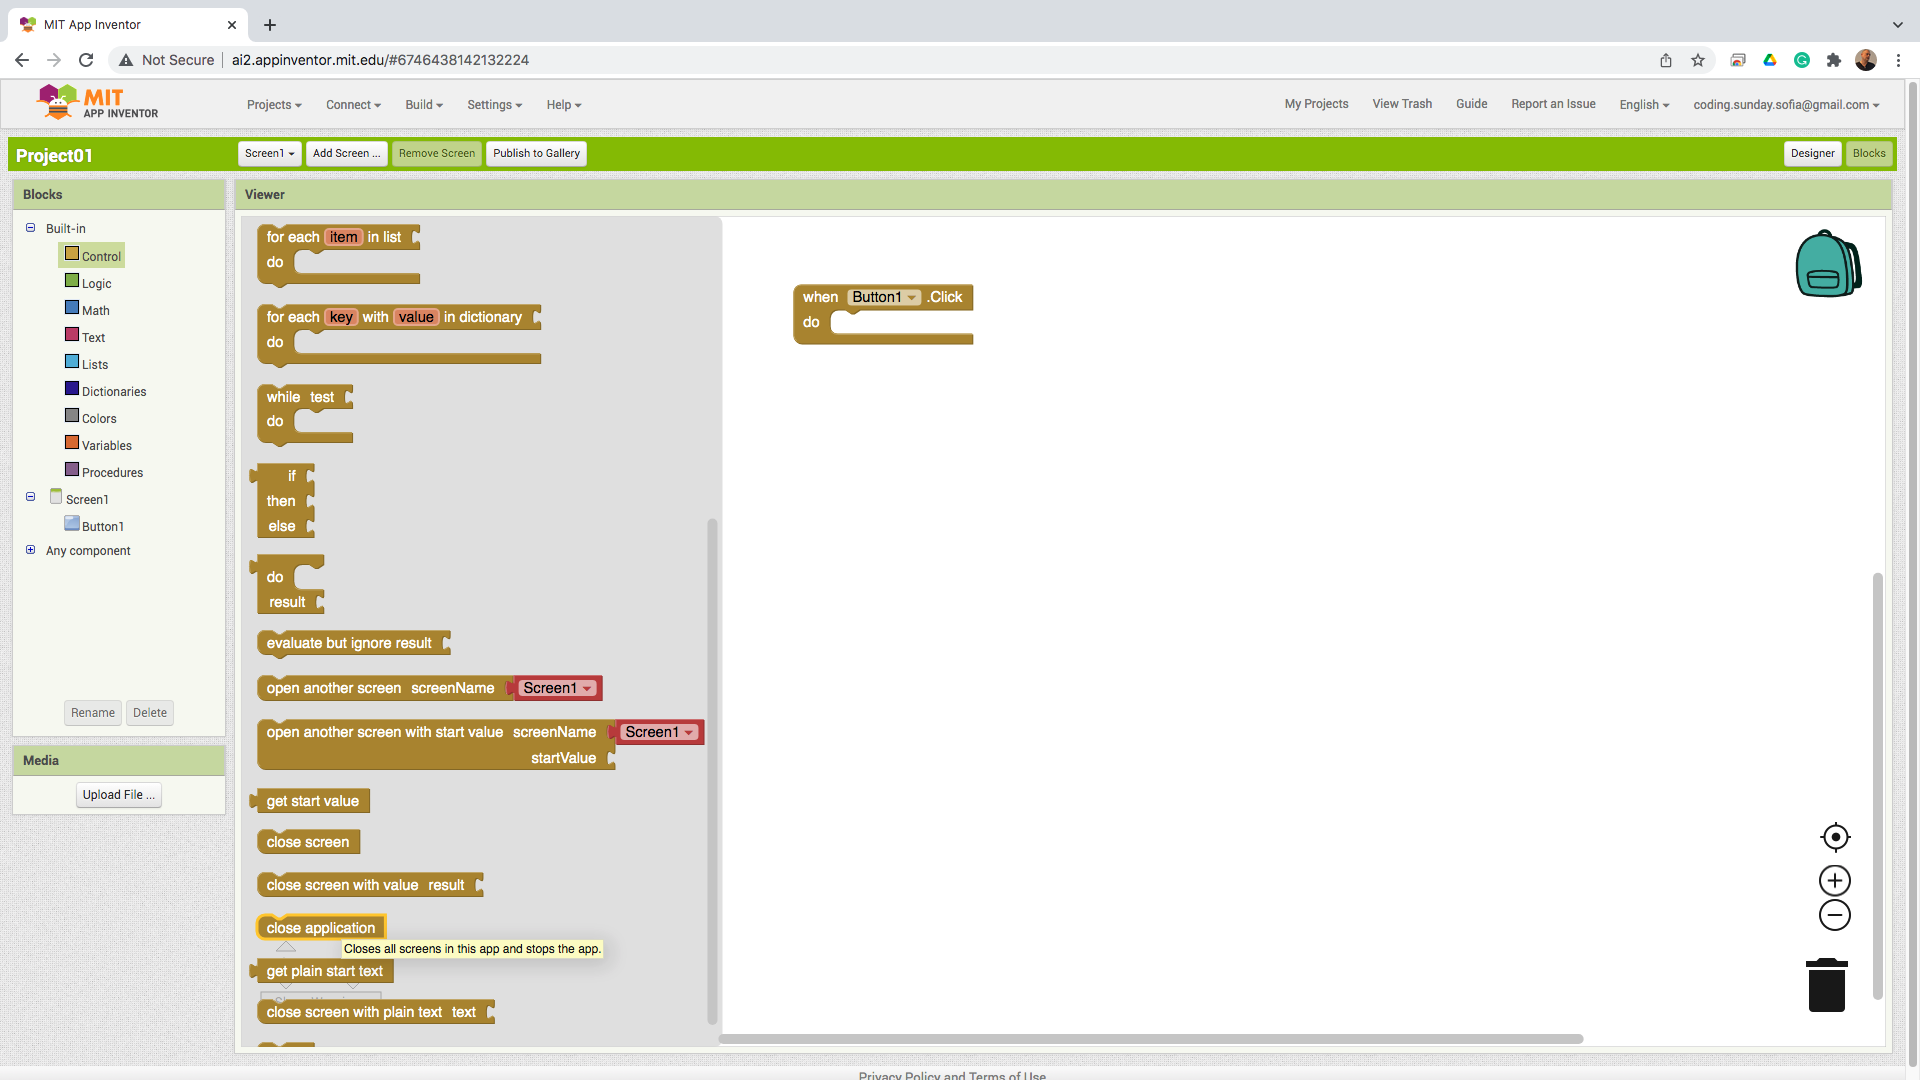
\includegraphics[width=1.0\linewidth,height=0.5\linewidth]{fig010036.png}
  \caption{Избор на действие при натискане на бутона}
\label{fig010036}
\end{figure}

Най-простичкото действие, което може да бъде изпълнено, след натискането на бутона е програмата да бъде спряна и прозорецът на разработваното приложение да бъде затворен (Фиг. \ref{fig010037}).

\begin{figure}[H]
  \centering
  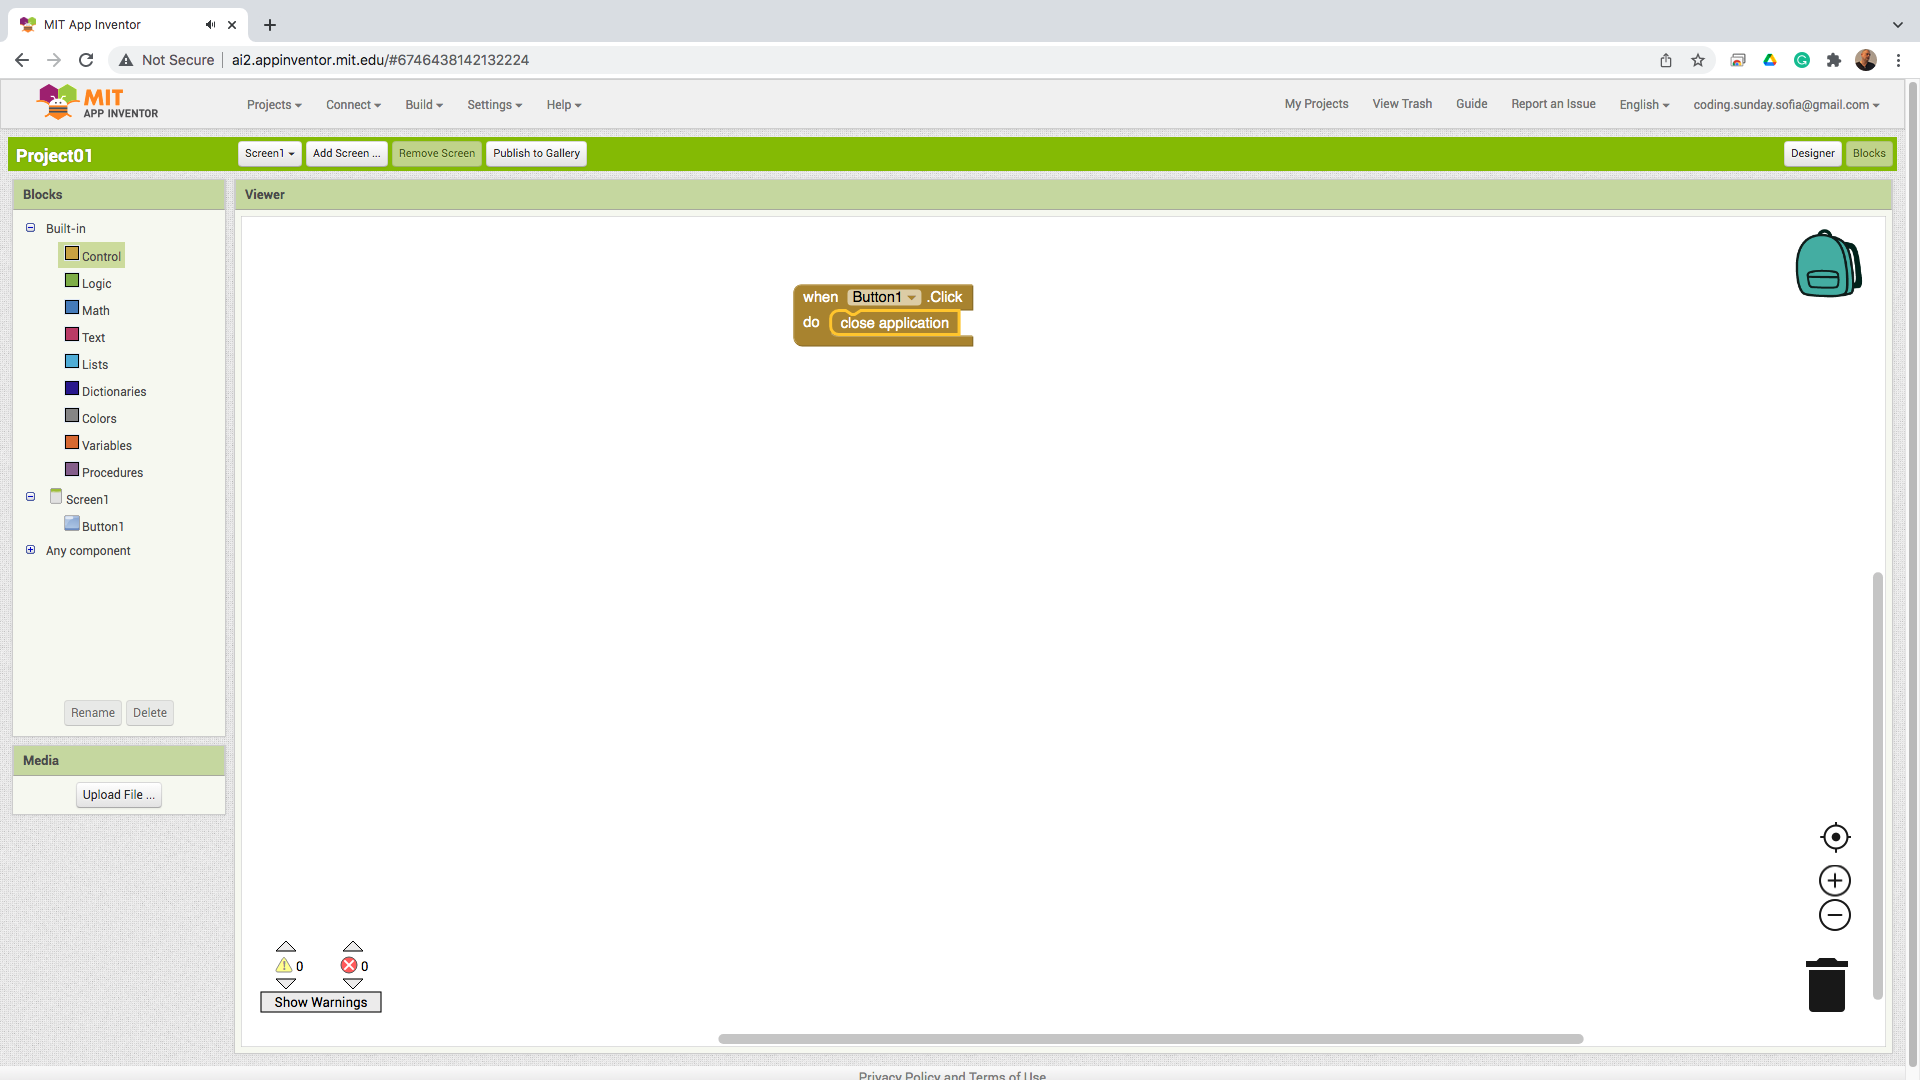
\includegraphics[width=1.0\linewidth,height=0.5\linewidth]{fig010037.png}
  \caption{Затваряне на приложението при натискане на бутона}
\label{fig010037}
\end{figure}

След като графичният програмен интерфейс е оформен и желаните за изпълнение инструкции са подредени, следва компилирането на кода и изграждането на цялостния инсталационен пакет за написаната програма (Фиг. \ref{fig010038}). 

\begin{figure}[H]
  \centering
  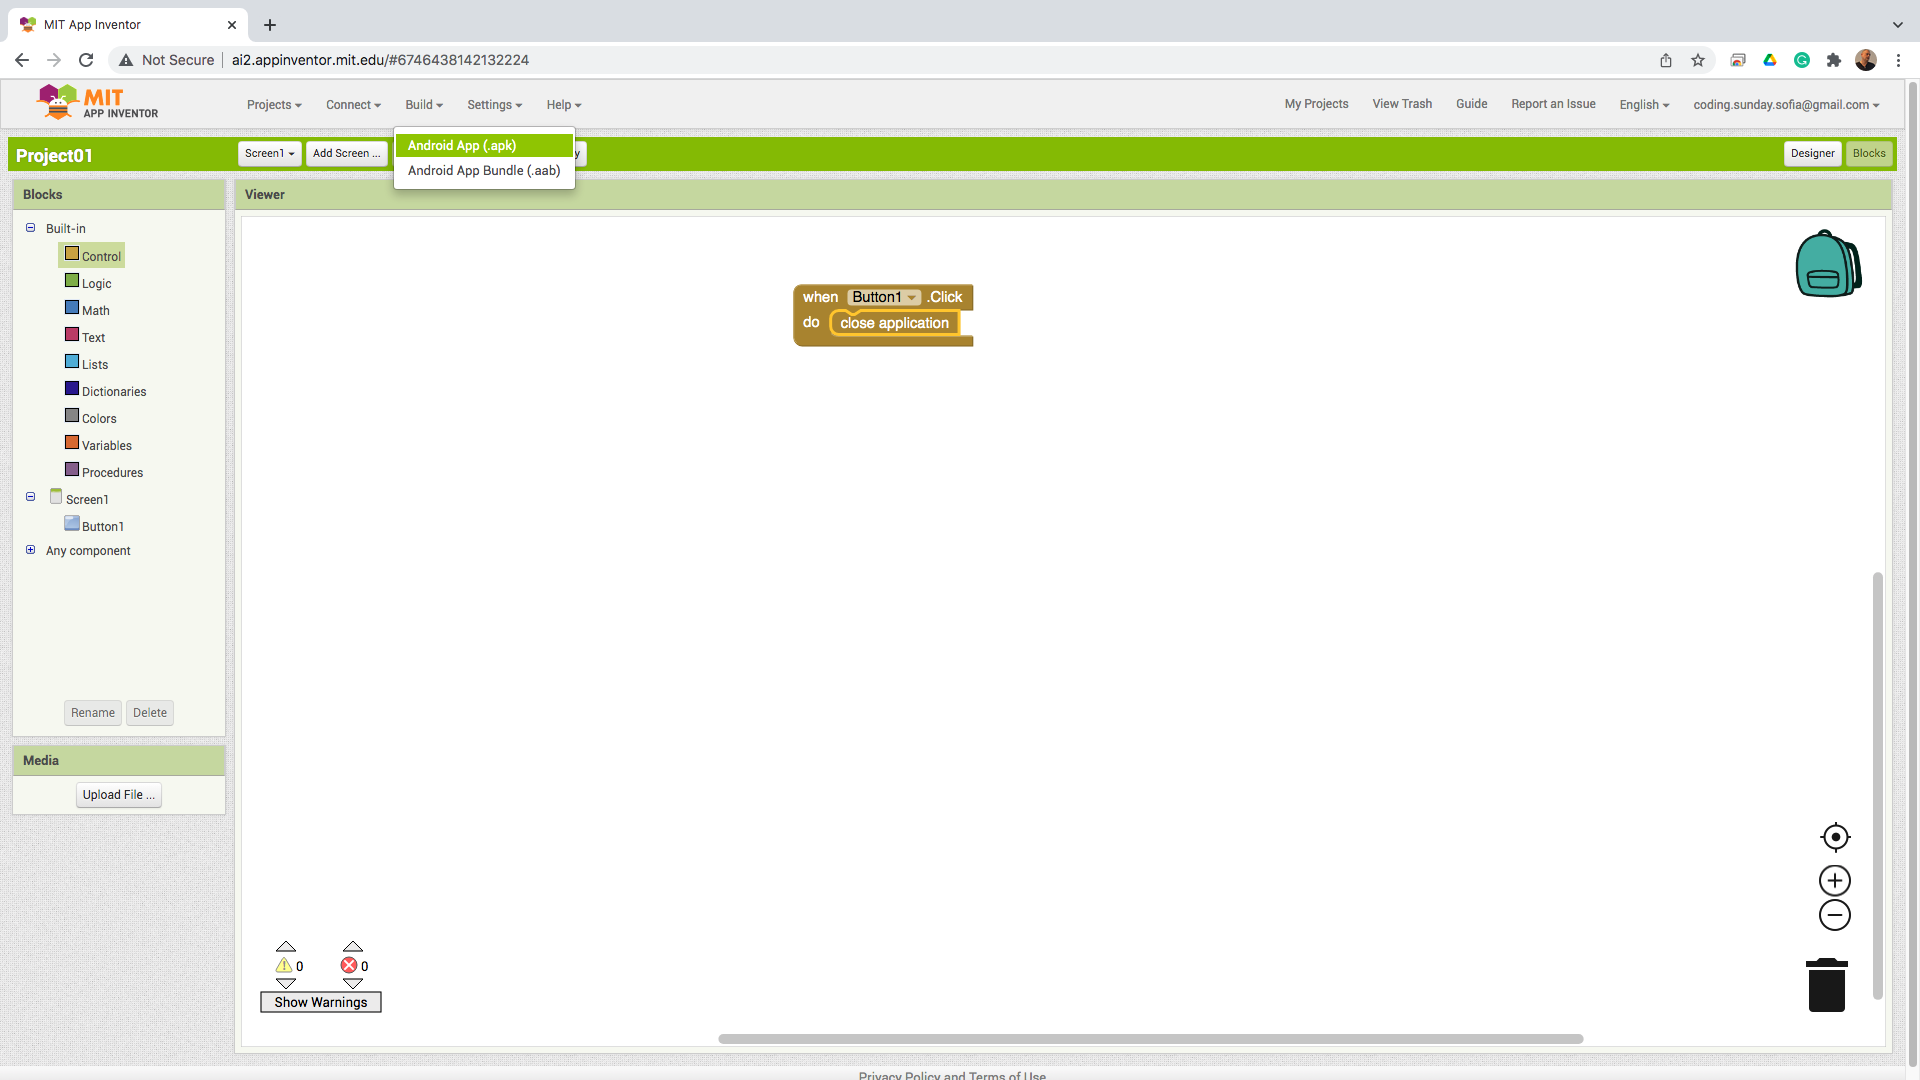
\includegraphics[width=1.0\linewidth,height=0.5\linewidth]{fig010038.png}
  \caption{Меню за изграждане на мобилното приложение}
\label{fig010038}
\end{figure}

Фундаментална разлика между Scratch и App Inventor е, че резултатът от изпълнението на програмните инструкции при Scratch се виждат в самото работно пространство на програмната среда, докато при App Inventor инсталационния пакет на програмата бива компилиран в облачната структура, след това трябва да се изтегли и инсталира на мобилно устройство. Процесът по компилация и изграждане на инсталационния пакет изисква определено изчислително време, визуализирано под формата на прогрес бар (Фиг. \ref{fig010039}).

\begin{figure}[H]
  \centering
  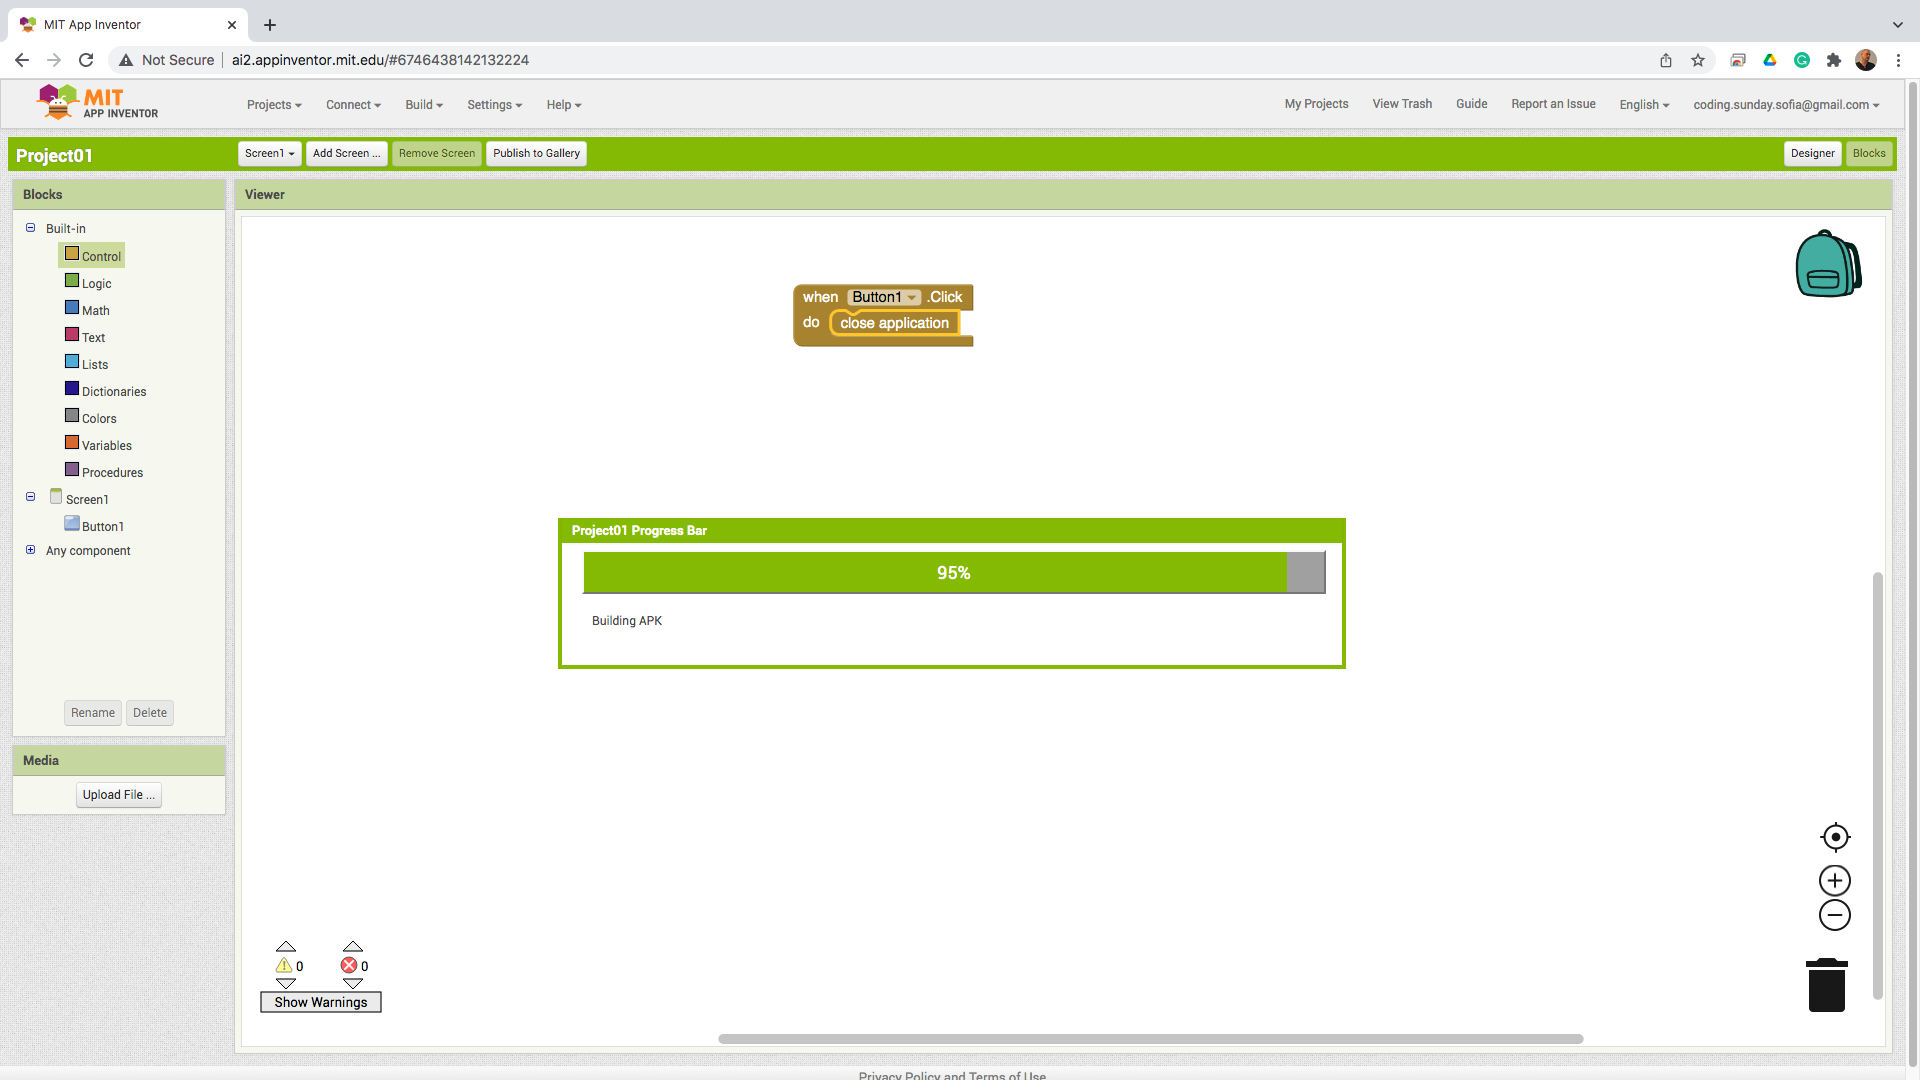
\includegraphics[width=1.0\linewidth,height=0.5\linewidth]{fig010039.png}
  \caption{Прогрес при изграждането на приложението}
\label{fig010039}
\end{figure}

След като проектът е компилиран и инсталационният пакет е създаден, програмната среда предлага QR код (Фиг. \ref{fig010040}), чрез който инсталационния пакет да бъде изтеглен от мобилното устройство (телефон или таблет).

\begin{figure}[H]
  \centering
  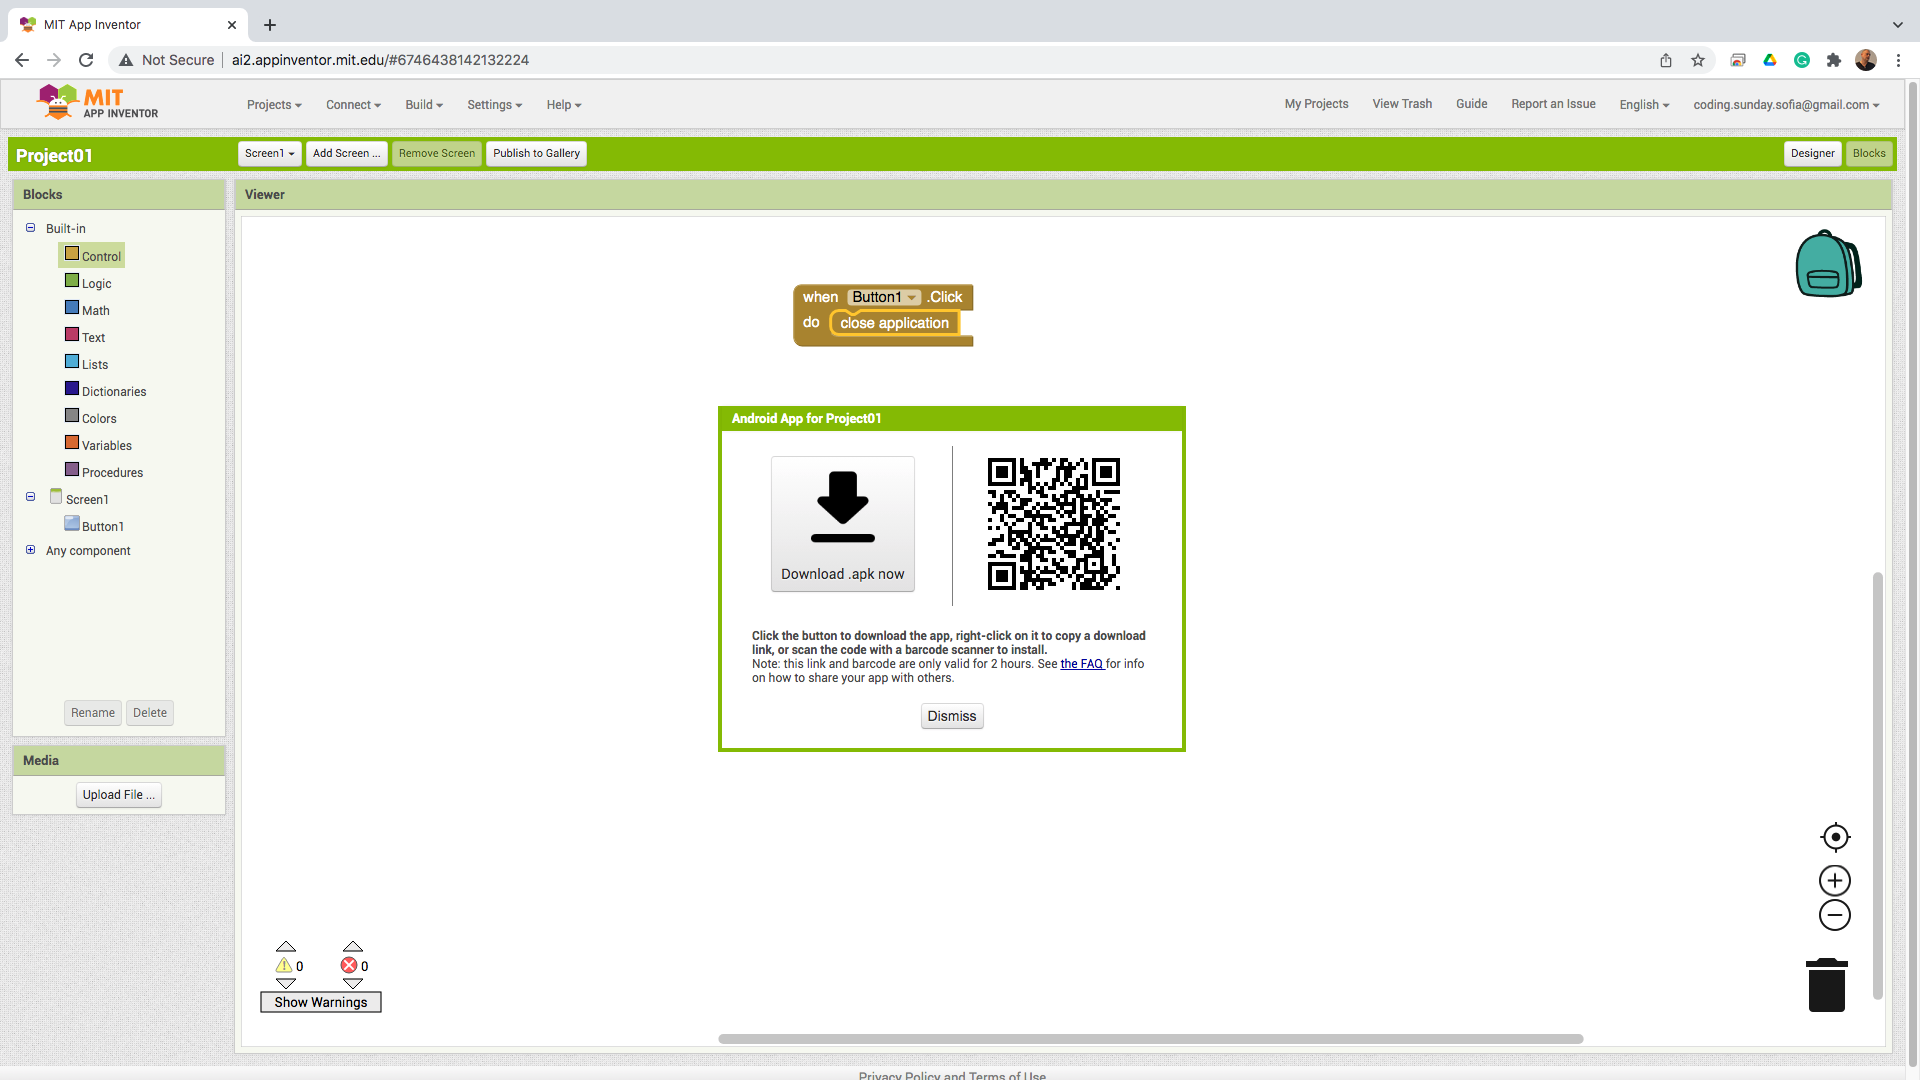
\includegraphics[width=1.0\linewidth,height=0.5\linewidth]{fig010040.png}
  \caption{Код за инсталация на приложението върху мобилно устройство}
\label{fig010040}
\end{figure}

Създателите на програмната среда App Inventor са предвидили възможност за по-бърза и лесна инсталация на написаните програми, чрез специално създадено приложение (MIT AI2 Companion), което да поеме комуникацията с облачната инфраструктура на App Inventor (Фиг. \ref{fig010041}). Приложението е достъпно в Google Play и не изисква никакви специални умения за да бъде инсталирано на личното мобилно устройство. 

\begin{figure}[H]
  \centering
  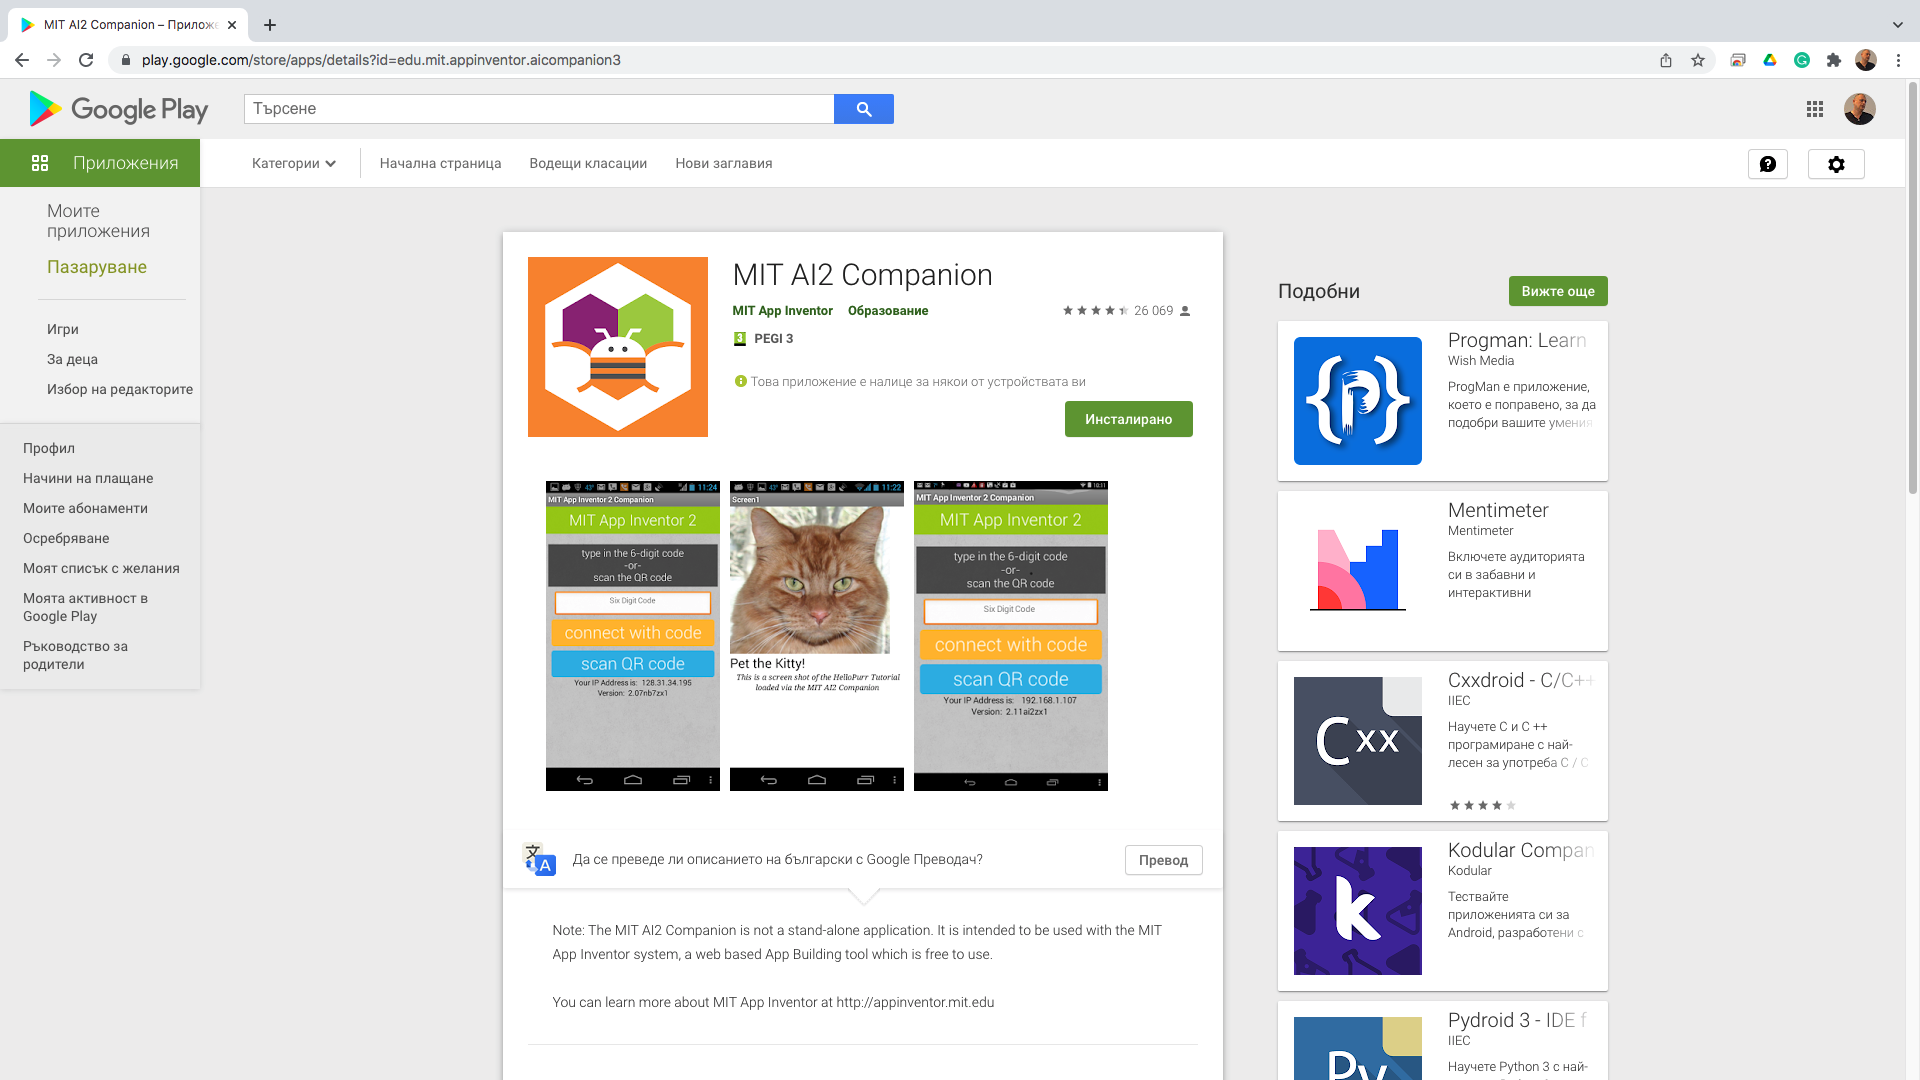
\includegraphics[width=1.0\linewidth,height=0.5\linewidth]{fig010041.png}
  \caption{Мобилно приложение за управление на компилираните проекти}
\label{fig010041}
\end{figure}

Когато се стартира MIT AI2 Companion, приложението дава две възможности за изтегляне на вече написаните програми (Фиг. \ref{fig010042}). Единият вариант е чрез въвеждане на код, а вторият вариант е чрез сканиране на QR код. Сканирането на QR кода е значително по-бързо и по удобно (Фиг. \ref{fig010043}). Тъй като инсталационният пакет представлява изпълним файл, Android операционната система издава предупреждение, че такива файлове могат да бъдат опасни при използването им (Фиг. \ref{fig010044}).

\begin{figure}[H]
  \begin{subfigure}{0.31\textwidth}
  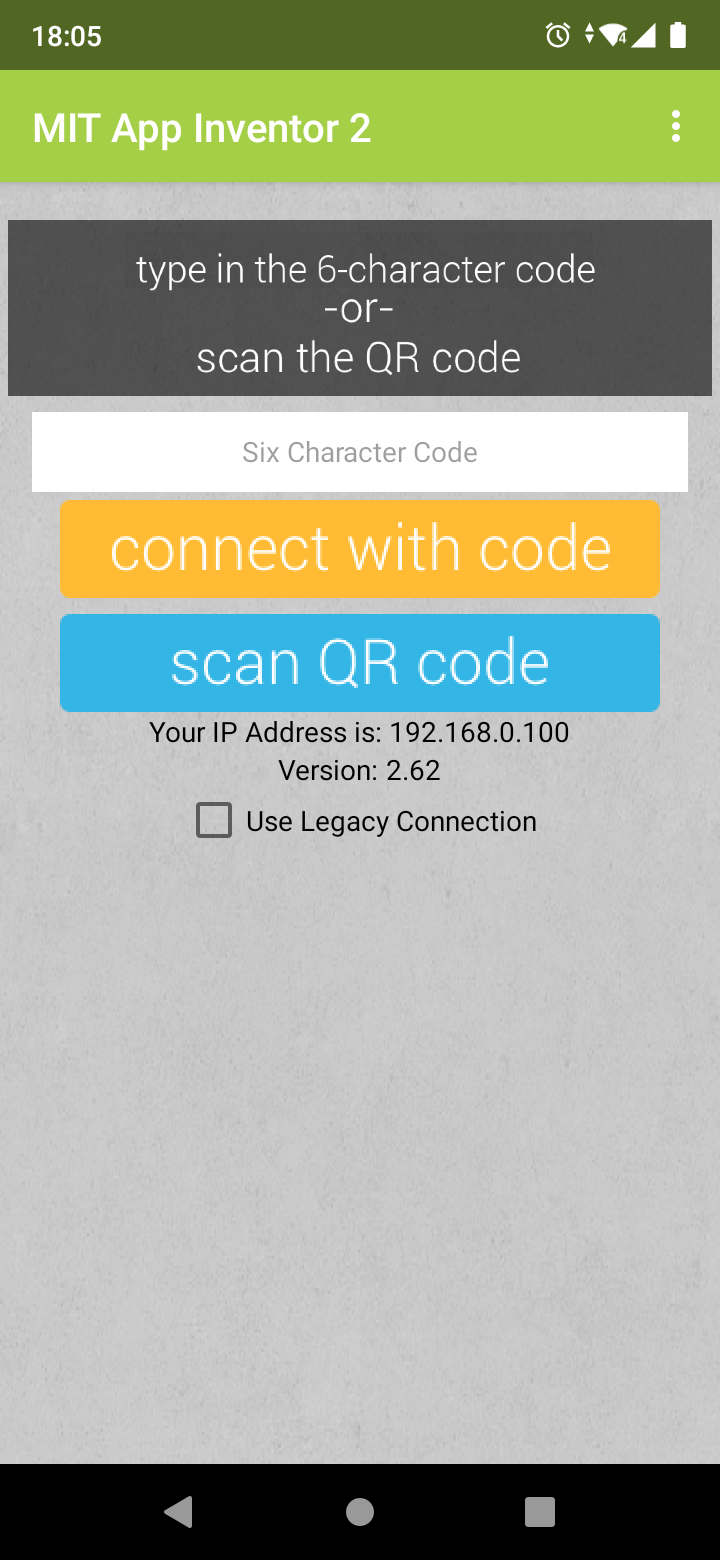
\includegraphics[width=\linewidth]{fig010042.png}
  \subcaption{\tiny Избор на инсталация}
  \label{fig010042}
  \end{subfigure}
  \begin{subfigure}{0.31\textwidth}
  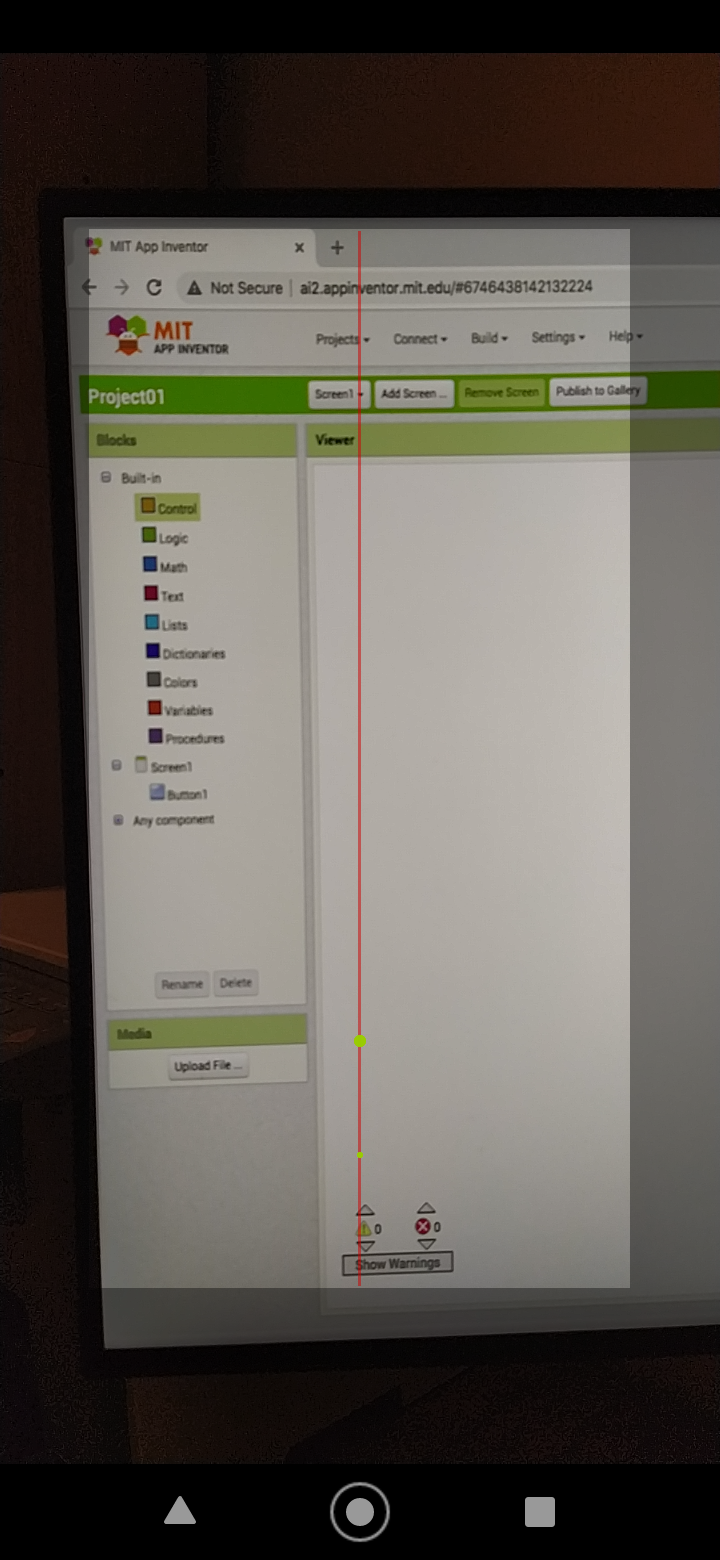
\includegraphics[width=\linewidth]{fig010043.png}
  \subcaption{\tiny Сканиране на код}
  \label{fig010043}
  \end{subfigure}
  \begin{subfigure}{0.31\textwidth}
  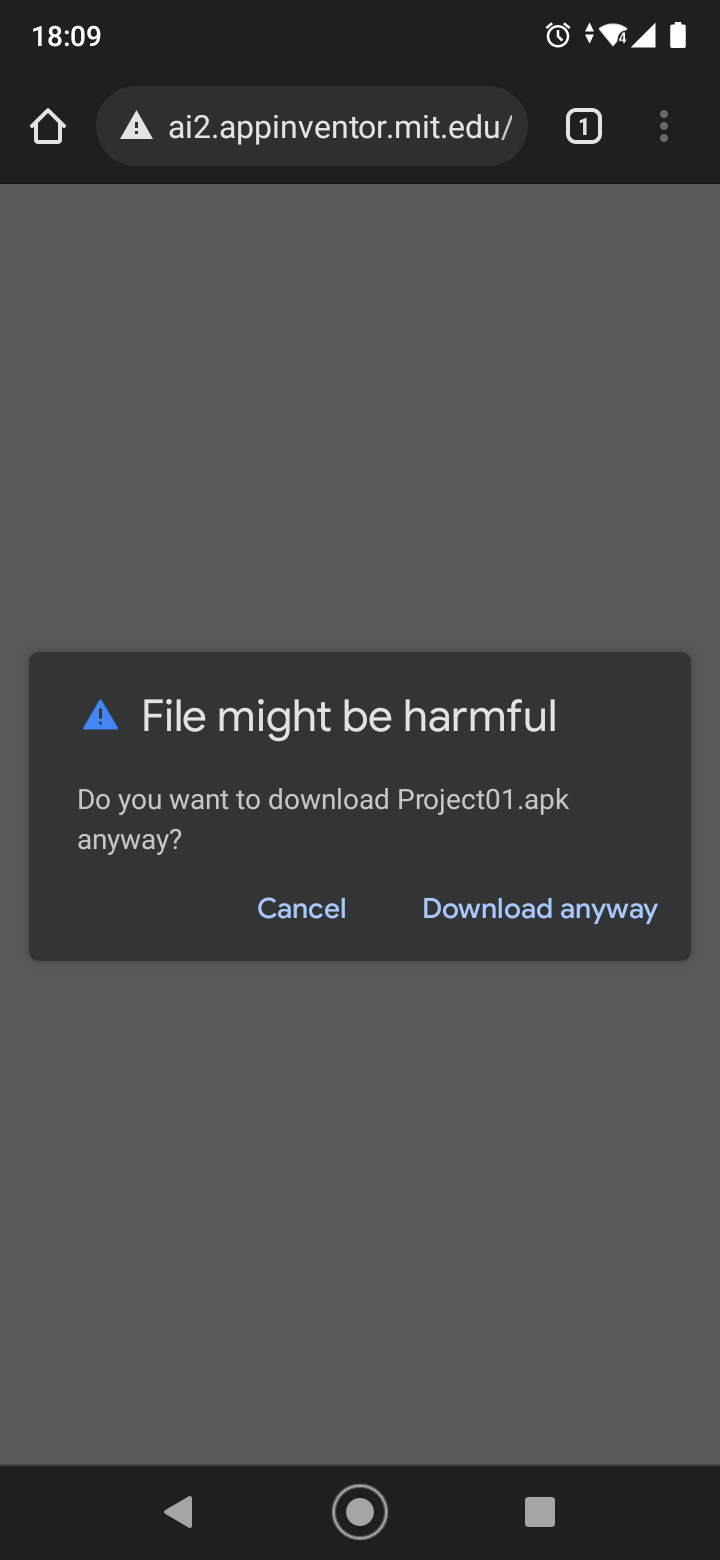
\includegraphics[width=\linewidth]{fig010044.png}
  \subcaption{\tiny Сваляне на файл}
  \label{fig010044}
  \end{subfigure}
  \caption{Инсталация през QR код}
\end{figure}

След като инсталационният пакет бива свален, операционната система издава съобщение за успешно извършена операция по запис на инсталатора (Фиг. \ref{fig010045}). Потребителят трябва да избере инсталационния пакет и да го активира. Това води до запитване дали действително желае да инсталира програмата, съдържана в сваления файл (Фиг. \ref{fig010046}). Въпреки, че ние сме наясно как точно е бил създаден инсталационният файл, операционната система го възприема, като програма създадена от непроверен разработчик. Поради тази причина, повторно задава въпрос на потребителя дали желае да направи инсталацията (Фиг. \ref{fig010047}). 

\begin{figure}[H]
  \begin{subfigure}{0.31\textwidth}
  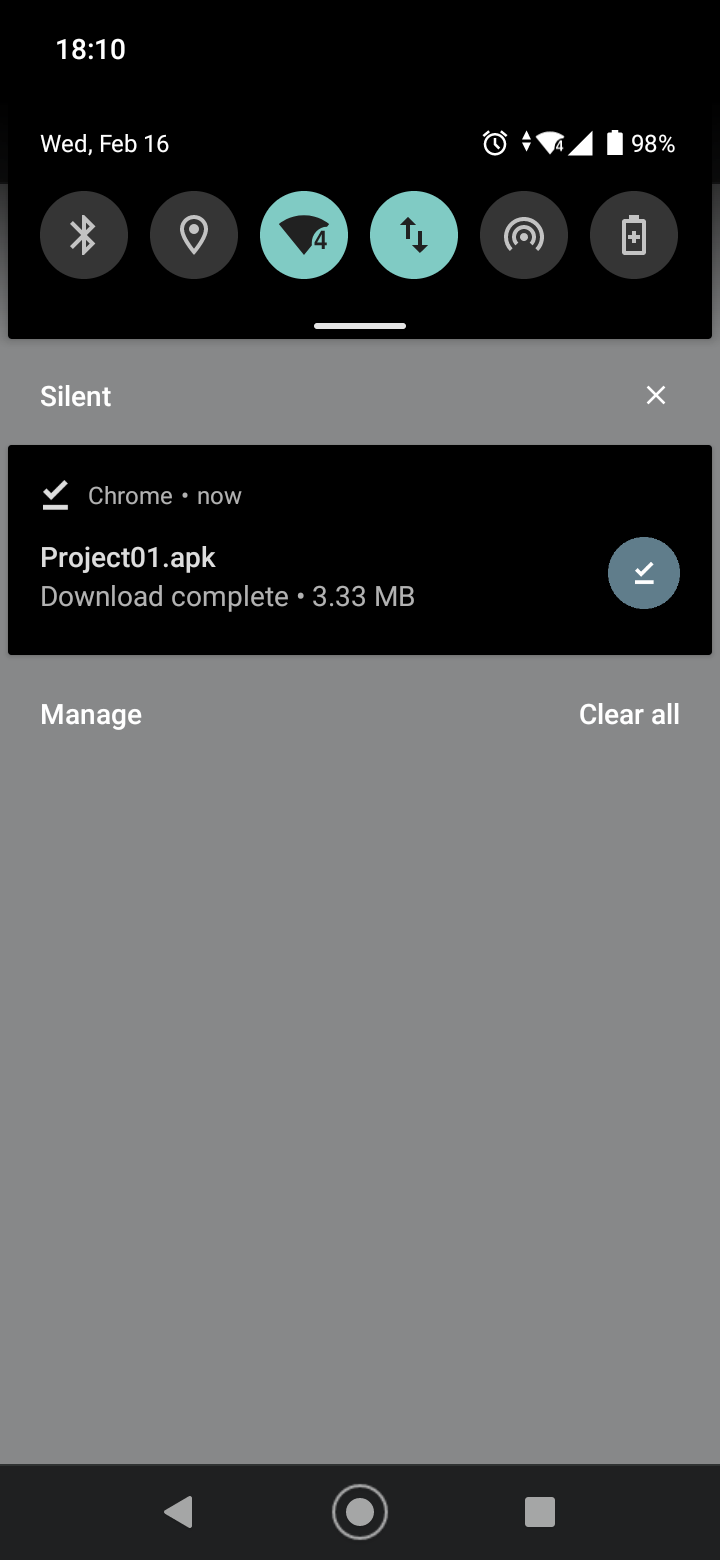
\includegraphics[width=\linewidth]{fig010045.png}
  \subcaption{\tiny Свален файл}
  \label{fig010045}
  \end{subfigure}
  \begin{subfigure}{0.31\textwidth}
  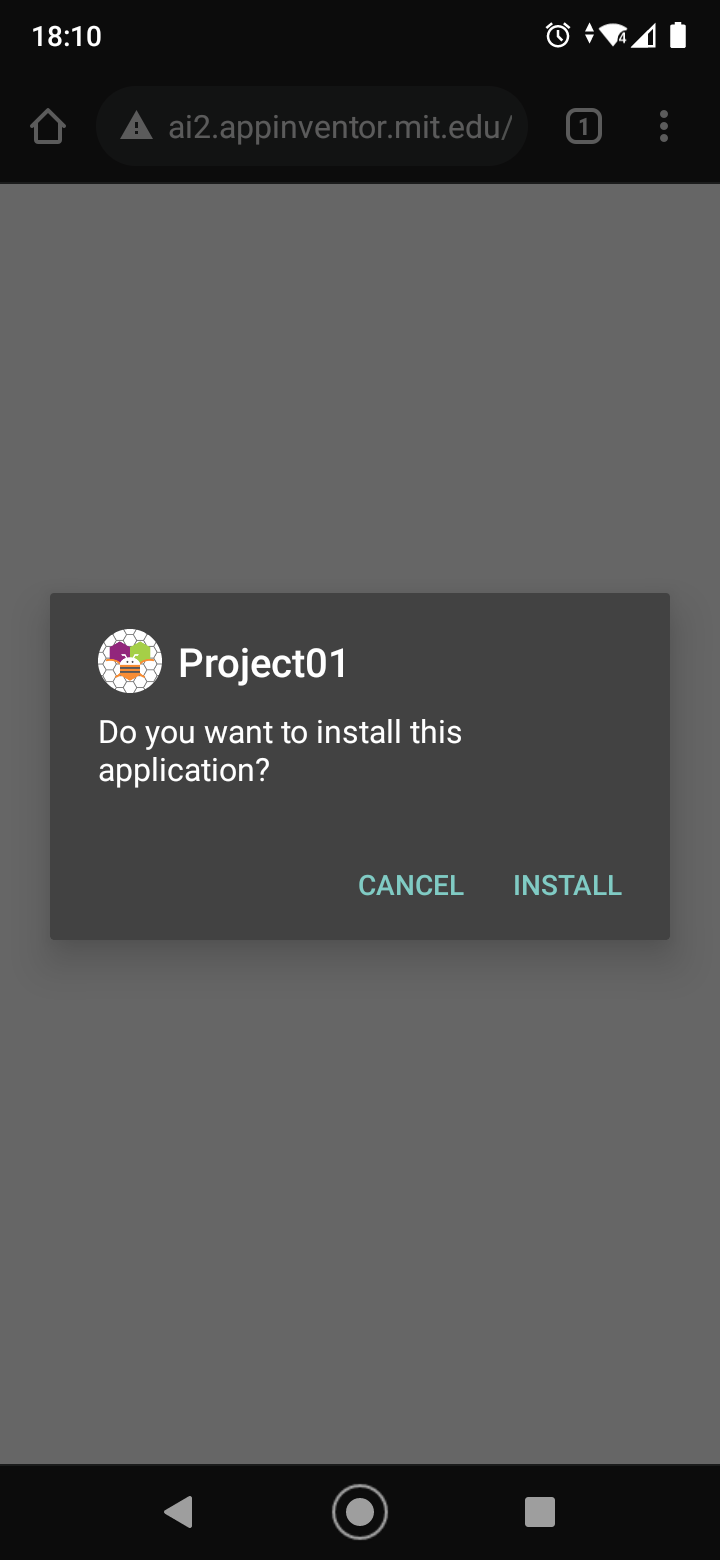
\includegraphics[width=\linewidth]{fig010046.png}
  \subcaption{\tiny Избор за инсталиране}
  \label{fig010046}
  \end{subfigure}
  \begin{subfigure}{0.31\textwidth}
  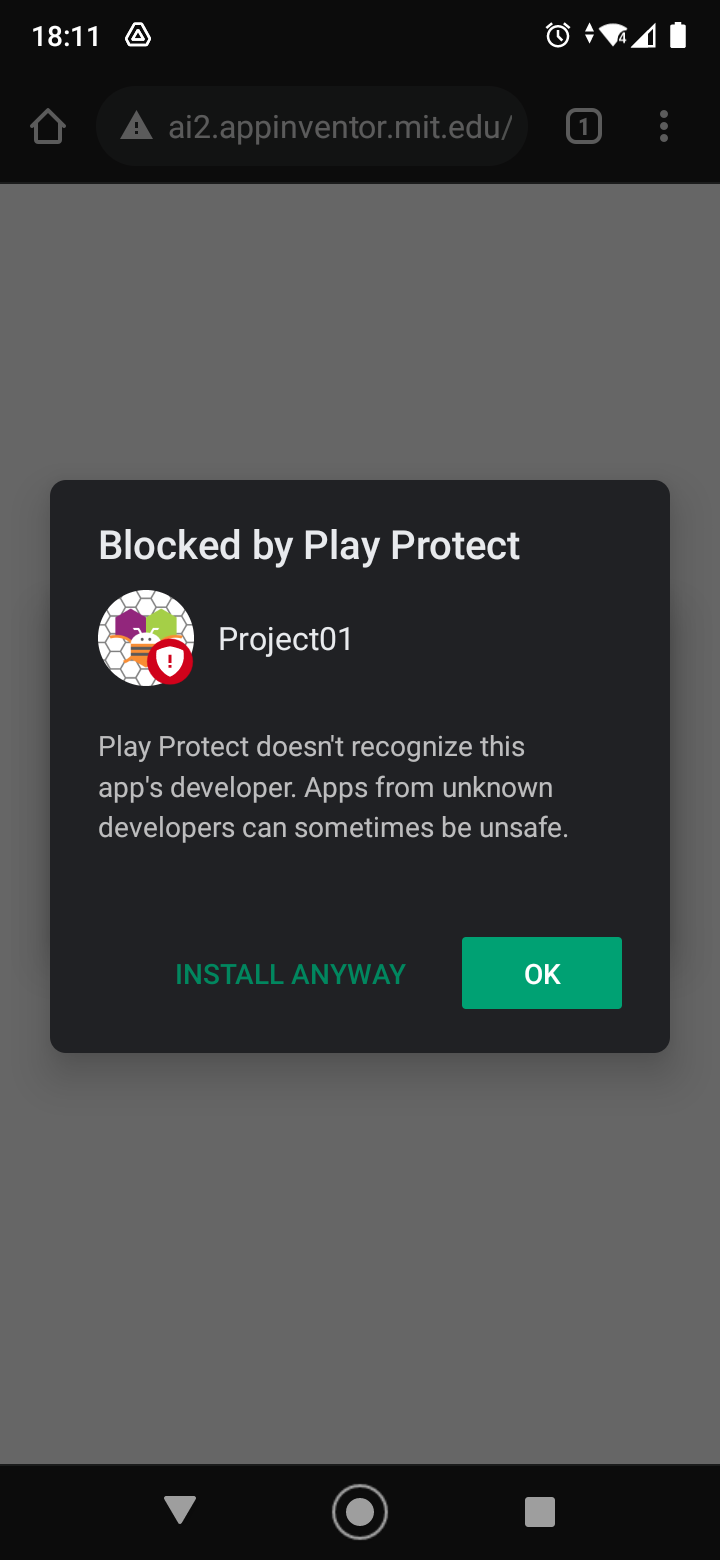
\includegraphics[width=\linewidth]{fig010047.png}
  \subcaption{\tiny Потвърждение за инсталиране}
  \label{fig010047}
  \end{subfigure}
  \caption{Инсталация върху мобилното устройство}
\end{figure}

Избира се „Install Anyway“ и написаната програма бива инсталирана върху мобилното устройство. Процесът по инсталацията завършва с подканящ прозорец за стартиране на новоинсталираната програма (Фиг. \ref{fig010048}). За да се провери работата на написания код е достатъчно да бъде натиснат визуализирания бутон в горния ляв ъгъл (Фиг. \ref{fig010049}). Резултатът от това действие е затваряне на прозореца и визуализиране на виртуалния тапет (Фиг. \ref{fig010049}).

\begin{figure}[H]
  \begin{subfigure}{0.31\textwidth}
  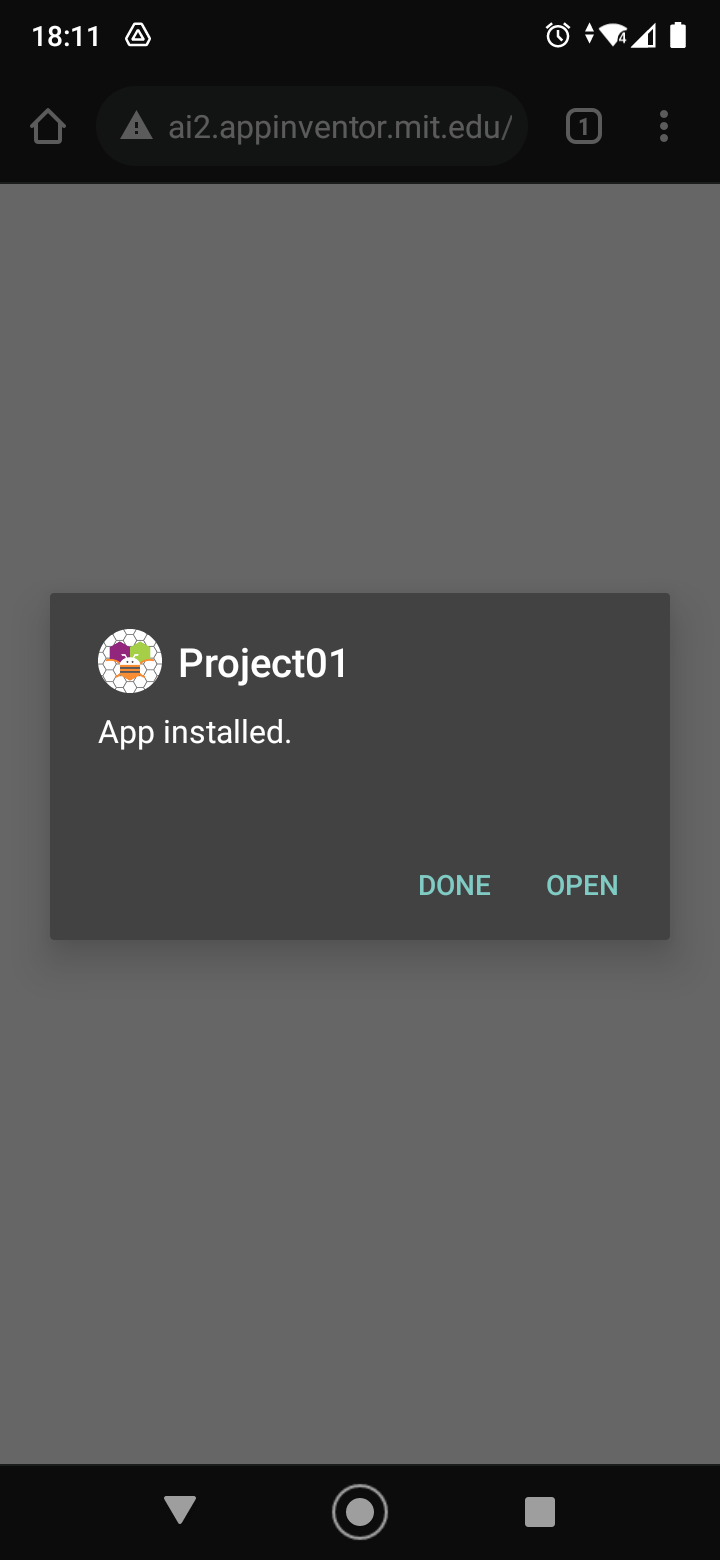
\includegraphics[width=\linewidth]{fig010048.png}
  \subcaption{\tiny Стартиране}
  \label{fig010048}
  \end{subfigure}
  \begin{subfigure}{0.31\textwidth}
  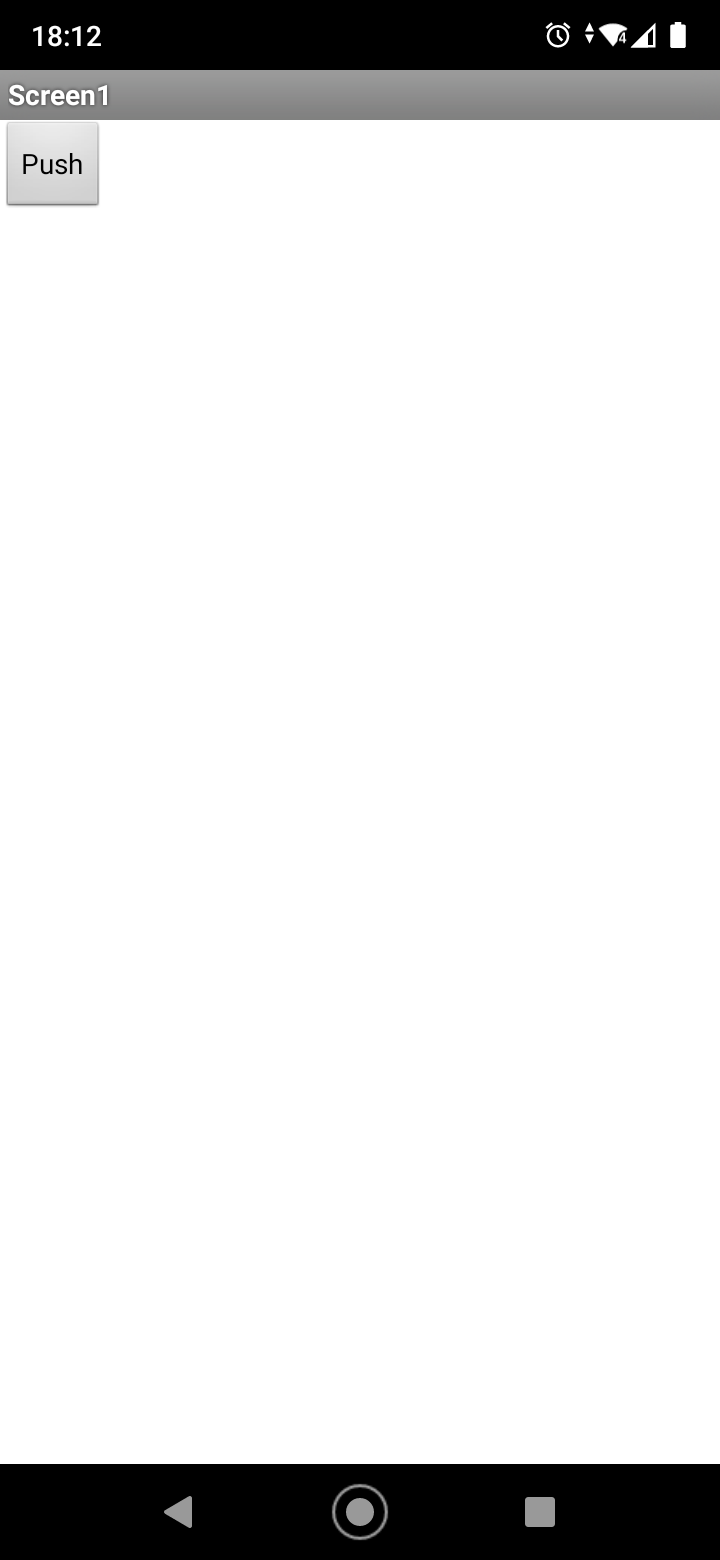
\includegraphics[width=\linewidth]{fig010049.png}
  \subcaption{\tiny Избор на бутона}
  \label{fig010049}
  \end{subfigure}
  \begin{subfigure}{0.31\textwidth}
  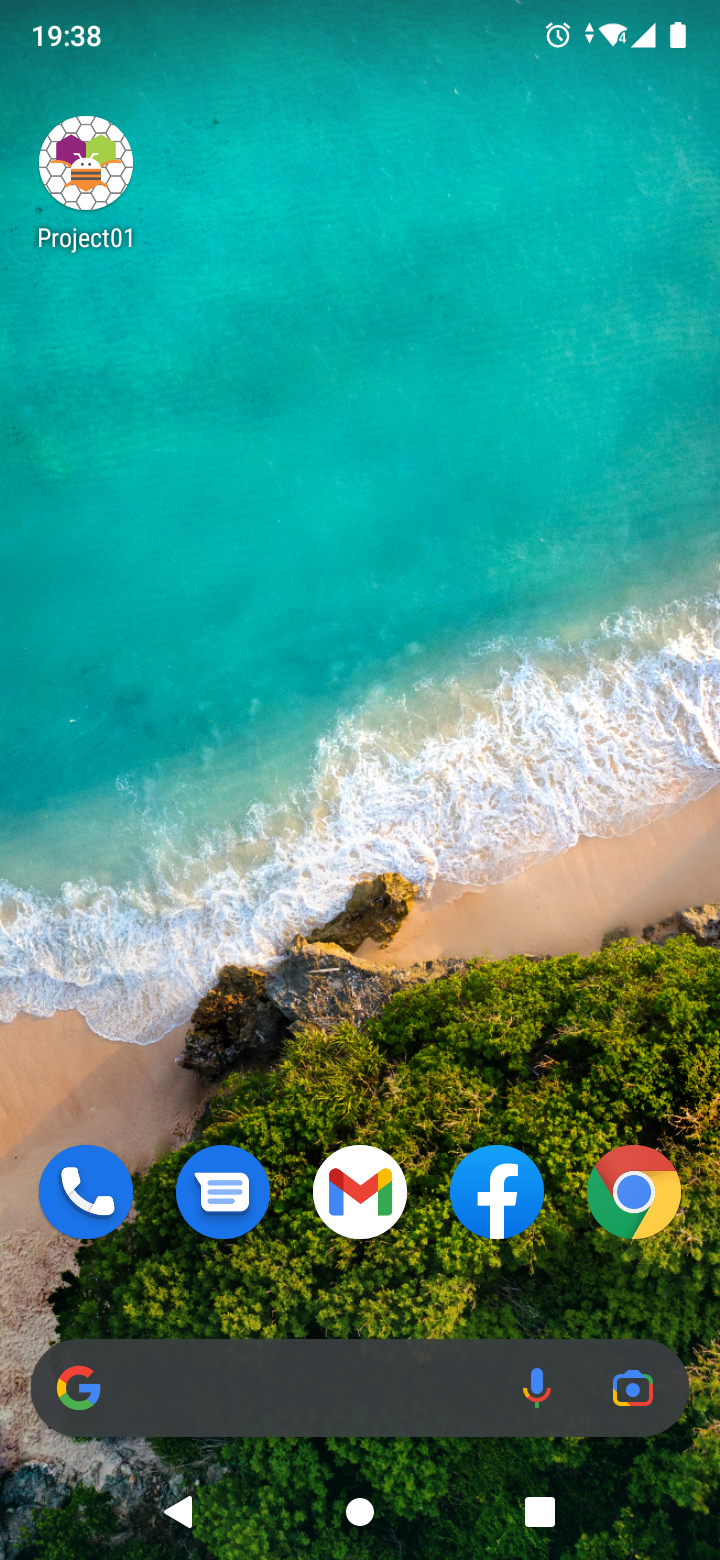
\includegraphics[width=\linewidth]{fig010050.png}
  \subcaption{\tiny Затворено приложение}
  \label{fig010050}
  \end{subfigure}
  \caption{Работа с приложението}
\end{figure}

При App Inventor най-очарователната част е, че разработените програми стават налични на мобилните устройства и човекът, който ги създава може да показва своята работа, дори когато не е пред компютър или не разполага с Интернет свързаност. 

